\documentclass{article}

\usepackage[czech]{babel}
\usepackage[T1]{fontenc}
\usepackage[utf8]{inputenc}

% Czech and German use the same quotes
\usepackage[style=german]{csquotes}

\usepackage[perpage]{footmisc} % per page numbering of footnotes
\usepackage{array}
\usepackage{multienum}

\usepackage{float}
\usepackage{graphicx}
\usepackage[dvipsnames]{xcolor}
\usepackage{booktabs} % toprule, midrule
\usepackage{longtable}
\usepackage{fancyvrb} % "Verbatim" (capital V) with font size

% References
\usepackage[unicode]{hyperref}
\hypersetup{
  colorlinks=true,
  linkcolor=black, % BrickRed
  urlcolor=blue,
  linkbordercolor=blue
}

% Math packages
\usepackage{amssymb}
\usepackage{amstext}
\usepackage{amsmath}
\usepackage{mathrsfs}
\usepackage{amsthm}
\usepackage{mathtools}
\usepackage{braket}
\usepackage{stmaryrd} % mapsfrom
\usepackage{physics} % \dv{s}{t} for derivative of s by t

\usepackage{algorithm} % this does the figure environment
\usepackage{algpseudocode} % algorithmicx, this does the actual algs

\usepackage{tikz}
\usepackage{tikz-cd}
\usetikzlibrary{automata,positioning}

\usepackage[capitalize,nameinlink,noabbrev]{cleveref} % has to be below amsthm

% Don't number algorithms
\makeatletter
\renewcommand{\fnum@algorithm}{\fname@algorithm}
\makeatother

% Fix the weird reference stuff
% https://tex.stackexchange.com/questions/177025/hyperref-cleveref-and-algpseudocode-same-identifier-warning
\makeatletter
\newcounter{algorithmicH}% New algorithmic-like hyperref counter
\let\oldalgorithmic\algorithmic
\renewcommand{\algorithmic}{%
  \stepcounter{algorithmicH}% Step counter
  \oldalgorithmic}% Do what was always done with algorithmic environment
\renewcommand{\theHALG@line}{ALG@line.\thealgorithmicH.\arabic{ALG@line}}
\makeatother

% Theorems, their numbering and style
\theoremstyle{plain}
\newtheorem{theorem}{Věta}[section]
\newtheorem{claim}[theorem]{Tvrzení}
\newcommand{\claimautorefname}{Tvrzení}
\newtheorem{lemma}[theorem]{Lemma}
\newtheorem{corollary}[theorem]{Důsledek}
\newtheorem{note}[theorem]{Poznámka}
\theoremstyle{definition}
\newtheorem{definition}[theorem]{Definice}
\newtheorem{example}[theorem]{Příklad}

%% Math operators

% Probability
\DeclareMathOperator{\Image}{Im}
\DeclareMathOperator{\Expect}{E}
\DeclareMathOperator{\Var}{Var}

\DeclareMathOperator{\true}{true}
\DeclareMathOperator{\false}{false}
\DeclareMathOperator{\mand}{\ \&\ } % to distinguish from \wedge
\DeclareMathOperator{\mor}{\ |\ } % to distinguish from \vee
\DeclareMathOperator{\lcm}{lcm}
\DeclareMathOperator{\barvee}{\overline{\vee}}
%\DeclareMathOperator{\barwedge}{\overline{\wedge}}
%\DeclareMathOperator{\eval}{eval}
\DeclareMathOperator{\id}{id}
\DeclareMathOperator{\Models}{Mod}
\DeclareMathOperator{\Id}{Id}

% Commands
\newcommand{\powerset}[1]{\mathcal{P}(#1)}
\newcommand{\finpowerset}[1]{\mathcal{P}^{\text{fin}}(#1)}
\newcommand{\downset}[1]{{\downarrow #1}}
\newcommand{\conggen}[1]{{\langle #1 \rangle_{\text{cong}}}}
\newcommand\logeq{\mathrel{\buildrel{def}\over\iff}}
\newcommand{\freealg}[2]{\mathcal{F}_{\mathcal{#1}}(#2)}
\DeclareMathOperator*{\argmin}{\arg\!\min}
\newcommand{\diff}[1]{\; \text{d} #1}
\newcommand{\Inf}[1]{\text{Inf}(#1)}

% Complexity classes, package `complexity` clashes with other packages
\newcommand{\ComplexityFont}[1]{{\ensuremath{\mathsf{#1}}}}
\renewcommand{\L}{\ComplexityFont{L}}
\renewcommand{\P}{\ComplexityFont{P}}
\newcommand{\NP}{\ComplexityFont{NP}}
\newcommand{\coNP}{\ComplexityFont{coNP}}
\newcommand{\PSPACE}{\ComplexityFont{PSPACE}}
\newcommand{\NPSPACE}{\ComplexityFont{NPSPACE}}
\newcommand{\ZPP}{\ComplexityFont{ZPP}}
\newcommand{\RP}{\ComplexityFont{RP}}
\newcommand{\coRP}{\ComplexityFont{coRP}}
\newcommand{\BPP}{\ComplexityFont{BPP}}
\newcommand{\FPTAS}{\ComplexityFont{FPTAS}}
\newcommand{\PTAS}{\ComplexityFont{PTAS}}
\newcommand{\APX}{\ComplexityFont{APX}}
\newcommand{\IP}{\ComplexityFont{IP}}
\newcommand{\CC}{\ComplexityFont{CC}}

% TikZ styles
\tikzset{%
    dot/.style={%
        draw, shape=circle, fill, inner sep=2pt
    }
}

\begin{document}

\title{Teoretická Informatika -- Státnicové Otázky}

\maketitle
\tableofcontents
\thispagestyle{empty} % do not show number
\clearpage % end page
\setcounter{page}{1} % reset counter to 1

\section{Pravděpodobnost}

\subsection{Úvod}
Dobrým zdrojom sú materiály z predmetu \verb|IV111| Probability in Computer Science.

Čo sa týka poslednej odrážky v otázke (\uv{aplikace v informace}), tu pôjde
zrejme najmä o~pravdepodobnostné algoritmy, ktoré popisujeme hlavne v~sekcii
{\uv{Algoritmy pro těžké problémy} (čiastočne aj v~sekciách \uv{Složitost} 
a \uv{Grafy a grafové algoritmy}).


\subsubsection*{Znenie otázky}
Pravděpodobnost. Základní pojmy a vlastnosti pravděpodobnosti; 
náhodná proměnná a její charakteristiky (střední hodnota, rozptyl, momenty, ....) 
a jejich použití; binomická, geometrická a další distribuce a jejich charakteristiky. 
Markovova a Čebyševova nerovnost a jejich použití; Černoffovy odhady a jejich použití; 
náhodné, zejména Markovovy, procesy a jejich vlastnosti; entropie a informace 
a jejich vlastnosti; aplikace v informatice.

\subsubsection*{Pojmy}
Náhodný pokus, základný priestor (konečný, spočetný, nespočetný); hod mincou, kockou;
jav (nemožný, istý, elementárny, opačný), de Morganove zákony, nezávislé 
javy (vzájomne, kolektívne), rozklad základného priestoru, 
pravdepodobnosť (diskrétna, spojitá), princíp inklúzie/exklúzie,
pravdepodobnostný priestor (diskrétny, spojitý), $\sigma$-field, 
podmienená pravdepodobnosť, zákon o totálnej pravdepodobnosti,
Bayesove pravidlá; náhodná premenná (diskrétna, spojitá), 
pravdivostná funkcia (distribúcia), distribučná funkcia, 
hustota, marginálna distribúcia, stredná hodnota, momenty,
rozptyl, smerodatná odchýlka, náhodná generujúca funkcia;
Bernoulliho rozdelenie, geometrické rozdelenie, binomické
rozdelenie, rovnomerné rozdelenie, exponenciálne rozdelenie,
normálne rozdelenie; Markovova nerovnosť, korelačný koeficient,
kovariancia, Chebyshevova nerovnosť; moment generujúce funkcie,
Chernoffove odhady; stochastické procesy (konečné, diskrétne,
spojité), Markovov reťazec, matica prechodu, iniciálny vektor,
hitting time, hitting probability, stavy Markovovho
modelu (absorbující, rekurentní, průchozí), ireducibilný Markov Chain (MC),
stacionárna distribúcia, periodický/aperiodický MC;
entropia (Shannon), joint entropy, podmienená entropia, 
entropy chain rule, relatívna entropia, spoločná informácia.

\subsection{Základní pojmy a vlastnosti pravděpodobnosti}

\begin{definition}
Pro daný náhodný experiment je diskrétní pravděpodobnostní prostor trojice
$(\Omega, \mathcal{F}, P)$,
kde
\begin{itemize}
    \item $\Omega$ je množina možných výsledků experimentu,
    \item $\mathcal{F} \subseteq \powerset{\Omega}$ je množina možných události (javov),
    \item $P : \mathcal{F} \to [0,1]$ je pravděpodobnostní funkce, tedy
        pro po párech disjunktní $\{A_i\}_{i=1}^\infty \subseteq \mathcal{F}$ platí
        $P(\bigcup A_i) = \sum P(A_i)$ a $P(\Omega) = 1$.
\end{itemize}
\end{definition}

\begin{example}
    Můžeme například uvažovat experiment hodu dvěma kostkami.
    $\Omega = \{1,\ldots,6\}^2$, pro diskrétní $\Omega$ platí
    $\mathcal{F} = \powerset{\Omega}$ a z~uniformity kostek
    $P((x,y)) = 1/\lvert \Omega \rvert, (x,y) \in \Omega$.
\end{example}

Špeciálne prípady pri javoch sú istý jav (celá množina $\Omega$, určite nastane),
nemožný jav (prázdna množina $\emptyset$, nikdy nenastane),
elementárny jav (napr. to, že pri hode kockou padne práve 1,
neelementárnym javom by bol napr. jav, že padne nepárne číslo,
ktorý je zložený z troch elementárnych javov).

\begin{definition}
	Javy $A_1, \ldots, A_n$ nazývame {\em vzájomne disjunktné}, 
	pokiaľ platí $\forall i \neq j.P(A_i \land A_j)=0$.
	
	Javy $A_1, \ldots, A_n$ nazývame {\em kolektívne vyčerpávajúce}, %spravny termin? 
	pokiaľ platí $P(A_1 \lor \ldots \lor A_j)=1$.
	
	Javy $A_1, \ldots, A_n$ sú {\em rozkladom} základného priestoru,
	pokiaľ sú vzájomne disjunktné a kolektívne vyčerpávajúce.
\end{definition}

\begin{claim}
    Nechť $A$ je událost a $\overline{A}$ její doplněk. Pak
    $P(\overline{A}) = 1 - P(A)$.
\end{claim}

\begin{proof}
    Víme $P(A \cup \overline{A}) = 1$ a $P(A \cap \overline{A}) = 0$,
	tedy $P(A) + P(\overline{A}) - P(A \cap \overline{A}) = P(A) + P(\overline{A}) = 1$.
\end{proof}

\begin{definition}
Podmíněnou pravděpodobnost výskytu události $A$ za předpokladu výskytu
události $B$ definujeme
\[
    P(A \mid B) = \frac{P(A \cap B)}{P(B)}
\]
\end{definition}

Jednoduchou intuici za definicí nabízí Vennův diagram.

\begin{theorem}[Totální pravděpodobnosti]
	Nech javy $B_i$ sú rozkladom základného priestoru. Potom
    \[
        P(A) = \sum_i P(A \cap B_i) = \sum_i P(A \mid B_i) P(B_i)
    \]
\end{theorem}

\begin{example}
    Žárovky X svítí přes 5000 hodin v~99 \% případů.
    Žárovky Y svítí přes 5000 hodin v~95 \% případů.
    Žárovky X tvoří 60 \% dostupných žárovek.
    Žárovky Y tvoří 40 \% dostupných žárovek.
    Jaká je pravděpodobnost, že náhodně zvolená žárovka
    bude svítit přes 5000 hodin?
    \[
{\displaystyle {\begin{aligned}\Pr(A)&=\Pr(A\mid B_{X})\cdot \Pr(B_{X})+\Pr(A\mid B_{Y})\cdot \Pr(B_{Y})\\[4pt]&={99 \over 100}\cdot {6 \over 10}+{95 \over 100}\cdot {4 \over 10}={{594+380} \over 1000}={974 \over 1000}\end{aligned}}}
\]
\end{example}

\begin{theorem}[Bayes]
    Pokud $P(B) \neq 0$, pak
    \[
    P(A \mid B) = \frac{P(B \mid A)P(A)}{P(B)}
    \]
\end{theorem}

Věta vyplývá z~jednoduché úpravy definice podmíněné pravděpodobnosti.

\begin{example}
    % https://www.wikiskripta.eu/w/Bayesova_v%C4%9Bta
Předpokládejme, že máme školu s~60~\% chlapců
a 40~\% dívek. Všichni chlapci nosí kalhoty.
Z~dívek nosí kalhoty polovina. Pozorovatel vidí z~dálky studenta v kalhotách.
Jaká je pravděpodobnost, že tento student je dívka?
Jako událost G označíme, že pozorovaný student je dívka. Jako událost T,
že pozorovaný student nosí kalhoty. Chceme vypočíst $P(G \mid T)$.
\[
    P(G \mid T)
    = \frac{P(T \mid G)P(G)}{P(T)}
    = \frac{1/2 \cdot 4/10}{6/10 \cdot 1 + 4/10 \cdot 1/2}
	= \frac{1}{4}
\]
\end{example}

Keď je základný priestor $S$ spojitý, dá sa miesto neho
v určitých prípadoch použiť $\sigma$-field.

\begin{definition}
	Nech $S$ je spojitý základný priestor. Potom $\mathscr{F} \subseteq 2^S$
	je $\sigma$-field, pokiaľ
	\begin{itemize}
		\item $\emptyset \in \mathscr{F}$
		\item $A,B \in \mathscr{F} \Rightarrow A \cup B \in \mathscr{F}$
		\item $A \in \mathscr{F} \Rightarrow \overline{A} \in \mathscr{F}$
	\end{itemize}
\end{definition}

Poznamenajme, že vďaka De Morganovym zákonom je $\sigma$-field uzavretý
aj na prienik.

\subsection{Náhodná proměnná a její charakteristiky}

\begin{definition}
    Pro (diskrétní) pravděpodobnostní prostor $(\Omega, \mathcal{F}, P)$
    nazveme {\em (diskrétní) náhodnou proměnnou} funkci $X : \Omega \to \mathbb{R}$.
\end{definition}

\begin{example}
    Například pro
    $(\{1,\ldots,6\}, \powerset{\{1,\ldots,6\}}, P(x) = 1/6)$
    můžeme definovat náhodnou proměnnou
    $X(x) = 0, x = 1,\ldots,5, X(6) = 1$.
\end{example}

\begin{definition}
    Pravdepodobnostná funkcia (alebo pravdepodobnostná distribúcia)
	náhodnej premennej $X$ je funkcia $p_X: \mathbb{R} \to [0,1]$ definovaná ako
	\[
    p_X(x) = P(X=x) = \sum_{s:X(s)=x}P(s)
    \]
\end{definition}

\begin{definition}
    Distribučná funkcia
	náhodnej premennej $X$ je funkcia $F_X: \mathbb{R} \to [0,1]$ definovaná ako
	\[
    F_X(x) = P(X\leq x) = \sum_{t \leq x}p_X(t)
    \]
\end{definition}

Pre distribučnú funkciu platí:
\begin{enumerate}
	\item pre $-\infty < x < \infty$ platí $0 \leq F(x) \leq 1$
	\item F(x) je neklesajúca funkcia
	\item $lim_{x \to -\infty}F(x) = 0$ a $lim_{x \to \infty}F(x) = 1$
	\item TODO
\end{enumerate}

V prípade spojitej distribúcie nemá zmysel hovoriť o pravdepodobnostnej
funkcii. V tomto prípade sa používa {\em hustota}, ktorá je definovaná
ako derivácia distribučnej funkcie.

\begin{definition}[Očekávaná (střední) hodnota]
    Nechť $(\Omega, \mathcal{F}, P)$ je diskrétní pravděpodobnostní
    prostor a $X$ náhodná proměnná. {\em Očekávaná hodnota} $X$
    je
    \[ \Expect(X) = \sum_{x \in \Image(X)} x \cdot P(X = x) \]
\end{definition}

\begin{theorem}
    Nechť $(X_i)_{i=1}^{n}$, $n \in \mathbb{N}$, je posloupnost
    náhodných proměnných \linebreak s~konečnou očekávanou hodnotou, potom
    \[
        E \big ( \sum X_i \big ) = \sum E(X_i)
    \]
\end{theorem}

\begin{proof}
    Indukcí k~počtu sčítanců. Bázový případ je triviální. Nechť $X$ je
    náhodná proměnná a $Y$ je součtem nenulového počtu náhodných proměnných.

    \begin{align*}
        E(X + Y) &= \sum_i \sum_j (i+j) P((X = i) \cap (Y = j)) \\
                 &= \sum_i \sum_j i P((X = i) \cap (Y = j))
                  + \sum_i \sum_j j P((X = i) \cap (Y = j)) \\
                 &= \sum_i i \sum_j P((X = i) \cap (Y = j))
                  + \sum_j j \sum_i P((X = i) \cap (Y = j)) \\
                 &= \sum_i i P(X = i)
                  + \sum_j j P(Y = j) \\
                 &= E(X) + E(Y)
                   \qedhere
    \end{align*}
\end{proof}

\begin{theorem}
    \[
        E(cX) = cE(X)
    \]
\end{theorem}

\begin{proof}
    Pro $c = 0$ je tvrzení zřejmé. Pro $c \neq 0$ platí

    \begin{align*}
        E(cX) &=   \sum_i i P(cX = i) \\
              &= c \sum_i (i/c) P(X = i/c) \\
              &= c \sum_j j P(X = j) \\
              &= c E(X)
                \qedhere
    \end{align*}
\end{proof}

\begin{definition}
    Proměnné $X,Y$ nazveme {\em nezávislé} pokud pro všechna $x,y$
    \[
        P(X = x \land Y = y) = P(X = y) P(Y = y)
    \]
\end{definition}

Alternativně $P(X = x \mid Y = y) = P(X = x)$ pro každé $x,y$. (Tady by
bylo dobré si rozmyslet, proč tomu tak je.)

\begin{definition}[Momenty]
    Pre náhodnú premennú $X$ je $k$-ty {\em moment}
	definovaný ako $\Expect(X^k)$ a $k$-ty {\em centrálny moment}
	ako $\Expect((X-\Expect(X))^k)$.
\end{definition}

\begin{definition}[Rozptyl, variance]
    Pro náhodnou proměnnou $X$ je {\em rozptyl}
    \[ \Var(X) = \Expect( (X - \Expect(X))^2 ) \]
\end{definition}

Na rozptyl se tedy můžeme dívat jako na druhou mocninu očekávané
vzdálenosti od očekávané hodnoty. Druhá odmocnina rozptylu je
{\em standardní odchylka}.

Všimnime si, že rozptyl je druhým centrálnym momentom.

Následující tvrzení se snadným důkazem dává užitečný způsob výpočtu
variance.

\begin{claim}
    $ Var(X) = \Expect( (X - \Expect(X))^2 ) = \Expect(X^2) - \Expect(X)^2 $
\end{claim}

\begin{definition}[Kovariance]
    $ Cov(X,Y) = E((X - E(X))(Y - E(Y))) $
\end{definition}

Na kovarianci se můžeme dívat jako na míru společné variance dvou
proměnných.

\begin{claim}
    $Var(X + Y) = Var(X) + Var(Y) + 2 Cov(X,Y)$
\end{claim}

\begin{theorem}
    Jsou-li $X, Y$ nezávislé náhodné proměnné, potom
    \[ E(X \cdot Y) = E(X) \cdot E(Y) \]
\end{theorem}


\begin{corollary}
    Jsou-li $X, Y$ nezávislé náhodné proměnné, pak $Cov(X,Y) = 0$.
\end{corollary}

\begin{proof}
    Jsou-li $X, Y$ nezávislé, potom i $X - E(X)$ a $Y - E(Y)$ jsou
    nezávislé. Můžeme tedy použít větu o násobení nezávislých
    očekávaných hodnot. Potom $E(Z - E(Z)) = E(Z) - E(E(Z)) = 0$.
\end{proof}

\subsection{Distribuce}

\begin{definition}[Uniformní rozdělení]
    Náhodná proměnná $X$ má {\em uniformní distribuci},
    pokud pro všech $K$ hodnot $k$ platí
    \[
        P(X = k) = 1/K
    \]
\end{definition}

\begin{definition}[Bernoulliho rozdělení]
    Náhodná proměnná $X$ má {\em Bernoulliho distribuci} s~parametrem
    $p$, pokud
    \begin{align*}
        P(X = 1) &= p  \\
        P(X = 0) &= 1 - p
    \end{align*}
\end{definition}

Z~definice vyplývá $E(X) = 1 \cdot p + 0 \cdot (1-p) = p$.

\begin{example}
    Príkladom náhodnej premennej s Bernoulliho distribúciou
	je hod nevyváženou mincou, kde hlava padne s pravdepodobnosťou $p$.
\end{example}

\begin{definition}[Binomické rozdělení]
    Náhodná proměnná $X$ má {\em binomickou distribuci} s parametry $(n, p)$,
    pokud pro $0 \leq k \leq n$ platí
\[
    P(X = k) = {{n} \choose {k}} p^k (1 - p)^{n - k}
\]
\end{definition}

\begin{theorem}
    \[
        X \sim Bin(n,p) \implies E(X) = np
    \]
\end{theorem}

\begin{proof}
    Uvažujme $n$ náhodných proměnných $X_i$ s~Bernoulliho distribucí
    s~parametrem $p$.
    Zřejmě $X \sim \sum X_i$, potom
    \[
        E(X) = E( \sum_{i = 1}^{n} X )
             = \sum_{i = 1}^{n} E(X)
             = \sum_{i = 1}^{n} p
             = n p
    \]
\end{proof}

\begin{example}
    Příkladem náhodné proměnné s~binomickým rozdělením je
    počet hlav, které padnou při $n$ hodech mincí ($p = 1/2$).
    Podle věty získáme očekávanou hodnotu $n/2$.
\end{example}

\begin{definition}[Geometrické rozdělení]
    Náhodná proměnná $X$ má {\em geometrickou distribuci} s~parametrem
    $p$, pokud pro $1 \leq k$ platí
\[
    P(X = k) = (1-p)^{k-1} p
\]
\end{definition}

\begin{claim}
    Geometrické rozdělení nemá paměť, tedy
    \[
        P(X = n + k \mid X > k) = P(X = n)
    \]
\end{claim}

\begin{theorem}
    Nechť $X$ je náhodná proměnná s~náhodným rozdělením s~parametrem
    $p$, potom
    \[
        E(X) = \frac{1}{p}
    \]
\end{theorem}

\begin{example}
    Novomanželé si plánují pořizovat děti, dokud se jim nenarodí dcera.
    Pravděpodobnost, že se jim narodí jediné dítě (a tedy dcera) je $1/2$.
    Pravděpodobnost, že se jim narodí dvě děti je $1/4$.
    Pravděpodobnost, že se jim narodí tři děti je $1/8$.
    Očekávaný počet dětí je $2$, tedy jeden syn a jedna dcera.

    Tento příklad také demonstruje, že geometrické rozdělení nemá paměť.
    Je jedno kolik dětí se dosud narodilo, pravděpodobnost narození
    dalších to nijak neovlivňuje.
\end{example}

\begin{definition}[Spojité uniformné rozdelenie]
    Spojitá náhodná premenná $X$ má {\em uniformnú distribúciu},
    pokiaľ pre jej hustotu platí
    \[
        f(x) = 
			\begin{cases}
				\frac{1}{b-a} &\quad x \text{ leží v intervale }[a,b]\\
				0 &\quad\text{inak}
			\end{cases}
    \]
\end{definition}

Pre distribučnú funkciu spojitej uniformnej náhodnej premennej teda platí
	\[
        F(x) = 
			\begin{cases}
				0 &\quad x < a \\
				\frac{x-a}{b-a} &\quad x \text{ leží v intervale }[a,b)\\
				1 &\quad x \geq b
			\end{cases}
    \]

\begin{definition}[Exponenciálne rozdelenie]
    Spojitá náhodná premenná $X$ má {\em exponenciálnu distribúciu}
    s parametrom $\lambda$, pokiaľ pre jej hustotu platí
    \[
        f(x) = \lambda e^{-\lambda x}
    \]
\end{definition}

Pre distribučnú funkciu exponenciálnej náhodnej premennej platí
	\[
        F(x) = 1-e^{-\lambda x}
    \]

\begin{definition}[Normálne rozdelenie]
    Spojitá náhodná premenná $X$ má {\em normálnu distribúciu}
    s parametrami $\mu$ (priemer) a $\sigma$ (rozptyl), pokiaľ pre jej hustotu platí
    \[
        f(x) = \frac{1}{\sqrt{2 \pi \sigma^2}}e^{-\frac{(x-\mu)^2}{2\sigma^2}}
    \]
\end{definition}

Pre distribučnú funkciu normálnej náhodnej premennej platí
	\[
        F(x) = \frac{1}{2} \left( 1+ \text{erf}\left(\frac{x-\mu}{\sigma \sqrt{2}}\right) \right),
    \]
kde erf značí error function.

\subsection{Markovova a Čebyševova nerovnost}

\begin{theorem}[Markovova nerovnost]
    Nechť $X$ je náhodná proměnná, která nabývá pouze nezáporných
    hodnot. Potom pro všechna $a > 0$,
    \[
       P(X \geq a) \leq \frac{E(X)}{a}
\]
\end{theorem}

\begin{proof}
    Pro $a \geq 0$ mějme
    \[
        I =
        \begin{cases}
            1, \quad \text{pokud } X \geq a, \\
            0, \quad \text{jinak.}
        \end{cases}
    \]
    Protože $I$ má Bernoulliho rozdělení, tak platí $E(I) = P(I = 1) = P(X \geq a)$.
    Navíc protože $X \geq 0$, tak platí $I \leq \frac{X}{a}$, na což
    aplikujeme $E$ a získáme
    \[
        P(X \geq a) = E(I) \leq E \left(\frac{X}{a} \right) = \frac{E(X)}{a}
        \qedhere
    \]
\end{proof}

\begin{example}
    Předpokládejme $n$-krát opakovaný experiment hodu mincí,
    a $X_i = 1$ padla-li hlava, $X_i = 0$ jinak.
    Potom $X = \sum X_i$ značí počet padlých hlav. Nyní můžeme snadno
    spočítat horní odhad na pravděpodobnost, že padne více než $3n/4$
    hlav.

    \[
        P(X \geq 3n/4) \leq \frac{n/2}{3n/4} = \frac{2}{3}
    \]
\end{example}

\begin{theorem}
    Pokud známe pouze $E(X)$ a fakt, že $X$ nenabývá záporných hodnot,
    potom Markovova nerovnost je těsná.
\end{theorem}

\begin{proof}
    Nechť $X = k$ s pravděpodobností $1$
    a $X = 0$ s~pravděpodobností $0$.
    Potom $P(X \geq k) = \frac{E(X)}{k}$.
\end{proof}

Pro aplikaci Markovovy nerovnosti stačila znalost prvního momentu
($\Expect(X)$). Se znalostí druhého momentu ($\Expect(X^2)$) můžeme
odvodit podstatně silnější nerovnost.

\begin{theorem}[Čebyševova nerovnost]
    Pokud $a \geq 0$, pak
    \[
        P(\lvert X - \Expect(X) \rvert \geq a) \leq \frac{\Var(X)}{a^2}
    \]
\end{theorem}

\begin{proof}
    Nejprve pozoroujeme, že
    \[
        P(\lvert X - \Expect(X) \rvert \geq a)
        = P((X - E(X))^2 \geq a^2)
\]
    potom pouze použijeme Markovovu nerovnost
    \[
        P((X - \Expect(X))^2 \geq a^2)
        \leq \frac{\Expect((X - \Expect(X))^2)}{a^2}
        = \frac{\Var(X)}{a^2}
        \qedhere
    \]
\end{proof}

\begin{example}
    Analyzujeme znovu příklad s~pravděpodobností, že padne více než
    $3n/4$ hlav z~$n$ hodů mincí. Nejprve ověříme, že
    \[
        \Expect((X_i)^2) = \Expect(X_i) = 1/2
    \]\[
        Var(X_i) = \Expect((X_i)^2) - \Expect(X_i)^2 = 1/4
    \]
    Nyní s~použítím linearity sčítání nekovariantních náhodných
    proměnných
    \[
        \Var(X) = \Var(\sum X_i) = \sum \Var(X_i) = n/4
    \]
    Aplikujeme Čebyševovu nerovnost
    \[
        P(X \geq 3n/4 ) \leq P(\lvert X - \Expect(X) \rvert \geq n/4)
                     \leq \frac{\Var(X)}{(n/4)^2}
                     = \frac{n/4}{(n/4)^2}
                    = \frac{4}{n}
    \]

    Protože nerovnost omezuje pravděpodobnost ze dvou stran (ze symetrie
    dané absolutní hodnotou), získáváme ještě přesnější odhad $2/n$.
\end{example}

\subsection{Chernoffovy odhady}

% http://math.mit.edu/~goemans/18310S15/chernoff-notes.pdf

Se znalostí všech momentů náhodné proměnné můžeme odvodit ještě silnější
odhady pravděpodobností.

\begin{definition}
    Funkci $M_X(s) = \Expect(e^{s X})$ nazveme {\em generátor momentů}.
\end{definition}

Důvodem pro název je Taylorův rozvoj
$M_X(s)
= \Expect( 1 + sX + \frac{1}{2!}s^2 X^2 + \frac{1}{3!}s^3 X^3 + \ldots )
= \sum_{i = 0}^{\infty} \frac{1}{i!} s^i \Expect (X^i)$
a z něj vyplývající tvrzení (za předpokladu, že $\Expect$ a derivace
pro dané $X$ komutují) $\Expect(X^n) = M^{(n)}_X(0)$, kde $(n)$ značí $n$-tou
derivaci.

\begin{theorem}
    Pokud $X, Y$ jsou nezávislé, pak
    \[
        M_{X+Y}(t) = M_X(t) M_Y(t)
    \]
\end{theorem}

Důkaz je snadný z~definice.

Obecně Chernoffovy odhady jsou získány aplikací Markovovy nerovnosti na
$e^{tX}$ pro vhodně zvolené $t$. Z Markovovy nerovnosti pro každé $t >
0$ platí
\[
    P(X \geq a) = P(e^{tX} \geq e^{ta}) \leq \frac{\Expect(e^{tX})}{e^{ta}}
\]
zejména tedy
\[
    P(X \geq a) \leq \min_{t > 0} \frac{\Expect(e^{tX})}{e^{ta}}
\]
Stejně tak platí opačná nerovnost pro $t < 0$.

%Odvodíme Chernoffův odhad pro součet Poissonových pokusů\footnote{To je téměř
%jako součet Bernoulliho pokusů, jen každý Poissonův pokus může mít jinou
%pravděpodobnost, zatímco od Bernoulliho očekáváme stejnou ve všech
%případech.}.

Jeden z~Chernoffových odhadů je následující.

\begin{theorem}
    Nechť $X = \sum X_i$, kde $X_i$ je Poissonovo s~$p_i$,
    všechny $X_i$ jsou nezávislé a nechť $\delta \in (0,1)$.
    \[
        P(X \geq (1 + \delta) \Expect(X)) \geq e^{- \Expect(X) \delta^2 / 3}
    \]
\end{theorem}

\begin{proof}[Náčrt důkazu]
% Slidy IV111
% Probability and Computing (Mitzenmacher, Upfal)
% https://www.cs.cmu.edu/afs/cs/academic/class/15859-f04/www/scribes/lec9.pdf
% http://math.mit.edu/~goemans/18310S15/chernoff-notes.pdf

Začneme výpočtem $M_X(t) = \Expect(e^{tX})$, na což
ovšem potřebujeme $M_{X_i}(t)$.
\begin{align*}
    M_{X_i}(t) &= \Expect(e^{t X_i}) \\
    &= p_i e^t + (1 - p_i) \\
    &= 1 + p_i (e^t - 1) \\
    &\leq e^{p_i(e^t - 1)}
\end{align*}
Opět jsme použili $1 + x \leq e^x$. V následujícím použijeme dříve
uvedenou větu o součinu generátorů momentů.
\begin{align*}
    M_X(t) &= \prod M_{X_i}(t) \\
    &\leq \prod e^{p_i(e^t - 1)} \\
    &= \exp{\sum p_i(e^t - 1)} \\
    &= e^{(e^t-1)\Expect(X)}
\end{align*}
Máme tedy
\[
    P(X \geq a) \leq \frac{e^{(e^t-1)\Expect(X)}}{e^{ta}}
\]
substitucí $a = (1+\delta)\Expect(X)$, $t = \ln(1 + \delta)$,
\[
    P(X \geq (1 + \delta) \Expect(X)) \leq
    \frac{e^{\delta \Expect(X)}}{(1+\delta)^{(1+\delta)}}
\]
Že je výraz vpravo shora ohraničen $e^{- \Expect(X) \delta^2 / 3}$
necháváme k~uvěření.
\end{proof}

\begin{example}
    Opět uvážíme počet hlav spatřený během $n$ hodů mincí.
    \[
        P\left(X \geq \frac{3n}{4}\right)
        \leq 2 \exp \left\{ - \frac{1}{2} \frac{n}{2} \left(\frac{1}{2}\right)^2 \right\}
        = e^{-n/24}
    \]
    Získali jsme tedy exponenciální ohraničení pravděpodobnosti, že
    počet spatřených hlav je více než $3n/4$, zatímco Markovova
    nerovnost nám dala jen konstantní a Čebyševova lineární.
\end{example}

\subsection{Náhodné procesy}

\begin{definition}
    Nechť $S$ je spočetná množina a pro každé $u,v \in S$
    existuje $0 \leq p_{u,v} \leq 1$.
    Posloupnost náhodných proměnných $X_0, X_1, X_2, \ldots$
    s~{\em Markovovou vlastností}
    $P(X_n = a \mid X_{t-1} = b, \ldots, X_{0} = s)
    = P(X_n = a \mid X_{t-1} = b)
    = p_{b,a}$
    nazýváme {\em diskrétní, časově homogenní, Markovovský proces}.
\end{definition}

Vybereme-li počáteční stav $X_0$, můžeme na Markov chain nahlížet jako na
graf nebo automat. (Tady by se hodil příklad, ale spíš je to zřejmé.)

Charakterizujeme stavy Markovovských řetězců.

\begin{definition}
    Stav $i$ Markovovského řetězce nazveme {\em absorbující}
    právě tehdy, když $p_{i,i} = 1$.
\end{definition}

\begin{definition}
    Stav $i$ Markovoského řetězce nazveme {\em rekurentní}
    právě tehdy, když pravděpodobnost, že se ze stavů $i$ proces do něj
    opět vrátí je $1$.
\end{definition}

\begin{definition}
    Stav $i$ Markovoského řetězce nazveme {\em průchozí}
    právě tehdy, když pravděpodobnost, že se ze stavů $i$ proces do něj
    opět vrátí je menší než $1$ (tedy že se nevrátí je nenulová).
\end{definition}

(Tady by mohl být třeba obrázek, ale zase je to snad jasné.)

Nyní se podíváme na pravděpodobnosti a časy dosažení stavů
v~Markovovských řetězcích.

% http://www.statslab.cam.ac.uk/~james/Markov/s13.pdf

\begin{definition}
    Nechť $(X_n)_{n \in \mathbb{N}}$ je Markovovský řetězec.
    {\em Čas dosažení} stavů z~množiny $A \subseteq S$ je
    náhodná proměnná $H^A : S \to \mathbb{N}_{\infty}$,
    definovaná
    \[
        H^A(\omega) = \inf \{ n \geq 0 \mid X_n(\omega) \in A \}
    \]
    kde $\infty$ je infimum prázdné množiny.
\end{definition}

\begin{definition}
    Ve stavu $i$ je
    {\em pravděpodobnost dosažení} stavu z~množiny $A$
    \[
        h^A_i = P(H^A < \infty \mid X_0 = i)
    \]
    {\em Střední doba dosažení} stavu z~$A$ je
    \[
        k^A_i = \Expect(H^A \mid X_0 = i)
        = \sum_{n < \infty} n \cdot P(H^A = n) + \infty \cdot P(H^A = \infty)
    \]
\end{definition}

\begin{theorem}
    Vektor pravděpodobností dosažení $(h^A_i)_{i \in S}$
    je minimální nezáporné řešení systému rovnic
    \begin{align*}
        h^A_i &= 1 &\text{ pokud } i \in A, \\
        h^A_i &= \sum_j p_{i,j} h^A_j &\text{ pokud } i \not \in A.
    \end{align*}
\end{theorem}

\begin{example}
\end{example}

\begin{theorem}
    Vektor střední doby dosažení $(k^A_i)_{i \in S}$
    je minimální nezáporné řešení systému rovnic
    \begin{align*}
        k^A_i &= 0 &\text{ pokud } i \in A, \\
        k^A_i &= 1 + \sum_{j \not \in A} p_{i,j} k^A_j &\text{ pokud } i \not \in A.
    \end{align*}
\end{theorem}

\begin{example}
\end{example}

Jiné náhodné procesy než Markovovské řetězce jsou například martingales.

\begin{definition}
    Posloupnost náhodných proměnných $(X_i)_{i \in \mathbb{N}}$ nazveme
    {\em martingale}, pokud pro každé $n$
    \begin{itemize}
        \item $\Expect(\lvert X_n \rvert) = 0$,
        \item $\Expect(X_{n+1} \mid X_1, \ldots, X_n) = X_n$,
            tedy očekávaná příští hodnota podmíněná předchozími
            hodnotami je stejná jako současná hodnota.
    \end{itemize}
\end{definition}

Příklady: náhodná procházka po mřízce; stav konta gamblera, který hraje
fair hry.

\subsection{Entropie a informace}

Hledáme funkci pro popis entropie.
Snažíme se vyjádřit průměrné množství informací, které můžeme extrahovat
z~náhodného zdroje. Co bychom po takové funkci chtěli? Měla by
\begin{itemize}
    \item být spojitá,
    \item nabývat maximální hodnoty pokud pravděpodobnost všech hodnot
z~náhodného zdroje je stejná
    \item a navíc pokud je výskyt dvou části informace
nezávislý, potom entropie jejich současného výskytu by měla být rovna
součtu jejich entropií.
\end{itemize}

Analyticky lze dokázat, že následující definice
zachycuje právě takovou funkci.


% https://math.stackexchange.com/questions/331103/intuitive-explanation-of-entropy

\begin{definition}
    \[ H(X) = - \sum P(X = x) \log_b P(X = x) \]
\end{definition}

Intuitivně entropie říká, kolik nové informace můžeme ze zdroje dostat.
Například náhodný šum má velkou entropii, zatímco konstantní signál
nulovou.

\begin{example}
    Mějme minci $X$ se stranami $0,1$ a $P(X = 0) = 1/2$, $P(X = 1) =
    1/2$.
    $H(X) = - 1/2 (-1) - 1/2 (-1) = 1$.
\end{example}

Entropie náhodné proměnné dává dolní odhad na množství dat, které jsou
potřeba k~popisu jejich hodnot. Toho se hodí využít ke konstrukcí kódů.

\begin{definition}
    {\em Kód} $C$ pro náhodnou proměnnou $X$ je zobrazení
    $C : \Im(X) \to D^*$, kde $D$ je abeceda s~$\lvert D \rvert = d$.
    $l_C(x)$ značí délku kódového slova $C(x)$.
    Dále definujeme {\em očekávanou délku} kódu $C$.
    \[
        L_C(X) = \sum_{x \in \Im(X)} P(X = x) l_C(X) = \Expect(l_C(X))
    \]
\end{definition}

Huffmanovo kódování produkuje kódy, jejichž očekávaná délka je velice
blízko entropii zdroje dat.

\begin{example}
    Pro kód s~daným rozdělením slov sestrojíme Huffmanův kód a porovnáme
    jeho očekávanou délku s~entropií daného rozdělení.

    Mějme náhodnou proměnnou $X$ s~pravděpodobností jednotlivých hodnot
    $a,b,c,d,e$ po řadě
    $0.10,0.15,0.30,0.16,0.29$. Sestrojíme binární kód tak, že
    tvoříme odspodu strom spojením dvojic vrcholů, které dosud nemají
    společného rodiče a zároveň je součet jejich hodnot nejmenší
    z~takových dvojic. Do nově vzniklého vrcholu přiřadíme součet hodnot
    jeho potomků.

    Jakmile máme kořenový strom (nelze vybrat dva vrcholy, které nemají
    společného rodiče), přiřadíme hranám čísla 0,1. Cesta od kořene ke
    slovu potom zadává kód slova.

    Můžeme například přiřadit $a \mapsto 010, b \mapsto 011, c\mapsto
    11, d \mapsto 00, e \mapsto 10$.
    Což dává $L(C) = 0.30+0.45+0.60+0.32+0.58 = 2.25$.
    Naproti tomu $H(X) = 0.332+0.411+0.521+0.423+0.518 = 2.205$.
\end{example}

Poznamenejme, že Huffmanovy kódy jsou prefixové a tedy umožňují snadné
dekódování. V~konstrukci může být potřeba pro $n$-ární, $n > 2$, přidat
několik \uv{umělých} slov, aby kód vyšel s~optimální délkou.

\section{Algebra}

\subsection{Úvod}
Pri tejto téme by určite bolo vhodné ovládať
okrem učiva predmetu MA009 Algebra~II aj učivo
predmetov MB101/MB201 Lineární modely a MV008 Algebra~I, 
najmä definície.

\subsubsection*{Znenie otázky}
Algebra. Lineární algebra; vektorový a maticový počet; grupy, okruhy
a pole a jejich základní vlastnosti; svazy a jejich základní vlastnosti;
distributivní, modulární a Booleovy svazy; univerzální algebry (základní 
pojmy, homomorfismy, kongruence a faktorové algebry), variety, Birkhoffova věta.

\subsubsection*{Pojmy}
Matica, inverzná matica, invertibilná matica, transpozícia, determinant,
vektorový priestor, lineárna závislosť/nezávislosť, vektorový podpriestor,
generátor, báza, dimenzia, súradnice, skalárny súčin, veľkosť vektoru,
normovaný vektor, ortogonálna/ortonormálna báza, vektorový súčin, lineárne
zobrazenie, matica lineárneho zobrazenia, matica prechodu, vlastné číslo, 
vlastný vektor, charakteristický polynóm matice, afinný priestor/podpriestor,
parametrický popis, obecný popis; grupoid, pologrupa, monoid, grupa,
komutatívna grupa, okruh, obor integrity, teleso, homomorfizmus, izomorfismus,
podgrupa (normálna), pole, ideál, jadro zobrazenia; polosvaz, supremum, infimum,
spojový, priesekový polosvaz, svaz, usporiadaná množina, izotónne zobrazenie,
distributívny, modulárny svaz, komplementárny svaz, Booleova algebra, úplný
svaz, atóm Booleovej algebry; typ algebry, algebra typu $\tau$, homomorfizmus,
izomorfizmus, jadro homomorfizmu, kongruencia, faktorová algebra, podalgebra;
identita typu $\tau$, modely teórie, množina identít, HSP, varieta, Birkhoffova veta.

\subsection{Lineární algebra}

{\em Vektor} je usporiadaná postupnosť čísel. Vektor dĺžky $n$ obsahuje práve $n$ čísel
a značíme ho ako $(a_1, a_2, \ldots, a_n)$. {\em Matica} o rozmeroch $m \times n$ je množina čísel
usporiadaná pravidelne do $m$ riadkov a $n$ stĺpcov. Pre maticu~$A$ je 
matica~$A^T$, ktorá vznikne vzájomnou výmenou riadkov a stĺpcov,
nazývaná {\em transponovaná}.

Vektor $u$ je {\em lineární kombinací} vektorů $v, w$, pokud existují
$a,b \in \mathbb{F}$ takové, že $u = av + bw$.
Množinu vektorů $M$ nazveme {\em lineárně nezávislou}, pokud žádný
vektor z~$M$ není lineární kombinací jiných vektorů z~$M$.

\begin{definition}[Součin matic]
    Nechť $A$ je $n \times m$ matice a $B$ je $m \times p$ matice.
    Každá položka {\em součinu} $AB$ je zadána
    $(AB)_{ij} = \sum^{m}_{k = 1} A_{ik} B_{kj}$.
\end{definition}


Důležitou charakteristikou matice $A$ o rozměru $n \times n$ je {\em
determinant}, značený~$\lvert A \rvert$. Geometricky se můžeme na matici
dívat jako vektory, které zadávají strany nějakého pravidelného
geometrického útvaru (třeba čtverce). Determinant je potom orientovaný
obsah tohoto obrazce.

Pro výpočet determinantu malých matic ($2\times2,
3\times3$) použijeme většinou Sarrusovo pravidlo (součet součinu
protažených levých diagonál mínus součet součinu protažených pravých
diagonál), pro větší
Laplaceův rozvoj.

Laplaceův rozvoj je výpočet založený na tom, že zafixujeme nějaký řádek
$i$ či sloupec $j$ (zejména se hodí takové, kde se vyskytuje hodně nul)
a pak použijeme
\[
    \lvert A \rvert
    = \sum_{j' = 1}^{n} a_{ij'} (-1)^{i + j'} M_{ij'}
    = \sum_{i' = 1}^{n} a_{i'j} (-1)^{i' + j} M_{i'j}
\]
kde $M_{ij}$ je determinant matice $A$ po odstranění řádku $i$ a sloupce
$j$.

\begin{definition}
	Pre štvorcovú maticu $A$ o rozmeroch $n \times n$ definujeme jej determinant $|A|$ ako
	\[
		|A|= \sum_{\sigma \in S_n} \left(\text{sgn}(\sigma) \prod_{i=1}^n a_{i, \sigma(i)} \right)
	\]
\end{definition}

{\em Jednotková matica} o veľkosti $n$, často značená ako $I$, prípadne $I_n$,
je matica, ktorá na diagonále obsahuje samé $1$ a inde samé $0$.

\begin{figure}[h]
    \centering
    \includegraphics[width=120pt]{matrix.png}
    \caption{Matice a její rozměry, \href{https://commons.wikimedia.org/wiki/File:Matrix.svg}{zdroj}}
\end{figure}

\begin{definition}
    Nechť $A$ je $n \times n$ matice. Matici $B$ nazveme
    {\em inverzí k}~$A$, pokud $AB = BA = I_n$.

    Pokud existuje pro matici $A$ inverze, nazýváme $A$
    {\em invertibilní}.
\end{definition}

\begin{example}
    Matice níže není invertibilní.
    \[
        \begin{pmatrix}
            1 & 0 \\
            0 & 0
        \end{pmatrix}
    \]
\end{example}

Matice je invertibilní právě tehdy, když její determinant je různý od
nuly. Pro inverze $2 \times 2$ matic máme jednoduchý vzorec

    \[
        \begin{pmatrix}
            a & b \\
            c & d
        \end{pmatrix}^{-1}
        =
        \frac{1}{ad - cd}
        \begin{pmatrix}
            d & -b \\
            -c & c
        \end{pmatrix}
    \]
Větší matice zapíšeme ve tvaru $(A \mid I)$, upravíme $A$ na $I$, čímž
na pravé straně získáme inverzi k $A$.

\begin{definition}
    Matici $(a_{i,j})$ nazveme {\em diagonální} pokud
    \[ a_{i,j} \neq 0 \implies i = j \]
    Matici $A$ nazveme {\em diagonalizovatelnou} pokud existuje matice
    $P$ taková, že \linebreak $P^{-1} A P$ je diagonální.
\end{definition}

Máme-li tedy pro diagonalizovatelnou matici $A$ odpovídající diagonální
matici $D = P^{-1} A P$, potom platí, že $A = P D P^{-1}$, čímž se
dostáváme k~hlavní aplikaci: $A^k = P D^k P^{-1}$.

Platí podmínka, že pokud má $n \times n$ matice právě $n$ různých
vlastních čísel, potom je diagonalizovatelná. Pozor, nejedná se o
ekvivalenci.

Zbývá zjistit, jak matice diagonalizovat.
Pro danou matici $A$, získáme matici $P$ jako
soubor vlastních vektorů $A$. Diagonální matice
$D = P^{-1} A P$ je tvořena vlastními čísly $A$.

\begin{definition}
    Nechť $A$ je matice, $v$ nenulový vektor a $\lambda$ číslo.
    Pokud platí $A v = \lambda v$, potom $v$ nazveme {\em vlastní
    vektor} a $\lambda$ jemu příslušné {\em vlastní číslo}.
\end{definition}

Vlastní čísla jsou řešení {\em charakteristické rovnice} matice $A$,
která je zadána jako determinant $A - \lambda I$ (kde $\lambda$ je
proměnná).
Se znalostí vlastních čísel najdeme vlastní vektory jako řešení rovnice
$(A - \lambda I) v = 0$ (kde $\lambda$ je pevně zvolené vlastní číslo).

\begin{definition}[Vektorový prostor]
    Nechť $\mathbb{F}$ je pole
    a $V$ je množina vektorů dané délky nad tímto polem.
    $(\mathbb{F}, V, +, \cdot, 0, -, 1)$ nazveme {\em vektorový prostor}
    nad $\mathbb{F}$,
    pokud
    \begin{enumerate}
        \item $(V, +, 0, -)$ je komutativní grupa,
        \item násobení $\mathbb{F}$ a $V$ je kompatibilní
        ($a, b \in \mathbb{F}, \overline{v} \in V : a(b\overline{v}) = (ab)\overline{v}$),
        \item $1$ je identita pro $\cdot$,
        \item sčítání skalárů distribuuje přes násobení vektorem,
        \item sčítání vektorů distribuuje přes násobení skalárem.
    \end{enumerate}
\end{definition}

\begin{definition}[Báze prostoru]
    Nechť $\mathcal{V}$ je vektorový prostor.
    Množina vektorů $B = \{ b_i \}_{i \in I}$ je {\em báze} $\mathcal{V}$,
    pokud $B$ je lineárně nezávislá
    a každý vektor $v \in V$ lze vyjádřit jako lineární kombinaci
    vektorů z $B$.
\end{definition}

\begin{definition}[Dimenze]
    Dimenze prostoru je počet vektorů v~jeho bázi.
\end{definition}

\begin{definition}[Skalární součin]
    Nechť $u, v$ jsou vektory v~nějakém vektorovém prostoru.
    Skalární součin $u, v$ definujeme
    $u \cdot v = \sum u_i \cdot v_i$.
\end{definition}

Geometricky můžeme skalární součin definovat jako
$u \cdot v = \lvert u \rvert \cdot \lvert v \rvert \cdot \cos \theta$,
kde $\theta$ je úhel svíraný $u,v$. Zejména pak kolmé
vektory mají skalární součin 0, zatímco vektory se shodným směrem
mají skalární součin roven součinu jejich délek.

\begin{definition}[Vektorový součin]
	Nech $a,b$ sú vektory v 3-dimenzionálnom priestore;
	$a=(a_1, a_2, a_3)$, $b=(b_1, b_2, b_3)$. Potom
	vektor $c = a \times b$ je ich vektorovým súčinom,
	pokiaľ jeho zložky sú 
	$c=(a_2 b_3 - a_3 b_2, a_3 b_1 - a_1 b_3, a_1 b_2 - a_2 b_1)$.
\end{definition}

Pre vektory $a,b$ platí, že vektor $a \times b$ je kolmý
k~obom vektorom $a$ aj $b$ a jeho veľkosť je rovná ploche
kosodlžníka, ktorý tieto vektory spolu tvoria.

{\em Hodnost} (rank) matice je dimenze
prostoru generovaného jejími sloupci.

\begin{definition}
	{\em Afinný priestor} TODO
\end{definition}



\subsection{Grupy, okruhy a pole}

Pojmy jsou zavedeny pomocí jazyka univerzální algebry. V celé podsekci
nechť $A$ je množina, $\cdot$ a $+$ jsou binární, $1$ a $0$ jsou
nulární, ${^{-1}}$ a $-$ jsou unární operace.

\begin{definition}[Grupoid]
    Dvojica $(A, \cdot)$ je {\em grupoid},
    pokiaľ je množina $A$ uzavrená
	na operáciu $\cdot$.
\end{definition}

\begin{definition}[Pologrupa]
    Algebra $(A, \cdot)$ je {\em pologrupa},
    pokud je $(A, \cdot)$ grupoid a splňuje rovnost
    $(x \cdot y) \cdot z = x \cdot (y \cdot z)$.
\end{definition}

Příkladem pologrupy je libovolná množina seznamů s~operací zřetězení
nebo množina matic s operací násobení.

\begin{definition}[Monoid]
    Algebra $(A, \cdot, 1)$ je {\em monoid}, pokud
    je $(A, \cdot)$ pologrupa a obsahuje neutrální prvek, tj. splňuje rovnost
    $1 \cdot x = x = x \cdot 1$.
\end{definition}

Příkladem monoidu je množina všech seznamů s~operací zřetězení nebo
množina celých čísel s~operací sčítání.

V~každém monoidu $(A, \cdot, 1)$ existuje pouze jeden neutrální
prvek. Pro důkaz předpokládejme, že existuje nějaký neutrální prvek $1'$.
Potom $1 = 1 \cdot 1' = 1'$.

\begin{definition}[Grupa]
    Algebra $(A, \cdot, 1, {^{-1}})$ je grupa, pokud
    je $(A, \cdot, 1)$ monoid a pro každý prvek existuje jeho 
	inverze, tj. splňuje rovnost $a \cdot a^{-1} = 1 = a^{-1} \cdot a$.
\end{definition}

Například $(\mathbb{Z}, +, 0, -)$ tvoří grupu (kde $-$ je unární operace negace).
Také $(\mathbb{Z}^*_n, \cdot, 1, {^{-1}})$ pro dané $n \in \mathbb{N}$ tvoří grupu.

V~každé grupě $(G, \cdot, 1, {^{-1}})$ existuje pro každé $g \in G$ nejvýše
(a tedy právě) jeden inverzní prvek.
Pro důkaz nechť $g$ má oboustranné inverze $x,y$.
Potom $x = x \cdot e = x \cdot (g \cdot y) = (g \cdot x) \cdot y
= e \cdot y = y$, stejně tak v~případě opačné strany
($x = e \cdot x = (y \cdot g) \cdot x =\ldots$),
tedy $x = y$. V~důkazu jsme použili pouze asociativity a neutrálního
prvku, důkaz existence nejvýše jedné inverze platí tedy i pro monoid.

\begin{definition}[Komutatívna grupa]
    Grupa $(A, \cdot, 1, {^{-1}})$ je komutatívna, pokiaľ platí
	$\forall a,b \in A.a\cdot b = b \cdot a$.
\end{definition}

\begin{definition}[Generovanie grupy]
    Nech $(G, \cdot, 1, {^{-1}})$ je grupa a nech $A \subseteq G$ je množina.
	Hovoríme, že množina $A$ {\em generuje} grupu $(G, \cdot, 1, {^{-1}})$,
	pokiaľ pre všetky $g \in G$ existujú prvky $a_1, \ldots, a_n$ také, 
	že $g=a_1 \cdot a_2 \cdot \ldots \cdot a_n$ a
	$a_i \in A$ alebo $a_i^{-1} \in A$ pre všetky $1 \leq i \leq n$. 
\end{definition}

Neformálne vysvetlené, množina $A$ generuje grupu, pokiaľ každý
jej prvok dokážem získať pomocou prvkov z $A$, funkcie inverzie a opakovanej
aplikácie funkcie $\cdot$.

\begin{definition}[Podgrupa]
    Grupa $(H,\cdot_H)$ je {\em podgrupou} grupy $(G, \cdot)$, pokiaľ 
	$(H \subseteq G)$, a $\cdot_H$ je podmnožinou operácie $\cdot$.
\end{definition}

\begin{definition}[Normálna podgrupa]
    {\em Normálna podgrupa} $\mathcal{H}=(H,\cdot)$ grupy 
	$\mathcal{G}=(G, \cdot)$ je takou podgrupou, že platí
	\[
		\forall g \in \mathcal{G}. g \cdot \mathcal{H} \equiv \{ g \cdot h | h \in \mathcal{H} \} = \{ h \cdot g | h \in \mathcal{H} \} \equiv \mathcal{H} \cdot g
	\]
\end{definition}

\begin{example}
	Každá komutatívna podgrupa je normálna.
\end{example}

\begin{definition}[Cyklická grupa]
    Grupa je {\em cyklická}, pokiaľ sa dá vygenerovať pomocou jednoprvkovej množiny.
\end{definition}

\begin{example}
	Príkladom cyklickej grupy môže byť napríklad $(\mathbb{Z}, +, 0, -)$.
	Táto grupa sa dá vygenerovať napr. z množiny $\{1\}$ tak, že
	inverziou získam prvok $-1$ a potom pomocou funkcie $+$
	s~prvkami $1$ a $-1$ dokážem vygenerovať všetky kladné
	a záporné čísla.
\end{example}

Každá cyklická grupa je homomorfným obrazom grupy celých čísel
uvedenej v príklade vyššie. Každá konečná grupa, ktorá má prvočíselný
počet prvkov, je cyklická. Pokiaľ dve cyklické grupy majú rovnaký počet
prvkov, sú izomorfné.

\begin{definition}[Okruh]
    Algebra $(A, +, \cdot, 0, 1, -)$ je {\em okruh}, pokud
    $(A, +, 0, -)$ je komutativní grupa
    a $(A, \cdot, 1)$ je monoid
    a navíc splňuje distributivní rovnosti
    $a \cdot (b + c) = (a \cdot b) + (a \cdot c)$,
    $(b + c) \cdot a = (b \cdot a) + (c \cdot a)$.

    Okruh nazveme komutativním, pokud $(A, \cdot, 1)$ je komutativní.
\end{definition}

\begin{example}
    $(\mathbb{R}, +, \cdot, 0, 1, -)$ je okruh na reálnych 
	číslach s operáciami sčítania a násobenia.
\end{example}

\begin{example}
	$(\mathbb{Z}[x], +, \cdot, 0, 1, -)$ je okruh na polynómoch
	s~celočíselnými koeficientmi.
\end{example}

\begin{example}
    Množina $2 \times 2$ reálných matic s~běžnými operacemi.
\end{example}

V~okruhu platí vlastnosti, které dědí z~příslušné grupy a monoidu.
Navíc například v~okruhu platí, že 0 = 1 právě když je triviální (jeden
směr je zřejmý, v~druhém $a = 1 \cdot a = 0 \cdot a = 0$ pro lib. $a$).

\begin{definition}[Obor integrity]
    {\em Obor integrity} nazveme okruh $\mathcal{R}$, ve kterém platí
    \[
        \forall a,b \in R, a \neq 0, b \neq 0, a \cdot b \neq 0
    \]
\end{definition}

Ekvivalentne, v obore integrity platí pre každé $a \neq 0$:
\[
	ab = ac \implies b = c.
\]

\begin{definition}[Teleso]
    Okruh $(A, +, \cdot, 0, 1, -)$ sa nazýva {\em telesom}, pokiaľ
	$(A, +, 0)$ je komutatívna grupa a $(A, \cdot, 1)$ je grupa.
\end{definition}

\begin{definition}[Homomorfizmus a izomorfizmus]
    Zobrazenie $\varphi: (A,+) \to (B,\cdot)$ sa nazýva {\em homomorfizmom},
	pokiaľ pre všetky $x,y \in A$ platí $\varphi(x+y)=\varphi(x) \cdot \varphi(y)$.
	Pokiaľ je homomorfizmus bijekciou, nazýva sa {\em izomorfizmom}.
\end{definition}

\begin{definition}[Jadro homomorfizmu]
    Pre homomorfizmus $\varphi: (A,+,0) \to (B,\cdot,1)$ je jeho {\em jadrom}
	množina $Ker(\varphi)=\{ a \in A  | \varphi(a) = 1\}$.
\end{definition}

Jadro homomorfizmu grúp teda obsahuje všetky také prvky, ktoré sa daným
homomorfizmom premietnu na neutrálny prvok.

\begin{definition}[Pole]
Komutativní okruh $(A, +, \cdot, 0, 1, -)$ nazveme {\em pole}, pokud
pro každé $a \neq 0$ existuje $a^{-1}$ takové, že $a \cdot a^{-1} = 1$.
\end{definition}

Ekvivalentne, okruh $(A, +, \cdot, 0, 1, -)$ je poľom, pokiaľ je telesom
a zároveň $(A, \cdot, 1)$ je komutatívna grupa.

\begin{example}
    $\mathbb{Q}, \mathbb{R}, \mathbb{C}, \mathbb{Z}_n.$
\end{example}

Každé pole je obor integrity. Pole již nelze zadefinovat rovnostmi.

\begin{definition}[Ideál]
	Množina $I \subseteq R$, kde $R$ je okruh, sa nazýva 
	{\em ľavý (resp. pravý) ideál}, pokiaľ platí
	\begin{itemize}
		\item pre všetky $a,b \in I$ aj $a+b \in I$,
		\item pre všetky $a \in I$ a $r \in R$ je aj $r \cdot a \in I$ (resp. $a \cdot r \in I$).
	\end{itemize}
	Pokiaľ je množina ľavým aj pravým ideálom, nazýva sa {\em ideálom}.
\end{definition}

%\begin{definition}
%    Nechť $R$ je okruh.
%    $\emptyset \neq I \subseteq R$ nazveme {\em levý ideál} v~$R$
%    pokud pro každé $x,y \in I$ a $r \in R$ platí
%    $x + y, rx \in I$.
%\end{definition}

\begin{example}
    Nechť $R = \mathbb{Z}_2[x] / (x^n - 1)$ je okruh polynomů
    a $C$ je nějaký cyklický kód zadaný polynomy v~$R$.
    Potom $C$ je ideál v~$R$.
    $C$ je dokonce {\em hlavní ideál}, což je ideál generovaný jediným prvkem.
\end{example}

\subsection{Teorie svazů}

\begin{definition}[Supremum]
    Nechť $(A, \leq)$ je částečně uspořádaná množina
    a $K \subseteq A$. Pokud existuje prvek $\bigvee K \in A$ takový,
    že
    \begin{itemize}
        \item je horní závora ($\forall k \in K . k \leq \bigvee K$)
        \item a je z horních závor nejmenší
    ($\forall c \in A, k \in K . k \leq c \implies \bigvee K \leq c$),
    \end{itemize}
    pak jej nazveme {\em supremum}.
\end{definition}

{\em Infimum} sa definuje podobne, ako najväčšia z dolných závor.

\begin{definition}[Polosvaz]
    $(A, \vee)$ nazveme {\em polosvaz}, je-li to komutativní a
    idempotentní pologrupa.

    Stejně tak částečně uspořádanou množinu $(A, \leq)$ nazveme
    {\em polosvaz}, pokud pro každou dvouprvkovou podmnožinu existuje supremum.
\end{definition}

Výše uvedené definice jsou ekvivalentní, v~jednom směru platí
$a \leq b \iff a \vee b = b$, v druhém se tak uspořádání definuje.

Operácie $\vee$ a $\wedge$ v polosvazoch sa nazývajú aj 
{\em spojením} ($\vee$) a {\em priesekom} ($\wedge$).

\begin{definition}
    Polosvaz nazveme {\em spojový} (resp. {\em priesekový}), 
	pokiaľ pre každú dvojicu jeho prvkov existuje infimum (resp. supremum).
\end{definition}

\begin{definition}[Svaz]
    $(A, \vee, \wedge)$ nazveme {\em svaz}, jsou-li
    $(A, \vee)$, $(A, \wedge)$ polosvazy a navíc platí absorpční zákony,
    tedy pro každé $a, b$
    \[ a \vee (a \wedge b) = a \wedge (a \vee b) = a \]

    Stejně tak částečně uspořádanou množinu $(A, \leq)$ nazveme
    {\em svazovo usporiadanou množinou}, pokud pro každou dvouprvkovou
	podmnožinu existuje supremum i infimum. 
\end{definition}

Tieto pojmy sú ekvivalentné.

\begin{figure}[h!]
\centering
\begin{tikzpicture}
    \node[dot] (1) at (0,1) {};
    \node[dot] (a) at (-0.5,0) {};
    \node[dot] (b) at (0.5,0) {};
    \node[dot] (0) at (0,-1) {};
    \draw
        (1) -- (a)
        (1) -- (b)
        (0) -- (a)
        (0) -- (b);
\end{tikzpicture}
\hspace{10pt}
\begin{tikzpicture}
    \node[dot] (a) at (0,0) {};
    \node[dot] (b) at (1,0) {};
    \node[dot] (c) at (0,1) {};
    \node[dot] (d) at (1,1) {};
    \draw
        (a) -- (c)
        (a) -- (d)
        (b) -- (c)
        (b) -- (d);
\end{tikzpicture}
\hspace{10pt}
\begin{tikzpicture}
    \node[dot] (-1) at (0,0) {};
    \node[dot] (-2) at (0,-0.7) {};
    \node[dot] (-almostinf) at (0,-1.4) {};
    \node[dot] (-inf) at (-0.5,-2.1) {};
    \node[dot] (-inff) at (0.5,-2.1) {};
    \draw
        (-1) -- (-2)
        (-almostinf) -- (-inf)
        (-almostinf) -- (-inff);

    \draw[dotted]
        (-2) -- (-almostinf);
\end{tikzpicture}
\caption{
Příklad svazu a dvou uspořádaných množin, které nejsou svazy.}
\end{figure}

Pojem podsvazov funguje intuitívne rovnako, ako v iných algebrách.

Pojmy morfismů algebraicky definovaných svazů získáváme
z~pojmu homomorfismus (zachovává výsledky operací)
a izomorfismus (bijektivní homomorfismus) algeber. Navíc zavedeme pojmy
izomorfismu svazů jakožto částečně uspořádaných množin se supremy a infimy.

\begin{definition}[Izomorfismus svazů]
    Zobrazení $\varphi : A \to B$ částečně uspořádaných množin
    $(A, \leq)$, $(B, \prec)$ nazveme {\em izotonní},
    pokud $a \leq b \implies \varphi(a) \prec \varphi(b)$.
    Bijekce $\varphi : L \to M$ je {\em izomorfismus svazů}
    $(L, \leq)$ a $(M, \prec)$, pokud $\varphi$ i $\varphi^{-1}$ jsou
    izotonní.
\end{definition}

\begin{figure}[h!]
\centering
\begin{tikzpicture}
    \node[dot] (a) at (0.5,-0.5) {};
    \node[dot] (b) at (0,0) {};
    \node[dot] (c) at (1,0) {};
    \node[dot] (d) at (0.5,0.5) {};


    \node[dot] (0) at (2, -0.75) {};
    \node[dot] (1) at (2, -0.25) {};
    \node[dot] (2) at (2, 0.25) {};
    \node[dot] (3) at (2, 0.75) {};
    \draw
        (a) -- (b)
        (a) -- (c)
        (b) -- (d)
        (c) -- (d)
        (0) -- (1)
        (1) -- (2)
        (2) -- (3)
        ;
    \draw[dashed, ->] (a) -- (0);
    \draw[dashed, ->] (b) -- (1);
    \draw[dashed, ->] (c) -- (2);
    \draw[dashed, ->] (d) -- (3);
\end{tikzpicture}
\caption{Izotonní zobrazení, které není izomorfismus (ani homomorfismus).}
\end{figure}

\begin{claim}
    Obě definice izomorfismů jsou ekvivalentní.
\end{claim}

\begin{definition}[Úplný svaz]
    Nechť $(L, \leq)$ je částečně uspořádaná množina.
    $L$ nazveme {\em úplný svaz} pokud pro každou (i prázdnou)
    $K \subseteq L$ existuje infimum i supremum.
\end{definition}

Infimum prázdné množiny je největší prvek v~uspořádání,
zatímco supremum prázdné množiny je nejmenší prvek v~uspořádání.

\begin{note}
    Každý konečný svaz je úplný, s~výjimkou prázdného.
\end{note}

Následující tvrzení dává užitečnou charakterizaci pomocí jediné
podmínky.

\begin{claim}
    $(L, \leq)$ je úplný svaz právě tehdy, když pro každou podmnožinu
    existuje infimum, právě tehdy, když pro každou podmnožinu existuje
    supremum.
\end{claim}

V~praxi informatiky je důležité následující tvrzení o pevných bodech.

\begin{claim}[Knaster-Tarski]
    Nechť $(L, \leq)$ je úplný svaz a $\varphi : L \to L$ je izotonní
    zobrazení,
    potom množina pevných bodů $\varphi$ tvoří úplný svaz.
\end{claim}

Pro další podsekce budeme potřebovat následující dva svazy.

\begin{figure}[h!]
\centering
\begin{tikzpicture}
    \node[dot] (1) at (0,1) {};
    \node[dot, label=left:${a \wedge (b \vee c) = a}$] (a) at (-1,0) {};
    \node[dot, label=right:$b$] (b) at (0,0) {};
    \node[dot, label=right:$c$] (c) at (1,0) {};
    \node[dot, label=below:${(a \wedge b) \vee (a \wedge c)}$] (0) at (0,-1) {};
    \draw
        (1) -- (a)
        (1) -- (b)
        (1) -- (c)
        (a) -- (0)
        (b) -- (0)
        (c) -- (0)
        ;
\end{tikzpicture}
\hspace{10pt}
\begin{tikzpicture}
    \node[dot] (1) at (0,1) {};
    \node[dot, label=left:${a \wedge (b \vee c) = a}$] (a) at (-0.8,0.35) {};
    \node[dot, label=right:$b$] (b) at (0.8,0) {};
    \node[dot, label=left:${(a \wedge b) \vee (a \wedge c) = c}$] (c) at (-0.8,-0.35) {};
    \node[dot, label=below:\phantom{${(a \wedge b) \vee (a \wedge c)}$}] (0) at (0,-1) {};
    \draw
        (1) -- (a)
        (1) -- (b)
        (a) -- (c)
        (b) -- (0)
        (c) -- (0)
        ;
\end{tikzpicture}
\caption{Svazy $M_5$ (vlevo) a $N_5$ (vpravo)}
\end{figure}

\subsubsection{Distributivní svazy}

\begin{definition}[Distributivní svaz]
    Svaz $(L, \vee, \wedge)$ nazveme {\em distributivní},
    pokud platí rovnosti
    \begin{itemize}
        \item $a \wedge (b \vee c) = (a \wedge b) \vee (a \wedge c)$,
        \item $a \vee (b \wedge c) = (a \vee b) \wedge (a \vee c)$.
    \end{itemize}
\end{definition}

\begin{claim}
    Nerovnost
    $a \wedge (b \vee c) \geq (a \wedge b) \vee (a \wedge c)$
    a nerovnost k ní duální
    platí v každém svazu.
\end{claim}

\begin{claim}
    Jedna definiční rovnost distributivního svazu implikuje druhou.
\end{claim}

\begin{claim}
    Svaz je distributivní právě tehdy, když neobsahuje podsvaz izomorfní
    $M_5$ ani $N_5$.
\end{claim}

\begin{theorem}[Reprezentace konečných distributivních svazů]
    Nechť $K(L)$ značí množinu všech $\vee$-nedosažitelných\footnote{
    Prvek $a$ je {\em $\vee$-nedosažitelný} pro všechna $b,c$ platí
    $a = b \vee c \implies a = b$ nebo $a = c$.} prvků v~$L$
    a $H(L)$ značí množinu všech neprázdných dědičných\footnote{
    $P \subseteq M$ je {\em dědičná}, pokud $a \in P, b \in M, b \leq a
    \implies b \in P$} podmnožin v~$L$.
    Je-li $(L, \leq)$ konečný distributivní svaz, tak
    $(L, \leq) \cong (H(K(L, \leq), \leq, \subseteq)$.
\end{theorem}

To má za důsledek, že
konečné distributivní svazy jsou až na isomorfismus právě podsvazy
svazů $(\mathcal{P}(A), \cup, \cap)$ pro konečné množiny $A$.

\subsubsection{Modulární svazy}

\begin{definition}[Modulární svaz]
    Nechť $(L, \vee, \wedge)$ je svaz a pro všechny $a, b, c~\in~L$
    platí
    $c \leq a \implies (a \wedge b) \vee c = a \wedge (b \vee c)$.
    Pak $(L, \vee, \wedge)$ nazýváme {\em modulární svaz}.
\end{definition}

Intuitivně modularita značí, že
ve svazu nezáleží na pořadí v jakém děláme průsek
s větším a spojení s menším.

%\begin{claim}
    %Nechť $(L, \vee, \wedge)$ je svaz. Pro všechny $a, b, c \in L$ platí
    %$$c \leq a \implies (a \wedge b) \vee c \leq a \wedge (b \vee c)$$
%\end{claim}

\begin{claim}
    Svaz je modulární právě tehdy, když neobsahuje podsvaz izomorfní
    $N_5$.
\end{claim}

\subsubsection{Booleovy svazy}

\begin{definition}[Komplementární svaz]
Nechť $(L, \leq)$ je svaz, $0, 1, a \in L$ jsou po řadě nejmenší, největší a libovolný prvek.
Prvek $b \in L$ se nazývá {\em komplement} prvku $a$, jestliže
$a \vee b = 1$, $a \wedge b = 0$.
{\em Komplementární svaz} je svaz, ve kterém má každý prvek komplement.
\end{definition}

Být komplementem je symetrická relace.

\begin{claim}
    \label{complements_incomparable}
    Nechť $(L, \leq)$ je komplementární svaz, $a \in L \setminus
    \{0,1\}$, $a'$ je komplement a.
    Pak neplatí $a \leq a'$ ani $a' \leq a$.
\end{claim}
\begin{proof}
    Ukážeme pouze první nerovnost, druhá je duální.
    Předpokládejme, že platí $a \leq a'$. Následující výpočet vede ke
    sporu.
\begin{align*}
    a &= a \wedge (a \vee a')  && \text{absorpce}\\
      &= a \wedge (a' \vee a') && \text{předpoklad } a \leq a'\\
      &= a \wedge a' && \text{idempotence}\\
      &= 0 && \text{definice komplementu}
\qedhere
\end{align*}
\end{proof}

\begin{claim}
    Svaz je distributivní právě tehdy, když
    pro každý prvek existuje nejvýše jeden komplement.
\end{claim}

\begin{definition}
    Svaz nazveme {\em Booleův} právě tehdy, když je komplementární a
    distributivní.
\end{definition}

\begin{corollary}
V Booleově algebře máme unární operaci $a \mapsto a'$, která každému
prvku přiřazuje jeho jediný komplement.
\end{corollary}

Jako strukturu s pěti operacemi $(L, \vee, \wedge, 0, 1, {'})$,
lze Booleovu algebru definovat pomocí rovností.
Pro $\vee$ a $\wedge$ jsou to rovnosti vynucující
komutativitu, asociativitu, idempotenci,
absorpci a distributivitu. A nakonec pro všechna $a \in L$
$$a \wedge 0 = 0, a \vee 1 = 1, a \vee a' = 1, a \wedge a' = 0$$
Přitom $a \wedge 0 = 0, a \vee 1 = 1$ plynou z~posledních dvou rovností.

\begin{example}
    Nechť $A$ je libovolná množina.
    Pak $(\mathcal{P}(A), \cup, \cap, \emptyset, A,
        \lambda x \mapsto A \setminus x)$ je Boolova algebra.
\end{example}

\begin{claim}[De Morganovy zákony]
    V každé Boolově algebře $(L, \leq)$, pro všechna $a,b \in L$,
    platí de Morganovy zákony:
    \begin{align*}
    (a \vee b)' = a' \wedge b'\\
    (a \wedge b)' = a' \vee b'
    \end{align*}
\end{claim}

\begin{proof}
    Využijeme faktu, že v Booleově svazu musí pro prvek a jeho
    komplement
    platit $a \vee a' = 1$, $a \wedge a' = 0$. Tvrzení ověříme výpočtem.
    \begin{gather*}
    (a \wedge b) \vee (a' \vee b') = (a \wedge b) \vee a' \vee b' =
        ((a \vee a') \wedge (b \vee a')) \vee b' = 1 \vee a' = 1\\
    (a \wedge b) \wedge (a' \vee b') =
        (a \wedge b \wedge a') \vee (a \wedge b \wedge b') = 0
    \end{gather*}
\end{proof}

\begin{definition}[Homomorfismus]
    {\em Homomorfismus} Booleových algeber $\varphi~\colon~L~\to~M$
    je homomorfismus svazů, pro který platí
    \[
    \varphi(0) = 0, \varphi(1) = 1
    \]
\end{definition}

Že je tato definice homomorfismu kompatibilní s~definicí homomorfismu
svazů se musí dokázat. (Dělat to ale nebudeme.)

\begin{definition}[Atom]
    Prvek $a$ Booleovy algebry $L$ nazveme {\em atom}, jestliže
    $a > 0$ a pro všechna $b \in L$ platí $b < a \implies b = 0$,
    tedy {\em a pokrývá $0$}.
\end{definition}

\begin{theorem}
    Nechť $\mathcal{L} = (L, \vee, \wedge, 0, 1, {'})$
    je konečná Booleova algebra
    \linebreak
    a $A$ je množina všech jejích atomů.
    Pak $\mathcal{L}$ je izomorfní algebře
    \linebreak
    $(\mathcal{P}(A), \cup, \cap, \emptyset, A, \lambda x \mapsto A \setminus x)$.
\end{theorem}

Každý prvek $\mathcal{P}(A)$ můžeme chápat jako pravdivostní tabulku
nějakého tvrzení o prvcích množiny $A$. Potom $\cup$ odpovídá
disjunkci, $\cap$ konjunkci, $0$ nepravdě, $1$ pravdě a komplement
negaci.

Operácia $\cdot$ sa nazýva idempotentnou, pokiaľ pre všetky $x$ platí
$x \cdot x = x$.	

\begin{definition}[Booleove okruhy]
    {\em Booleov okruh} je okruh $(R,+,\cdot)$, kde operácia $\cdot$ 
	je idempotentná.
\end{definition}

\begin{theorem}
    Existuje bijekcia medzi Booleovými algebrami a Booleovými okruhmi.
\end{theorem}
\begin{proof}
	$(BA \to BO)$: Definujme operáciu $+$ ako symetrický rozdiel množín,
	tj. $a+b=(a \land b') \lor (a' \land b)$. Potom $(L, +, \land)$, kde
	$\land$ je prienik množín, je Booleov okruh.\\
	$(BO \to BA)$: Definujme operáciu zjednotenia $\lor$ pomocou symetrického
	rozdielu a prieniku ako $a \lor b = a \cdot b + a + b$. Komplement definujme
	ako $a'=a+1$. Potom $(R, \lor, \cdot, 0, 1, ')$ je Booleova algebra.
\end{proof}

\subsection{Univerzální algebra}

\begin{definition}[Typ algebry]
    {\em Typ algebry} nazveme množinu funkčních symbolů $F$ a
    funkci $ar : F \to \mathbb{N}_0$, která každému symbolu přiřadí aritu.
\end{definition}

\begin{definition}[Algebra]
    Nechť $\tau$ je typ algebry.
    $\mathcal{A} = (A, \{ f^\mathcal{A} \}_{f \in \tau})$
    nazveme {\em algebra}, pokud pro $f \in \tau$ je
    $f^\mathcal{A}$ zobrazení z $A^{ar(f)}$ do $A$ (tomuto zobrazení
    říkáme {\em realizace} $f$).
\end{definition}

Pro algebry $\mathcal{A}, \mathcal{B}, \ldots$ značíme jejich nosiče $A,
B, \ldots$

\begin{definition}[Podalgebra]
    Nechť $\mathcal{A}$ je algebra typu $\tau$. $B$ je {\em nosič
    podalgebry} $\mathcal{A}$, pokud $B \subseteq A$ a pro každé
    $f \in \tau$ arity $n$ a každé $b_1,\ldots,b_n \in B$
    je $f^\mathcal{A}(b_1, \ldots, b_n) \in B$.
    $\mathcal{B} = (B, \{ f^\mathcal{B} \}_{f \in \tau})$
    je {\em podalgebra} $\mathcal{A}$ pokud $B$ je nosič
    podalgebry $\mathcal{A}$ a pro každé $f \in \tau$ je
    $f^\mathcal{B} = f^\mathcal{A} \restriction B$.
\end{definition}

\begin{definition}[Homomorfismus]
    Nechť $\mathcal{A}, \mathcal{B}$ jsou algebry typu $\tau$.
    Zobrazení $\varphi : A \to B$ nazveme {\em homomorfismus}
    z $\mathcal{A}$ do $\mathcal{B}$ pokud
    pro každý $n$-ární funkční symbol a všechna $a_1,\ldots,a_n$
    platí $\varphi(f^\mathcal{A}(a_1,\ldots,a_n)) =
    f^\mathcal{B}(\varphi(a_1),\ldots,\varphi(a_n))$.
\end{definition}

\begin{definition}
    Příkladem algebry je třeba $\mathbb{Z}$, kde $+$ se realizuje jako
    sčítání. Jediná podalgebra této algebry je prázdná algebra.
    Homomorfním obrazem této algebry je například $\mathbb{Z}_n$,
    kde $+$ se realizuje jako sčítání modulo $n$, pro
    nějaké $n$.
\end{definition}

\begin{definition}[Kongruence]
    Nechť $\mathcal{A}$ je algebra,
    ${\sim} \in A \times A$ je relace ekvivalence.
    Relaci ${\sim}$ nazveme {\em kongruence},
    pokud pro všechny $n$-ární $f \in \tau$ a všechny
    $a_1, \ldots, a_n, a_1',\ldots,a_n' \in A$
    platí
    \[
    a_1 \sim a_1',\ldots, a_n \sim a_n' \implies
    f^\mathcal{A}(a_1, \ldots, a_n) \sim
    f^\mathcal{A}(a_1', \ldots, a_n')
    \]
\end{definition}

\begin{note}
    Ekvivalentně můžeme kongruenci definovat jako relaci ekvivalence,
    která je podalgebrou algebry $\mathcal{A} \times \mathcal{A}$.

    Podobně homomorfismus $\mathcal{A}$ do $\mathcal{B}$
    můžeme definovat jako zobrazení,
    které je podalgebrou $\mathcal{A} \times \mathcal{B}$.
\end{note}

\begin{definition}
    Vhodnou definicí kongruence na $\mathbb{Z}$ získáme
    třídy ekvivalence, které tvoří $\mathbb{Z}_n$.
\end{definition}

\begin{definition}[Jádro homomorfismu]
    Nechť $\mathcal{A}, \mathcal{B}$ jsou $\tau$-algebry
    a $\varphi : A \to B$ homomorfismus.
    {\em Jádrem} $\varphi$ je relace
    $\ker \varphi  = \{ (a, a') \in A \times A \mid \varphi(a) = \varphi(a') \}$.
\end{definition}

\begin{example}
    Mějme $\mathbb{Z}$, $\mathbb{Z}_n$ a
    $\varphi : \mathbb{Z} \to \mathbb{Z}_n$, $\varphi(a) = a \mod n$.
    Jádrem $\varphi$ je zjevně kongruence, jejíž třídy tvoří
    $\mathbb{Z}_n$.
\end{example}

Pozorování se vztahem jádra homomorfismu a kongruencí platí obecně.

\begin{claim}
    Jádro libovolného homomorfismu
    $\varphi : \mathcal{A} \to \mathcal{B}$
    je kongruencí algebry $\mathcal{A}$.
\end{claim}

Zbývá nám toto pozorování zadefinovat.

\begin{definition}[Faktorová algebra]
    Je-li $\sim$ kongruence $\tau$-algebry $\mathcal{A}$, můžeme na
    množině $A/{\sim} = \{ [a]_\sim \mid a \in A \}$,
    kde $[a]_\sim = \{ a' \in A \mid a' \sim a \}$,
    definovat pro každý $n$-ární symbol $f \in \tau$ jeho realizaci
    předpisem
    $f^{\mathcal{A}/{\sim}}([a_1]_\sim,\ldots,[a_n]_\sim)
    = [f^\mathcal{A}(a_1, \ldots, a_n)]_\sim$,
    tedy pomocí reprezentantů.
\end{definition}

Homorfismus $\varphi$ odpovídající kongruenci $\sim$ tedy určíme
tak, že pro každé $[a]_{\sim}$ v~$\mathcal{A}/{\sim}$
a každé $a' \in [a]_{\sim}$ definujeme
$\varphi(a') = [a]_{\sim}$.
Mezi homomorfismy a kongruencemi je tedy korespondence.

\subsection{Součiny}

Součin množin $A_i$ pro $i \in I$ definujeme
\[
    \prod_{i \in I} A_i = \left\{ \alpha : I \to \bigcup_{i \in I} A_i
    \mid \forall i \in I : \alpha(i) \in A_i \right\}
\]
přičemž prvek $\alpha \in \prod_{i \in I} A_i$ takový, že $\alpha(i) =
a_i, i \in I$ obvykle zapisujeme $(a_i)_{i \in I}$.
Pomocí množinového součinu definujeme součin algeber.

\begin{definition}[Přímý součin]
    Nechť $\mathcal{A}_i = (A_i, (f^{\mathcal{A}_i})_{f \in \tau})$ pro
    $i \in I$ jsou $\tau$-algebry. Jejich přímý součin je
    \[
        \prod_{i \in I} \mathcal{A}_i = \left(\prod_{i \in I} A_i,
        \left(f^{\prod_{i \in I} \mathcal{A}_i}\right)_{f \in \tau}\right)
    \]
    kde pro $n$-ární $f \in \tau$, $a_i \in A_i, i \in I$
    a $k = 1,\ldots,n$ je
    \[
    f^{\prod_{i \in I} \mathcal{A}_i}
    ((a_{i,1})_{i \in I}, \ldots, (a_{i,n})_{i \in I})
    = (f^{\mathcal{A}_i}(a_{i,1}, \ldots, a_{i,n}))_{i \in I}
    \]
\end{definition}

Ve speciálním případě $I = \emptyset$ je
$\prod_{i \in I} \mathcal{A}_i = \emptyset^\emptyset$ jednoprvková
algebra.

Zobrazení projekce
$\pi_j : \prod_{i \in I} \mathcal{A}_i \to A_j$ jsou homomorfismy.
% TODO

Pokud $\forall i \in I : A_i \neq \emptyset$, tak jsou všechna $\pi_j$
surjektivní (to je přesně axiom výběru), takže každá algebra
$\mathcal{A}_j$ je homomorfním obrazem
$\prod_{i \in I} \mathcal{A}_i$.

Pozor, $\mathcal{A}$ nemusí být podalgebrou
$\mathcal{A} \times \mathcal{B} :
(\{1\}, \cdot) \times (\mathbb{N}, {+}) \cong (\mathbb{N}, {+})$.
Přestože u grup, okruhů a vektorových prostorů tomu tak je.

\subsection{Birkhoffova věta}

Mluvíme-li o tříde algeber, pak jsou vždy algebry stejné signatury.

Připomeňme, že $c : \powerset{S} \to \powerset{S}$
je {\em uzávěrový operátor} na množine $S$,
pokud je extenzivní ($X \subseteq c(X)$), monotonní
($X \subseteq Y \implies c(X) \subseteq c(Y)$)
a idempotentní ($c(c(X)) = c(X)$).

\begin{definition}[H, S, P]
    Nechť $\mathcal{V}$ je třída algeber.
    $H(\mathcal{V})$ značí třídu obsahující právě homomorfní obrazy
    algeber z $\mathcal{V}$.
    $S(\mathcal{V})$ značí třídu všech algeber izomorfních nějaké podalgebeře
    algebry z $\mathcal{V}$.
    $P(\mathcal{V})$ značí třídu všech algeber izomorfních součinu
    nějakých algeber z $\mathcal{V}$.
\end{definition}

\begin{claim}
$H,S,P$ jsou uzávěrové operátory.
\end{claim}

Extenzivita a monotonie jsou zřejmé. $HH = H$ protože složení
surjektivních homomorfismů je opět surjektivní homomorfismus.
$SS = S$, protože podalgebra podalgebry je podalgebra původní algebry.
$PP = P$, protože součin součinů je izomorfní součinu původních algeber.

\begin{definition}
    Třída algeber uzavřená na operátory $H, S, P$ se nazývá
    {\em varieta}.
\end{definition}

\begin{theorem}
    Pro třídu algeber $\mathcal{V}$ je
    $HSP(\mathcal{V})$ nejmenší varita obsahující $\mathcal{V}$.
\end{theorem}

Nejprve se dokáží (nejlépe uvážením vhodných komutativních diagramů)
nerovnosti jako například
$SH(\mathcal{V}) \subseteq HS(\mathcal{V})$,
ty pak stačí aplikovat (na $HSP = V$) ve správném pořadí abychom ukázali, že
$HSP(\mathcal{V})$ je skutečně varieta. Protože $HSP$ je uzávěrový
operátor, tak
$\forall \mathcal{W}. \; \mathcal{V} \subseteq \mathcal{W} \implies
HSP(\mathcal{V}) \subseteq HSP(\mathcal{W})$ -- je tedy i nejmenší.

\begin{definition}[Term]
{\em Term} typu $\tau$ nad množinou proměnných $X$ je libovolná
posloupnost symbolů vzniklá konečným počtem aplikací následujících
pravidel:
\begin{enumerate}
    \item Každý prvek $X$ je term.
    \item Je-li $f \in \tau$ $n$-ární operační symbol a $t_1, \ldots, t_n$
        jsou termy, tak $f(t_1, \ldots, t_n)$ je term.
\end{enumerate}
\noindent
Množinu všech termů typu $\tau$ nad $X$ značíme $T_\tau(X)$.
\end{definition}

\begin{example}
\end{example}

\begin{definition}[Algebra termů]
Pro libovolný typ $\tau$ a množinu proměnných $X$ definujeme
{\em algebru termů} typu $\tau$ nad $X$ jako
$\mathcal{T}_\tau(X) = (T_\tau(X), (f^{\mathcal{T}_\tau(X)})_{f \in \tau})$,
pro každý $n$-ární symbol $f \in \tau$ a termy
$t_1, \ldots, t_n \in T_\tau(X)$ definujeme
\linebreak
$f^{\mathcal{T}_\tau(X)}(t_1, \ldots, t_n) = f(t_1, \ldots, t_n)$.
\end{definition}


\begin{definition}
    {\em Identita} typu $\tau$ je dvojice termů
    $(t, t') \in T_\tau(X) \times T_\tau(X)$,
    kde $X$ je množina proměnných.
    Identita $(t, t')$ je {\em splněná} v $\tau$-algebře $\mathcal{A}$,
    jestliže pro všechna $\varphi : X \to A$
    platí $\overline{\varphi}(t) = \overline{\varphi}(t')$; pak píšeme
    $\mathcal{A} \models t = t'$.
\end{definition}

\begin{definition}
    Pro libovolnou množinu identit
    $T \subseteq T_\tau(X) \times T_\tau(X)$
    píšeme $\mathcal{A} \models T$, pokud
    pro všechny $(t, t') \in T$ platí $A \models t = t'$.
    Definujeme třídu $\tau$-algeber
    $\Models(T) = \{\mathcal{A} \text{ je $ \tau$-algebra } \mid
    \mathcal{A} \models T \}$.
\end{definition}

\begin{definition}[$\Id$]
    Množinu všech identit nad proměnnými $X$ splněných \linebreak ve~třídě
    $\tau$-algeber $\mathcal{V}$ značíme $\Id_X(\mathcal{V})$.
    \[
        \Id_X(\mathcal{V})
        = \{ (t, t') \in T_\tau(X) \times T_\tau(X)
            \mid \forall \mathcal{A} \in \mathcal{V}
            : A \models t = t' \}
    \]
\end{definition}


\begin{theorem}
Nechť $\mathcal{A}$ je $\tau$-algebra,
$X$ libovolná množina a $\varphi : X \to A$ libovolné zobrazení.
Potom existuje jediný homomorfismus
$\overline{\varphi} : \mathcal{T}_\tau \to \mathcal{A}$ takový,
že \linebreak $\forall x \in X : \overline{\varphi}(x) = \varphi(x)$.

\center
\begin{tikzcd}
    X \arrow[r, hook] \arrow{dr}[below left]{\varphi}
    & \mathcal{T}_\tau(X) \arrow[dashed]{d}{\exists ! \; \overline{\varphi}} \\
    & \mathcal{A}
\end{tikzcd}

\end{theorem}

\noindent
Intuitivně: $\overline{\varphi}$ dosadí do termu $t$ za každou proměnnou
$x$ hodnotu $\varphi(x) \in A$ a výsledný výraz vyhodnotí v
$\mathcal{A}$ na hodnotu $\overline{\varphi}(t)$.
Je to induktivní rozšíření $\varphi$ z~$X$ na $\mathcal{T}_\tau(X)$.

\begin{proof}
Indukcí vzhledem k délce termu $t$ ukážeme, že existuje jediná možnost,
jak definovat $\varphi(t)$. Pro $x \in X$ je
$\overline{\varphi}(x) = \varphi(x)$,
pro $n$-ární $f \in \tau$ a termy $t_1, \ldots, t_n$
je $\overline{\varphi}(f(t_1,\ldots,t_n))
= \overline{\varphi}(f^{\mathcal{T}_\tau(X)}(t_1,\ldots,t_n))
= f^\mathcal{A}(\overline{\varphi}(t_1), \ldots, \overline{\varphi}(t_n))$.

Zbývá ověřit, že odvozený induktivní předpis definuje homomorfismus
$\mathcal{T}_\tau$ do $\mathcal{A}$. Pro $n$-ární $f \in \tau$ a
$t_1,\ldots, t_n \in \mathcal{T}_\tau(X)$ máme
$\overline{\varphi}(f^{\mathcal{T}_\tau(X)})(t_1,\ldots,t_n)
= \overline{\varphi}(f(t_1,\ldots,t_n))
= f^\mathcal{A}(\overline{\varphi}(t_1), \ldots, \overline{\varphi}(t_n))$.
\end{proof}

\begin{definition}
    Nechť $\mathcal{V}$ je třída $\tau$-algeber
    a $X$ libovolná množina.
    Algebra $\freealg{V}{X} \in \mathcal{V}$ se nazývá
    {\em volná} ve $\mathcal{V}$ nad $X$ vzhledem k zobrazení
    $\lambda : X \to \freealg{V}{X}$,
    jestliže pro každou algebru $\mathcal{A} \in \mathcal{V}$
    a každé zobrazení $\varphi : X \to A$ existuje jediný homomorfismus
    $\hat \varphi : \freealg{V}{X} \to \mathcal{A}$
    takový, že $\hat \varphi \circ \lambda = \varphi$.

\begin{center}
\begin{tikzcd}
    X
        \arrow{rr}{\lambda}
        \arrow{dr}[below left]{\text{zobrazení } \varphi}
    & &
    \freealg{V}{X}
        \arrow[dashed]{dl}[below right]{\exists ! \; \hat \varphi}
    \\
    & \mathcal{A}
\end{tikzcd}
\end{center}
\end{definition}

\begin{note}
    Definice zaručuje, že existuje vzájemně jednoznačná
    korespondence mezi zobrazeními $X \to A$
    a homomorfismy $\freealg{V}{X} \to \mathcal{A}$
    daná přiřazeními $\varphi \mapsto \hat \varphi$,
    $\psi \circ \lambda \mapsfrom \psi$.
\end{note}

\begin{example}
    Monoid $(\mathbb{N}, +, 1)$ je volná algebra ve tříde monoidů.
\end{example}

\begin{theorem}[Birkhoff]
    Nechť $X$ je nekonečná množina proměnných
    a $\mathcal{V}$ třída algeber.
    Existuje
    $T \subseteq T_\tau(X) \times T_\tau(X)$
    taková, že $\mathcal{V} = \Models(T)$
    právě tehdy,
    když $\mathcal{V}$ je varieta.
\end{theorem}

Zřejmě je snažší ze zadaných identit odvodit varietu, než v~opačném
směru z~dané variety vyvozovat identity.

\section{Grafy a grafové algoritmy}

\subsection{Úvod}
\subsubsection{Znenie otázky}
Grafy a grafové algoritmy. Základní pojmy a způsoby reprezentace
a prohledávání; stromy a jejich reprezentace a prohledávání; planární 
grafy a jejich vlastnosti, algoritmy pro konstrukci minimální kostry, 
pro hledání nejkratší cesty; pro optimální párování; pro maximální 
toky atd.; datové struktury pro grafové algoritmy; náhodné grafy a 
jejich použití; náhodnostní grafové algoritmy.

\subsubsection{Pojmy}
Graf (jednoduchý, orientovaný), cyklus, cesta, kompletný graf,
bipartitný graf, reprezentácia grafu, BFS, DFS, Best FS; strom,
koreňový strom, binárny vyhľadávací strom, in order, pre order,
post order, les; arc, slučka, planárny graf, izomorfizmus planárnych
grafov, rotačný systém, duálny graf, polygoniálny planárny graf,
Eulerova formula, triangulácia, obmedzenie počtu hrán, Kuratowski theorem;
kostra, minimálna kostra, cut/cycle property, Kruskal, Jarník, 
Borůvka, Fredman-Tarjan, Gabow et al., Karger-Klein-Tarjan;
relaxácia hrany, Bellman-Ford, Dijkstra, Floyd-Warshall, Johnson;
matching (perfektné, maximálne), M-alternating/augmenting path,
bipartitný matching, blossom, Edmonds' blossom algorithm;
tok, reziduálna sieť, Ford-Fulkerson, Edmonds-Karp, level graph,
Dinitz, MPM; minimálny rez, Gomory trees, globálny minimálny rez,
legal ordering, Naganochi-Iniečo-Karger;
union-find, Fibonacciho halda; náhodné grafy a grafové algoritmy,
Kargerov algoritmus

\subsection{Základní pojmy, reprezentace a prohledávání}

Struktura $G = (V, E)$, kde $E \subseteq V^2$, se nazývá (neorientovaný) graf.
Pridaním orientácie k hranám (tj. $E \subseteq V \times V$) vznikne orientovaný graf.

Cesta $P_n$ délky $n$ je posloupnost $v_1,e_1,v_2,\ldots,v_n,e_n,v_{n+1}$ 
taková, že $e_i = (v_i, v_{i+1}) \in E$. Cyklus $C_n$ dĺžky $n$ vznikne
pridaním hrany $(v_n, v_1)$ k ceste dĺžky $n-1$. Cyklus dĺžky~$n$ má 
teda $n$~hrán a $n$~vrcholov, zatiaľ čo cesta dĺžky~$n$ má $n$~hrán a $n+1$~vrcholov.

Úplný graf $K_n$ má o veľkosti~$n$ má $n$~vrcholov, pričom každá dvojica
vrcholov je spojená hranou. V bipartitnom grafe sa vrcholy dajú
rozdeliť do dvoch množín $A,B$ tak, že $A \cap B = \emptyset$ a 
$A \cup B = V$, a pre každú hranu $(u,v)$ platí, že jeden z~jej
koncových vrcholov je v~množine $A$, zatiaľ čo druhý je v~množine $B$.

Graf reprezentuje reláciu $R \subseteq V \times V$ tak, že pokiaľ
$(a,b) \in R$, tak tieto vrcholy sú spojené hranou. Pokiaľ ide 
o~neorientovaný graf, táto relácia musí byť symetrická a antireflexívna.
Pri neorientovanom grafe nie sú na reláciu kladené žiadne obmedzenia.

V paměti graf reprezentujeme maticí (polem polí, hodí se pro hustý
graf), seznamem následníků (polem seznamů, hodí se pro řídký graf), či
implicitně nějakou funkcí (například graf markovovského rozhodovacího
procesu zadaný v~jazyce PRISM, hodí se pro velké grafy, kde stačí
prozkoumat malou část).

\bigskip
\noindent
\textbf{Použitá notace.} S každým grafem asociujeme množiny $V, E$,
často pro jednoduchost
$\forall v \in V \subseteq \mathbb{N} : 0 \leq v < \lvert V \rvert$.
Je-li graf ohodnocený, pak je navíc definována funkce $w : E \to
\mathbb{R}$.

\subsubsection*{Depth-First Search}

Algoritmus prohledávání do hloubky v uvedené variantě označí za
navštívené všechny vrcholy dosažitelné z počátečního vrcholu. V drobných
variantách slouží ke hledání komponent grafu, topologickému uspořádání,
dále s většími úpravami například pro hledání silně souvislých komponent
(Tarjanův algoritmus).

Paměťová náročnost je úměrná hloubce grafu, časová velikosti
$(\lvert V \rvert + \lvert E \rvert)$.

\begin{algorithm}
\caption{Depth-First Search}
\begin{algorithmic}[1]
\Function{DFS}{G, u}
    \State visited[$u$] = True
    \For{$v \in$ neighbours of $u$}
        \If{not visited[$v$]}
            \State \Call{DFS}{G,v}
        \EndIf
    \EndFor
\EndFunction
\end{algorithmic}
\end{algorithm}

Pozor na \uv{nepravé} imperativní varianty DFS. Zejména by ke kontrole,
zda je vrchol navštívený, mělo docházet po vyndání ze zásobníku, ne při
vkládání.
%Někteří považují za pravou imperativní variantu pouze tu,
%která zachovává pořadí procházení následníků vrcholu
Problém vysvětluje Radek Pelánek ve své knize {\em Programátorská
cvičebnice}.

\subsubsection*{Breadth-First Search}

Algoritmus prohledávání do hloubky v následující variantě označí za
navštívené všechny vrcholy dosažitelné z počátečního vrcholu. V drobných
variantách slouží ke hledání nejkratší cesty nebo testování
dvojobarvitelnosti.

Paměťová náročnost je úměrná faktoru větvení, časová velikosti
$(\lvert V \rvert + \lvert E \rvert)$.

\begin{algorithm}
\caption{Breadth-First Search}
\begin{algorithmic}[1]
\Function{BFS}{G, r}
    \State Let $Q$ be an empty queue, push $r$ to $Q$.
    \State visited[$r$] = True
    \While{$Q$ is not empty}
        \State $u \gets Q$.dequeue()
        \For{$v \in$ neighbours of $u$}
            \If{not visited[$v$]}
                \State visited[$v$]$ \gets $True
                \State $Q$.enqueue($v$)
            \EndIf
        \EndFor
    \EndWhile
\EndFunction
\end{algorithmic}
\end{algorithm}


\subsection{Stromy, jejich reprezentace a prohledávání}

Nechť $G$ je graf. $G$ nazveme {\em strom}, pokud mezi každými dvěma
vrcholy existuje právě jedna cesta. Ekvivalentně je to souvislý graf
s~$\lvert V \rvert - 1$ hranami, prípadne o súvislý graf bez~cyklov. 
Nesúvislý graf bez cyklov sa nazýva {\em les}. 

O~strome (resp. lese) hovoríme, že je {\em koreňový}, pokiaľ jeden 
z~jeho vrcholov (v~prípade lesu je to jeden z každej jeho komponenty)
je vybraný ako koreň. O~vrchole hovoríme, že je v hĺbke $l$, pokiaľ 
jeho vzdialenosť od koreňa je~$l$. Pri dvoch vrcholoch spojených
hranou hovoríme, že ten s nižšou hĺbkou je {\em rodičom} toho druhého.
Z~tranzitívneho uzáveru tejto relácie vznikajú pojmy {\em predok} a 
{\em potomok}.

Stromy v paměti často reprezentujeme jako datové struktury se seznamem
následníků. V~mnoha aplikacích potřebujeme ukládat ve vrcholech hodnoty.
Pro stromy s~hodnotami a s~pevnou aritou můžeme použít pole.
Například pro binární strom indexovaný od 0 máme na pozici~$0$ kořen,
každý vrchol na pozici~$i$ má levého potomka na indexu~$2i+1$, pravého
na indexu $2i+2$ a rodiče na indexu $\lfloor (i - 1) / 2 \rfloor$.

Stejně jako u obecných grafů můžeme použít DFS nebo BFS. Pro binární
stromy navíc rozlišujeme implementace DFS dle pořadí průchodu vrcholů:
pre-order, in-order, post-order. Prefix značí kdy je zpracován vrchol
relativně k~jeho potomkům.

\subsection{Planární grafy a jejich vlastnosti}

Graf je planární, pokud ho lze zakreslit do roviny tak, že se žádné dvě
hrany nekříží. Příklad $C_4$, nepříklad $K_{3,3}$ (lze na torusu).

\begin{theorem}[Kuratowski]
Graf je planární právě tehdy, když nemá jako podgraf
podrozdělení\footnote{G je podrozdělením H pokud lze opakovaným
rozdělováním hran na dvě (vložením vrcholu doprostřed) získat z H graf
G.} $K_5$ nebo $K_{3,3}$.
\end{theorem}

Dále uvažujme zakreslení grafů bez křížení v~rovině a s~$f$
stěnami.

\begin{theorem}[Euler]
$v - e + f = 2$.
\end{theorem}

\begin{proof}
Zakresli $G$ bez křížení.  Dokud
$G$ není strom, odebírej hranu nějakého cyklu, sníží se $e$ i $f$ o
jedna; nakonec dostaneme strom s~$v = e + 1, f = 1$, kde $v - e + f = 2$
jistě platí, obrácením postupu je důkaz hotov.
\end{proof}

\begin{corollary}
$e \leq 3v - 6$.
\end{corollary}

\begin{proof}
Máme $e = v + f - 2$, tedy $3e = 3v + 3f -
6$, stačí si všimnout, že každá stěna je ohraničena nejméně třemi
hranami a každá hrana se dotýká dvou stěn, tedy $3f \leq 2e$,
a získáme $e \leq 3v - 6$.
\end{proof}

\begin{note}
    Předpoklad rovinného zakreslení je důležitý,
    například na torusu platí $v - e + f = 0$.
\end{note}

\subsection{Konstrukce minimální kostry}

Kostra $T$ grafu $G$ je spanning podgrafom ($V(T)=V(G)$) grafu $G$ takým,
že $T$ je stromom. Minimálna kostra pri ohodnotenom grafe je takou kostrou,
že súčet hodnôt hrán, ktoré obsahuje, je minimálny.

\begin{theorem}[Cut property]
	Pokiaľ $e$ je nahľahšou v nejakom reze grafu $G$, táto hrana musí
	byť v minimálnej kostre.
\end{theorem}

\begin{theorem}[Cycle property]
	Pokiaľ $e$ je najťažšou v nejakom cykle grafu $G$, táto hrana nemôže
	byť v minimálnej kostre.
\end{theorem}

\subsubsection{Kruskalův algoritmus}

Ukážeme Kruskalův algoritmus. Přidává hrany v pořadí od nejlehčí tak,
aby nikdy nevytvořil cyklus.
Algoritmus udržuje informaci o komponentách grafu v datové struktuře
Union Find, která je je popsána v
\autoref{subsec:data_structures}.

\begin{algorithm}
\caption{Kruskal}
\begin{algorithmic}[1]
\Function{Kruskal}{$G$}
    \State $A = \emptyset$
    \State $uf \gets UnionFind(V(G))$
    \For{$(u,v) \gets E(G)\text{ sorted by }w$, increasing}
        \If{$uf.find(u) \neq uf.find(v)$}
            \State $A = A \cup \{(u,v)\}$
            \State $uf.union(u, v)$
        \EndIf
    \EndFor
    \State \Return $A$
\EndFunction
\end{algorithmic}
\end{algorithm}

Zložitosť Kruskalovho algoritmu je $\mathcal{O}(m \log(n))$, pričom
časovo najnáročnejšie je zoradenie hrán.

\subsubsection{Jarníkov algoritmus}

V Jarníkovom (niekedy nazývaným aj Primovom) algoritme sa začne
náhodným výberom jedného vrcholu z grafu a jeho vložením do kostry.
Algoritmus pokračuje tak, že vyberie najľahšiu hranu opúšťajúcu
aktuálnu kostru, a pridá daný vrchol do kostry. Toto sa opakuje,
dokým kostra neobsahuje všetky vrcholy grafu.

Zložitosť Jarníkovho algoritmu je $\mathcal{O}(n^2)$, pretože
v~každej z $n-1$~iterácií je potrebný čas $\mathcal{O}(n)$ na výber
najbližšieho vrcholu a aktualizovanie vzdialeností.

\subsubsection{Borůvkov algoritmus}

Borůvkov algoritmus začne tým, že graf berie ako les obsahujúci
$n$ jedno-vrcholových komponent. Pokračuje sa tak, že pre každú
komponentu sa nájde najľahšia hrana, ktorá ju opúšťa, a komponenty
spájané touto hranou sa spoja. Opakuje sa, dokým neostane jediná 
komponenta, ktorá bude minimálnou kostrou.

V Borůvkovom algoritme sa vykoná najviac $\log(n)$~fáz, pričom
každá fáza sa vykoná v čase $\mathcal{O}(m)$. Celková zložitosť
je teda $\mathcal{O}(m \log(n))$.

\subsubsection{Fredman-Tarjan}

V tomto algoritme sa simuluje Jarníkov algoritmus s~haldou s~obmedzenou
veľkosťou najviac~$k$. Keď sa táto veľkosť prekoná, náš budovaný strom má 
viac ako $k$~susedov. Vtedy začneme budovať kostru z nového vrcholu. Týmto
spôsobom dostaneme les, ktorý stiahneme\footnote{contract; nie som si istý 
prekladom. Princípom je, že z každého stromu sa stane v novom grafe jeden
vrchol.} a znova spustíme algoritmus.

Zložitosť Fredman-Tarjan algoritmu je $\mathcal{O}(m \cdot \beta(m,n))$, kde
funkcia $\beta(m,n)$ je definovaná ako $\beta(m,n)= \min\{ i | \log^{(i)}n \leq m/n \}$.
Tento algoritmus je v každom prípade aspoň tak rýchly, ako Jarník, pričom
je lepší najmä v~prípade riedkych grafov.

\subsubsection{Gabow et al.}

Základnou myšlienkou tohto algoritmu je, že sa vytvorí $2m/p$ paketov,
kde každý z~nich obsahuje $p$ hrán. Každý paket má váhu svojej najľahšej
hrany. Potom sa simuluje Fredman-Tarjan algoritmus, ktorý používa pakety
miesto hrán.

Za použitia Fibonacciho haldy je zložitosť tohto algoritmu 
$\mathcal{O}(m \cdot \log\beta(m,n))$.

\subsubsection{Karger-Klein-Tarjan}

Tento algoritmus využíva princíp $F$-ľahkých a $F$-ťažkých hrán.
Nech $F\subseteq G$ je podgraf grafu $G$, ktorý je lesom. Pre
každú hranu $e=(u,v) \in E(G)$ nech $w_F(e)$ je váha najťažšej hrany
na ceste medzi vrcholmi $u,v$ v lese $F$, prípadne $\infty$ pokiaľ
dané vrcholy v lese $F$ nie sú v rovnakej komponente. Hrana $e$
sa nazýva {\em $F$-ťažkou}, pokiaľ jej váha je väčšia ako $w_F(e)$, 
{\em $F$-ľahkou} inak.

Pre pochopenie tohto algoritmu najskôr ukážeme prvý pokus o~náhodnostný
algoritmus, na ktorom budeme ilustrovať kocepty, ktoré sa potom 
použíjú v Karger-Klein-Tarjan algoritme. Začneme tak, že z grafu $G$ náhodne
vytvoríme pomocný graf $H$, v~ktorom je každá hrana s~pravdepodobnosťou~$1/2$. 
V grafe $H$ rekurzívne nájdeme minimálnu kostru $F$ (aj keď v tomto prípade
táto kostra nemusí byť spojitá, keďže graf $H$ nemusí byť spojitý).
V kostre $F$ nájdeme všetky $F$-ťažké hrany, tieto v minimálej 
kostre grafu $G$ nemôžu byť, kvôli cycle property. Tieto $F$-ťažké
hrany teda z grafu $F$ odobereme. Na zvyšku tohto grafu $F$ budeme
opäť rekurzívne hľadať minimálnu kostru a tento postup budeme opakovať, kým
nedostaneme minimálnu kostru grafu $G$.

\begin{algorithm}
\caption{Karger-Klein-Tarjan}
\begin{algorithmic}[1]
\Function{RandomizedMSF}{$G$}
    \State \textbf{if} {$E = \emptyset$} \textbf{then} \Return $\emptyset$
    \State $(G_1, F_1) \gets \text{BoruvkaPhase}(G)$
	\State $(G_2, F_2) \gets \text{BoruvkaPhase}(G_1)$
	\State $H \gets \text{náhodný podgraf }G_2\text{, kde každá hrana je s pravdepodobnosťou }1/2$
	\State $F' \gets RandomizedMSF(H)$
	\State $E' \gets F'\text{-ľahké hrany z }G_2$
	\State $H' \gets G[E']$
	\State $F_3 \gets RandomizedMSF(H')$
    \State \Return $F_1 \cup F_2 \cup F_3$
\EndFunction
\end{algorithmic}
\end{algorithm}

Zložitosť Karger-Klein-Tarjan algoritmu je $\mathcal{O}(m+n)$.

\subsection{Hledání nejkratší cesty}

V neohodnoceném grafu pomocí BFS.
V ohodnoceném grafu cestu z jednoho vrcholu do druhého pomocí Dijkstrova
algoritmu, cestu mezi každými dvěma pomocí Floydova-Warshallova
algoritmu.

Dijkstrův algoritmus udržuje jednoduchý invariant:
Pro každý navštívený vrchol $v$, je $dist[v]$ nejkratší cesta z $s$ do
$v$. Pro každý nenavštívený vrchol $u$, je $dist[u]$ nejkratší cesta z
$s$ do $u$ přes dosud navštívené vrcholy.

\begin{algorithm}[h]
\caption{Dijkstra}
\begin{algorithmic}[1]
\Function{Dijkstra}{$G, s, t$}
    \State $Q \gets V(G)$
    \State $\forall v \in V : dist[v] \gets \infty, prev[v] \gets None$
    \State $dist[s] \gets 0$

    \While{$Q$ is not empty}
        \State $u \gets \argmin_{u \in Q} dist[u]$
        \State remove $u$ from $Q$
        \For{$v \in$ neighbours of $u$}
            \If{$dist[u] + w(u,v) < dist[v]$}
                \State $dist[v] \gets dist[u] + w(u,v) $
                \State $prev[v] \gets u$
            \EndIf
        \EndFor
    \EndWhile
    \State \Return (dist, prev)
\EndFunction
\end{algorithmic}
\end{algorithm}

Floydův-Warshallův algoritmus postupně napočítává nejkratší cestu z $i$
do $j$, vždy zváží cestu přes vrchol $k$, takže v $k$-tém kroce
má správnou cestou pomocí prvních $k$ vrcholů.
Rekonstrukce cesty se dá provést z~proměnné $next$, inicializované
$next[u][v] \gets v$ a dále nastavované $next[i][j] \gets next[i][k]$
při nalezení kratší cesty.
Floyd-Warshallův algoritmus se dá také použít k detekci záporných cyklů.

\begin{algorithm}[H]
\caption{Floyd-Warshall}
\begin{algorithmic}[1]
\Function{FloydWarshall}{$G, s, t$}
    \State $\forall (u,v) \in V^2 : dist[u][v] \gets 0$
        \textbf{if} $u = v$ \textbf{else} $\infty$
    \State $\forall (u,v) \in E : dist[u][v] \gets w(u,v)$
    \For{$k$\textbf{ in }$range(\lvert V \rvert)$}
        \For{$i$\textbf{ in }$range(\lvert V \rvert)$}
            \For{$j$\textbf{ in }$range(\lvert V \rvert)$}
                %\If{$dist[i][k] + dist[k][j] < dist[i][j]$}
                    %\State $dist[i][j] \gets dist[i][k] + dist[k][j]$
                %\EndIf
                \State $dist[i][j] \gets \min(dist[i][j], dist[i][k] + dist[k][j])$
            \EndFor
        \EndFor
    \EndFor
\EndFunction
\end{algorithmic}
\end{algorithm}

\subsection{Maximální tok}

Funkce $c : E \to \mathbb{R}$ přiřazuje každé hraně její maximální
možnou kapacitu. Definujeme reziduální graf
$G_{f}(V,E_{f})$ s~kapacitou $c_{f}(u,v)=c(u,v)-f(u,v)$ a bez toku.

V~průběhu algoritmu udržujeme čtyři invarianty:
$f(u,v) = -f(v,u)$, tok nepřevyšuje kapacitu,
do každého vrcholu (kromě $s,t$) vteče stejně jako z~něj vyteče,
kolik vyteče z~$s$, tolik doteče do $t$.

Hledání cesty na řádku 3 se provede algoritmem BFS. S DFS by algoritmus
neměl zaručenou konvergenci. Pro cesty délky $k$
může být až $\lvert E \rvert$ zlepšujících cest, délka cesty je nejvýše
$\lvert V \rvert$, celkem $\lvert E \rvert \lvert V \rvert$
počtů nalezení zlepšujících čas a zlepšení trvá $\lvert E \rvert$
kroků -- složitost algoritmu je
$\mathcal{O}(\lvert V \rvert \lvert E \rvert ^2)$.

\begin{algorithm}[H]
\caption{Edmonds-Karp}
\begin{algorithmic}[1]
\Function{EdmondsKarp}{$G, s, t, c$}
    \State $f(u,v) \gets 0$ for all $(u,v) \in E$
    \While{exists $s$--$t$ path $p$ in $G_f$, s.t. $c_f(u,v) > 0$ for all $(u,v) \in p$}
        \State $c_f(p) = \min \{ c_f(u,v) \mid (u,v) \in p \}$
        \For{$(u,v) \in p$}
            \State $f(u,v) \gets f(u,v) + c_f(p)$
            \State $f(v,u) \gets f(v,u) - c_f(p)$
        \EndFor
    \EndWhile
\EndFunction
\end{algorithmic}
\end{algorithm}

\begin{theorem}
Hodnota maximálního toku je zároveň váhou minimálního řezu.
\end{theorem}

\subsection{Optimální párování}

% https://en.wikipedia.org/wiki/Matching_(graph_theory)#Maximal_matchings
% https://ksp.mff.cuni.cz/encyklopedie/parovani.html
% https://is.muni.cz/auth/el/1433/podzim2015/MA015/um/04-matchings.pdf

\begin{definition}
    {\em Párování} $M \subseteq E$ grafu $G$ jsou hrany takové, že
    žádné dvě nesdílí vrchol.

    Párování je {\em maximální}, pokud je maximální vzhledem k inkluzi.

    Párování je {\em největší}, pokud má nejvyšší možnou velikost.

    Párování je {\em perfektní} pokud pokrývá všechny vrcholy.
\end{definition}

Problém maximálního párování je triviálně řešitelný hladovým
algoritmem.

Problém hledání největšího párování v bipartitním grafu je řešitelný
jednoduchým algoritmem na bázi toků. Mějme bipartitní graf
$G = (A \cup B, E)$. Přidáme vrcholy $s, t$,
hrany $(s, a), a \in A, (b, t), b \in B$ a každé hraně přiřadíme
kapacitu $1$. Hrany maximálního $s-t$ toku tvoří maximální párování.

%Alternativní algoritmus opakovaně hledá pomocí DFS {\em zlepšující
%cestu}\footnote{{\em Zlepšující cesta} pro dané párování je taková, ve které
%se po řadě alternuje příslušnost hran do párování a navíc první a
%poslední hrana v párování nejsou.}, když ji najde, tak příslušnost hran do
%párování prohodí a proces opakuje. Když ji nenajde skončí, protože
%nalezl maximální párování\footnote{Důkaz:
%\href{https://ksp.mff.cuni.cz/encyklopedie/parovani.html}{https://ksp.mff.cuni.cz/encyklopedie/parovani.html}}.

Problém největšího párování v~obecných grafech řeší Edmondsův blossom
algoritmus, jehož myšlenky pouze nastíníme.
Algoritmus opakovaně hledá pomocí {\em zlepšující
cestu} (cesta ve které
se po řadě alternuje příslušnost hran do párování a navíc první a
poslední hrana v párování nejsou), když ji najde, tak příslušnost hran do
párování prohodí a proces opakuje. Když ji nenajde skončí, protože
nalezl maximální párování.

Nyní stručně popíšeme jak funguje algoritmus pro hledání zlepšujících
cest. Vrchol nazveme {\em odhalený}, pokud žádná přilehlá hrana není v~párování.
Nejprve založí strom $F$, do kterého přidá všechny vrcholy odhalené
v~$M$. Každý strom se potom nějakým (?) průchodem buduje, až je v~něm nalezena zlepšující
cesta (ta je vrácena), blossom (cyklus s~$2k+1$ vrcholy, z~nichž $k$ je
v~párování; ten je kontrahován a algoritmus pokračuje), případně ani
jedno a potom zlepšující cesta neexistuje.

\begin{figure}[H]
    \centering
    \includegraphics[width=300pt]{blossom_contraction.png}
    \caption{Kontrakce květu, \href{https://en.wikipedia.org/wiki/Blossom_algorithm}{zdroj}}
\end{figure}



\subsection{Datové struktury pro grafové algoritmy}
\label{subsec:data_structures}

Pro implementaci Dijkstrova algoritmu lze použít Fibonacciho haldu
(popis neuvádíme, je poměrně složitý). Pro implementaci Kruskalova
algoritmu používáme strukturu Union Find.

Struktura \textsc{Union Find} ukládá vrcholy do stromů.
Dva vrcholy jsou ve stejné komponentě právě tehdy, když jsou oba
ve stejném stromu, což poznáme pomocí porovnání kořenů (\textsc{Find}).
Spojení komponent probíhá přidáním jednoho stromu k druhému -- to se
řídí podle hodnoty $rank$ každého stromu tak, aby hloubka zůstala nízká.

V \autoref{alg:union_find} proměnnou $self$ používáme ve smyslu jako v
Pythonu. Funkce \textsc{Initialze} je konstruktor.

\begin{algorithm}[H]
\caption{Union Find}
\label{alg:union_find}
\begin{algorithmic}[1]
\Function{Initialize}{$self, V$}
    \State $\forall v \in V : self.parent[v] \gets v, self.rank[v] \gets 0$
\EndFunction

\Function{Find}{$self, v$}
    \While{$self.parent[v] \neq v$}
        \State $v \gets self.parent[v]$
    \EndWhile
    \State \Return $v$
\EndFunction

\Function{Union}{$self, u, v$}
    \State $ru \gets \Call{Find}{u}, rv \gets \Call{Find}{v}$
    \Comment{Najdi kořeny stromů.}
    \If{$ru \neq rv$}
        \If{$self.rank[ru] > self.rank[rv]$}
            \State $self.parent[rv] \gets ru$
        \ElsIf{$self.rank[ru] < self.rank[rv]$}
            \State $self.parent[ru] \gets rv$
        \Else
            \State $self.parent[rv] \gets ru$
            \State $self.rank[ru] \gets self.rank[ru] + 1$
        \EndIf
    \EndIf
\EndFunction

\end{algorithmic}
\end{algorithm}


\subsection{Náhodné grafy a jejich použití}

Ukážeme příklad z~předmětu IA062, kde se pomocí {\em probabilistic
method} dokáže, že nějaká vlastnost v~náhodném grafu platí a z~toho se
potom odvodí náhodnostní algoritmus.

% https://www.corelab.ntua.gr/courses/netalg/presentations/presentations2015/maxcut.pdf

\begin{definition}
    Mějme graf $G$. Problém {\em maximálního řezu} je rozdělit $V$ do
    množin $A, B$ tak, aby $\lvert \{ (u,v) \mid u \in A, v \in B \}
    \rvert$ byla maximální.
\end{definition}

\begin{theorem}
    Pro každý graf $G$ existuje maximální řez velikosti alespoň
    $\lvert E \rvert / 2$.
\end{theorem}

\begin{proof}
    Každý vrchol je s~nezávislou a uniformní pravděpodobností přiřazen
    do jedné z~množin $A, B$. Pravděpodobnost, že hrana je mezi $A, B$
    je tak $1/2$. Podle linearity očekávané hodnoty je velikost řezu
    $\lvert E \rvert / 2$. Z~toho vyplývá, že musí existovat přiřazení
    splňující tvrzení věty\footnote{Tady se právě uplatní myšlenka
    probabilistic method -- aby očekávaná hodnota byla $x$, musí
    existovat nenulová pravděpodobnost, že hodnota je $\geq x$.}.
\end{proof}

\begin{theorem}
    Existuje Las Vegas algoritmus pro hledání řezu velikosti alespoň
    $m/2$.
\end{theorem}

\begin{proof}
    Algoritmus náhodně rozdělí vrcholy do $A, B$, označme velikost řezu
    $s$ a označme
    \[
    p = P(s > \frac{m}{2})
    \]
    Nyní vypočteme
    \[
        \frac{m}{2}
        = \Expect(s)
        = \sum_{i < m/2} i P(s = i)
        + \sum_{i \geq m/2} i P(s = i)
        \leq (1-p)(\frac{m}{2} - 1) + mp
    \]
    což nám dává pravděpodobnost úspěchu
    \[
        p \geq \frac{1}{m/2 + 1}
    \]
    a tedy očekávaný počet opakování náhodného rozdělení je $m/2 + 1$
    (dle věty o očekávané hodnotě geometrického rozdělení).
    Ověření velikosti řezu má složitost nejvýše $m$, celkem tedy máme
    Las Vegas algoritmus s~očekávanou složitostí $\mathcal{O}(m^2)$.
\end{proof}

\subsection{Náhodnostní grafové algoritmy (Kargerův)}

\begin{definition}[Nejmenší řez]
    {\em Řez} $(S,T)$ je rozklad $V$.
    {\em Velikost řezu} $(S,T)$ je
    $w(S,T) = \lvert \{ (u,v) \in E \mid u \in S, v \in T \} \rvert$.
    Řez $(S,T)$ je {\em nejmenší} pokud $w(S,T)$ je nejmenší.
\end{definition}

Problém hledání nejmenšího řezu řeší Kargerův náhodnostní algoritmus.
V grafu vybírá náhodně hrany a kontrahuje je, dokud nezbydou poslední
dva vrcholy. Hrany mezi nimi tvoří vrácený řez.
Kontrakci hrany lze provést v čase $\mathcal{O}(n)$ a provede se jich
$n$, celková složitost je $\mathcal{O}(n^2)$.

\begin{algorithm}
\caption{Kargerův algoritmus}
\label{alg:karger}
\begin{algorithmic}[1]
\Function{Karger}{$G = (V, E)$}
    \While{$\lvert V \rvert \geq 2$}
        \State choose $e \in E$ uniformly at random
        \State contract $e$ in $G$
    \EndWhile
    \State \Return the unique cut of $G$
\EndFunction
\end{algorithmic}
\end{algorithm}

Zbývá analyzovat pravděpodobnost chyby. Nechť $C$ je nějaký zvolený
nejmenší řez s~$k$ hranami. Minimální stupeň v $G$ musí být tedy nejméně
$k$. Pravděpodobnost, že nějaká hrana z~$C$ byla vybrána při první
kontrakci je tedy
\[
    \frac{k}{\lvert E \rvert} \leq \frac{k}{\frac{nk}{2}} = \frac{2}{n}
\]
Při $(i+1)$. kontrakci je to nejvýše $\frac{2}{n-i}$. Pravděpodobnost,
že žádná z~hran $C$ nebyla vybrána (a tedy $C$ je vrácen) je
\[
    \prod_{i = 0}^{n - 3} (1 - \frac{2}{n-i}) =
    \prod_{i = 0}^{n - 3} (\frac{n - i - 2}{n-i}) =
    {n \choose 2}^{-1} =
    \frac{2}{n(n-1)}
\]
Nyní můžeme algoritmus $kn^2$-krát opakovat a získáme následující
horní odhad na pravděpodobnost chyby
(použijeme $1 - x \leq e^{-k}$).
\[
    \big (1 - \frac{2}{n(n-1)} \big )^{kn^2}
    \leq \big (1 - \frac{2}{n^2} \big )^{kn^2}
    \leq \big (e^{-\frac{2}{n^2}} \big )^{kn^2}
    = e^{-2k}
\]
Při $(\log n) n^2$ opakováních tedy dostáváme pravděpodbnost chyby
pouze $\approx \frac{1}{n^2}$. Složitost je $n^4 \log n$.


\section{Automaty}

\subsection{Úvod}
\subsubsection{Znenie otázky}
Automaty. Konečné deterministické, nedeterministické a pravděpodobnostní 
automaty a jejich vlastnosti (minimalizace, ekvivalence, rozhodovací problémy); 
regulární jazyky a jejich vlastnosti; pumping lemma, zásobníkové 
automaty a jejich vlastnosti; bezkontextové jazyky a jejich vlastnosti; 
Chomského gramatiky a jejich normální formy a vztah k modelům automatů. 
Syntaktická analýza nejpoužívanějších modelů bezkontextových gramatik; 
konečné automaty nad nekonečnými slovy; Turingovy stroje a jejich vlastnosti 
(rekurzivní a rekurzivně spočetné množiny, univerzalita a halting problem); 
RAM a PRAM modely a jejich kategorie. Celulární automaty.

\subsubsection{Pojmy}
Abeceda, jazyk, gramatika, pravidlá; deterministický/nedeterministický konečný automat, 
minimálny automat; regulárne jazyky, uzavretosť regulárnych jazykov, rozhodnuteľné
problémy, pumping lemma; zásobníkové automaty, syntaktická analýza, pumping lemma
pre bezkontextové jazyky, bezkontextová gramatika, derivačný strom,
viacznačná/jednoznačná gramatika, redukovaná gramatika, gramatika
bez $\epsilon$ pravidiel, jednoduchých pravidiel, necyklická, vlastná,
neľavorekurzívna, uzavretosť, rozhodnuteľné problémy;
Chomského gramatiky, normálne formy (CNF, GNF);
First, Follow, SLL, LL, LR, SLR, LALF, vzťahy;
$\omega$ automaty, Büchiho automaty, uzáverové vlastnosti, 
Müllerove automaty; Turingove stroje, konfigurácia, výpočet,
rekurzívne/rekurzívne spočetné jazyky, rozhodnuteľné/semirozhodnuteľné/nerozhodnuteľné problémy,
Turingove stroje s $k$-páskou, obojstranne nekonečnou páskou, 
s viac páskami, NTM/DTM, uzavretosť, rozhodnuteľné problémy,
rec., RE, gramatika typu $0$, r.e. jazyk, lineárne ohraničený automat,
univerzálny Turingov stroj, diagonalizácia, problémy, redukcia;
RAM, PRAM, cululárne automaty.

\subsection{Základné pojmy}

{\em Abeceda} $\Sigma$ je množinou {\em znakov}. {\em Slovo} 
nad konkrétnou abecedou je konečná postupnosť znakov.
Dĺžka slova $v$ sa značí $|v|$, počet výskytov písmena~$a$
v~slove~$v$ zas $\#_a(v)$. Prázdne slovo sa značí $\epsilon$
a má dĺžku $|\epsilon|=0$.

Pre abecedu $\Sigma$ je $\Sigma^*$ množina všetkých slov,
$\Sigma^+$ množina všetkých neprázdnych slov. Pre dve slová
$u,v$ je $.$ operáciou zreťazenia; $u.v=uv$.

{\em Jazyk} nad abecedou $\Sigma$ je ľubovoľná podmnožina $L \subseteq\Sigma^*$.

Zreťazenie jazykov $K$ a $L$ je jazyk $K.L=\{ uv | u \in K, v \in L\}$.
Pre jazyk~$L$ je jeho $i$-tá mocnina $L^0=\{\epsilon\}$; $L^{i+1}=L.L^i$.
Iterácia jazyka $L^*=\bigcup_{i=0}^{\infty} L^i$, pozitívna
iterácia $L^+=\bigcup_{i=1}^{\infty} L^i$. Doplnok
jazyka $L$ je $co-L=\Sigma^* \setminus L$.

Majme abecedy $\Sigma$ a $\Delta$. {\em Substitúcia} $f : \Sigma \to \powerset{\Delta^*}$
je zobrazenie, ktoré každému znaku z abecedy $\Sigma$ priradí
jazyk nad abecedou $\Delta$.

Substitúcia $h$ je {\em homomorfizmom}, keď pre každý znak $a \in \Sigma$,
$h(a)$ obsahuje iba jediný prvok.

\begin{definition}
	{\em Gramatika} je štvorica $(N, \Sigma, P, S)$, kde
	\begin{itemize}
		\item $N$ je množina neterminálov,
		\item $\Sigma$ je množina terminálov, $N \cap \Sigma = \emptyset$, $N \cup \Sigma = V$,
		\item $P \subseteq V^*NV^* \times V^*$ je množina pravidiel,
		\item $S \in N$ je počiatočný neterminál.
	\end{itemize}
\end{definition}

Viac o gramatikách a Chomského hierarchií v sekcií o nich.

\subsection{Deterministické automaty}

\begin{definition}
    Deterministický konečný automat (DFA) je pätica $(Q, \Sigma, \delta, q_0, F)$, kde
    \begin{itemize}
		\item $Q$ je množina stavov,
		\item $\Sigma$ je vstupná abeceda,
		\item $\delta: Q \times \Sigma \to Q$ je prechodová funkcia,
		\item $q_0 \in Q$ je počiatočný stav,
		\item $F \subseteq Q$ je množina koncových stavov.
	\end{itemize}
\end{definition}

Není-li přechodová funkce totální, snadno získáme ekvivalentní automat
s~totální prechodovou funkcí tak, že přidáme nový stav (tzv. peklo), kam pošleme
všechny dosud nedefinované přechody. Od teď pracujeme pouze s~úplnými
automaty.

\begin{definition}
    Pro daný $\mathcal{M} = (Q, \Sigma, \delta, q_0, F)$
    induktivně definujeme přechodovou funkci
    $\delta^* : Q \times \Sigma^* \to Q$.
    Pro libovolný stav $q \in Q$, písmeno $a \in \Sigma$ a
    slovo $aw \in \Sigma^*$ (tedy začínající písmenem $a$).
\begin{align*}
    \delta^*(q, \epsilon) &= q \\
    \delta^*(q, aw) &= \delta^*(\delta(q,a), w)
\end{align*}
\end{definition}

\begin{definition}[Jazyk rozpoznávaný automatem]
    Funkce $L$ přiřazuje automatu jazyk. Tedy
    $L(\mathcal{M}) = \{ w \mid \delta^*(q_0, w) \in F \}$
    pro $\mathcal{M} = (Q, \Sigma, \delta, q_0, F)$.
    %Definujeme funkci $L : \mathfrak{M} \to \powerset{\Sigma^*}$.
\end{definition}

\subsubsection{Minimalizace DFA}

\begin{definition}
    Nechť $\mathfrak{M}$ jsou automaty rozpoznávající nějaký daný jazyk.
    Buď $n_\mathcal{M}$ počet stavů automatu $\mathcal{M}$.
    Automat $\mathcal{M} \in \mathfrak{M}$ nazveme {\em minimální},
    jestliže $\mathcal{M} \in \argmin_{M \in \mathfrak{M}} n_M$.
\end{definition}

Důvodem ne-minimality nějakého automaty jsou stavy nedosažitelné a nerozlišitelné.
Nedosažitelné stavy odstraníme jednoduchou variantou DFS. Zbývá
ztotožnit nerozlišitelné.

%\begin{definition}
    %Nechť $L$ je jazyk nad $\Sigma$ a $x,y \in \Sigma^*$.
    %Řetězec $z \in \Sigma^*$ nazveme {\em rozlišující rozšíření},
    %jestliže právě jeden z řetězců $xz, yz$ patří do $L$.

    %Definujeme $x \sim_L y$ právě tehdy, když neexistuje rolišující
    %rozšíření $x$ a $y$.
%\end{definition}

Hopcroftův algoritmus pro výpočet minimálního automatu rozdělí stavy
automatu do dvou tříd ekvivalence (dle (ne)příslušnosti do $F$) a pak
postupně relaci zjemňuje. V každém kroku je prodloužena délka řetězů po
jejichž projítí mají dané stavy skončit ve stejné tříde.  Nakonec
algoritmus vrátí faktorizaci daného automatu dle konečné relace --
ve tříde ekvivalence jsou ty stavy, ze kterých výpočet
skončí stejně pro libovolné slovo.

\begin{algorithm}
\caption{Minimalizace DFA bez nedosažitelných stavů}
\begin{algorithmic}[1]
\Function{MinDFA}{$\mathcal{M} = (Q, \Sigma, \delta, q_0, F)$}
    \State ${\equiv} \gets \{(p,q) \mid p \in F \iff q \in F \}$
    \While{${\equiv}$ changes}
        \State ${\equiv} \gets
            \{ (p,q) \mid p \equiv q \land \forall a \in \Sigma :
            \delta(p,a) \equiv \delta(q,a) \}$
    \EndWhile
    \State \Return Factorization of $\mathcal{M}$ by ${\equiv}$
\EndFunction
\end{algorithmic}
\end{algorithm}

\begin{example}
\end{example}

\subsubsection{Rozhodovací problémy o DFA}
% http://www.cse.msu.edu/~torng/360Book/RegLang/Decision/

Problém ekvivalence (rozpoznávání stejného jazyka) dvou DFA je
rozhodnutelný minimalizací obou automatů a jejich porovnáním.

Kromě ekvivalence můžeme rozhodovat další problémy. Například zda
\linebreak $L(\mathcal{M}) = \emptyset$ nebo zda $L(\mathcal{M})$ je
konečný.

$L(\mathcal{M})$ je neprázdný pravě tehdy, když $\mathcal{M}$
akceptuje jedno ze slov délky nejvýše $\lvert S \rvert -1$.
Kdyby akceptoval pouze delší slova, musel by se ve výpočtu některý stav
opakovat, výpočet by šel o získaný cyklus zkrátit a získali bychom tak
kratší akceptované slovo (stejný princip jako pumping lemma).

$L(\mathcal{M})$ je konečný pravě tehdy, když $\mathcal{M}$
akceptuje jedno ze slov délky $n$ až $2 \lvert S \rvert - 1$.
Akceptuje-li takové slovo, potom ve výpočtu existuje cyklus, jehož
odpovídající část ve slovu můžeme libovolně pumpovat a získat tak
nekonečně mnoho delších slov.

\subsection{Nedeterministické automaty}

\begin{definition}
    Nedeterministický konečný automat (NFA) je zadán
    pracovní abecedou $\Sigma$,
    množinou stavů $S$,
    počátečním stavem $s_0$,
    množinou koncových stavů $F$,
    a přechodovou funkcí $\delta : S \times \Sigma \to \powerset{S}$.
\end{definition}

Oproti definícii deterministického konečného automatu sa mení iba
typ prechodovej funkcie $\delta$.

Narozdíl od NFA se může vyskytovat ve více stavech zároveň. Každé NFA
však lze snadno převést na ekvivalentní DFA. Řešení dříve uvažovaných
problémů na DFA se tak přímočaře převede na řešení stejných problémů na
NFA.

Determinizace DFA se provede tzv. {\em powerset construction}. Pro
každou množinu stavů, kterou může NFA pro nějaký vstup obývat je
sestrojen jediný stav nového DFA. Projdením celého NFA na způsob
grafového prohledávání je zaručeno, že DFA je úplné.

NFA bychom mohli definovat tak, že povolíme $\epsilon$-kroky. Před
determinizací by potom bylo potřeba spočítat $\epsilon$-uzávěr každého
stavu. Počítat $\epsilon$-uzávěr TODO

\subsection{Pravděpodobnostní automaty}

Pravdepodobnostné automaty sú rozšírením nedeterministických
automatov, kde je prechodová funkcia nahradená pravdepodobnostnou
distribúciou.

Jazyky rozhodované pravdepodobnostnými automatmi sa nazývajú stochastické
a sú nadmnožinou regulárnych jazykov.

% http://www.sciencedirect.com/science/article/pii/S0890540112001149

(Tohle se nikde neučí a vygooglit k tomu jde jen těžko něco. Zřejmě
existuje nějaký polynomiální algoritmus pro rozhodování ekvivalence.
Některé PA jsou ekvivalentní DFA, takže pro ně je jistě možná i
minimalizace.)

\subsection{Regulární jazyky a pumping lemma}

\begin{definition}
Nechť $\Sigma$ je abeceda. Jazyk $R$ je regulární právě tehdy, když
existuje DFA $\mathcal{A}$ takový, že $L(\mathcal{A}) = R$.
\end{definition}

Ekvivalentně lze regulární jazyky definovat pomocí regulárních výrazů a
regulárních gramatik.

Regulární jazyky jsou uzavřené na sjednocení (důkaz: spojením
dvou regexů pomocí \verb|+|), zřetězení (důkaz: spojením dvou
regexů za sebe), doplněk (důkaz: automat pro doplněk je stejný
jako pro původní jazyk, jen má obrácené akceptující stavy), průnik
(důkaz: platí $A \cap B = \overline{\overline{A} \cup \overline{B}}$ a
uzavřenost na doplněk a sjednocení jsme již dokázali).

\begin{theorem}[Pumping lemma]
Nechť $L$ je regulární jazyk nad $\Sigma$.
Potom
$\exists p \geq 1$ takové,
že $\forall w \in L, \lvert w \rvert \geq p$,
platí, že existují $x,y,z \in \Sigma^*$ tak, že $w = xyz$ a zároveň

\begin{itemize}
    \item $\lvert y \rvert \geq 1$ (cyklus je neprázdný),
    \item $\lvert xy \rvert < p$ (je v prvních $p$ znacích),
    \item $xy^nz \in L$ pro každé $n \geq 0$ (lze libovolně pumpovat).
\end{itemize}
\end{theorem}

\begin{example}
    Mějme jazyk $L = \{ a^n b^n \mid n \in \mathbb{N} \}$,
    pro spor předpokládejme, že je regulární.
    Mějme $p,x,y,z,n$ jako výše a zvolme $w = a^p b^p$.
    Z lemmatu víme, že $xy < p$, tedy $y$ je tvořeno nenulovým počtem
    písmen $a$.  Potom z lemmatu taky musí platit $xy^nz \in L$, to však
    zřejmě není pravda už pro $n = 2$.
\end{example}

\subsection{Zásobníkové automaty a bezkontextové jazyky}

\begin{definition}
    Zásobníkový automat (PDA) je sedmica $(Q, \Sigma, \Gamma, \delta, q_0, Z_0,F)$, kde
	\begin{itemize}
		\item $Q$ je množina stavov,
		\item $\Sigma$ je vstupná abeceda,
		\item $\Gamma$ je zásobníková abeceda,
		\item $\delta : Q \times (\Sigma \cup \epsilon) \times \Gamma \to \finpowerset{Q \times \Gamma^*}$ je prechodová funkcia,
		\item $q_0 \in Q$ je počiatočný stav,
		\item $Z_0 \in \Gamma$ je počiatočný symbol v zásobníku,
		\item $F \subseteq Q$ je množina koncových stavov.
	\end{itemize}
    Naviac musí obsahovať informaci o způsobu akceptování: buď koncovým stavem, nebo
    zásobníkem.
\end{definition}

Například lze sestrojit PDA pro jazyk
$\{ 0^n 1^n \mid n \in \mathbb{N} \}$.
PDA můžeme rozdělit na nedeterministické a deterministické. Existuje
bezkontextový jazyk, který nelze analyzovat DPDA.

\begin{definition}
    Jazyk je bezkontextový (CFL), pokud je generován bezkontextovou
    gramatikou (viz dále).
\end{definition}

Platí například, že jsou-li $L, P$ CFL, potom $L \cup P$ je CFL (důkaz:
jednoduše vytvoříme nové PDA, které nedeterministicky přejde do PDA pro
$L$ či $P$).

\begin{example}
    Jazyky
    $\{ a^m b^n c^n \mid m, n \in \mathbb{N} \}$,
    $\{ a^n b^m c^n \mid m, n \in \mathbb{N} \}$
    jsou bezkontextové, ale
    jejich průnik už není (ukáže se pomocí pumping lemma pro CFL).

    Z pozorování, že
    $A \cap B = \overline{\overline{A} \cup \overline{B}}$
    vyplývá, že CFL nejsou uzavřené ani na doplněk.
\end{example}

\subsection{Gramatiky}

% https://en.wikipedia.org/wiki/Chomsky_hierarchy#The_hierarchy

\begin{longtable}[]{llll}
\toprule
Gramatika & Jazyk & Automat & Pravidla \tabularnewline
\midrule
\endhead
Typ-0 & Částečně rozhodnutelné & Turingův stroj & $\alpha \rightarrow \beta$ \tabularnewline
Typ-1 & Kontextové & Linérně ohr. TM & $\alpha A \beta \rightarrow \alpha \gamma \beta$ \tabularnewline
Typ-2 & CFL & (N)PDA &	$ A\rightarrow \gamma$ \tabularnewline
Typ-3 & Regulární & DFA & $A \rightarrow a$, $A \rightarrow aB$ \tabularnewline
\bottomrule
\end{longtable}

\vtop{\hbox{\strut Význam symbolů:}
\hbox{\strut \(a\) =
terminal}\hbox{\strut \(\alpha\) = terminal, non-terminal, or
empty}\hbox{\strut \(\beta\) = terminal, non-terminal, or
empty}\hbox{\strut \(\gamma\) = terminal or
non-terminal}\hbox{\strut \(A\) = non-terminal}\hbox{\strut \(B\) =
non-terminal}}

\bigskip

\begin{definition}
    Gramatika je v {\em Greibachové normální formě}, pokud
    každé pravidlo je tvaru
    $A \to a A_1 A_2 \ldots A_n$ nebo $S \to \varepsilon$.
\end{definition}

Každý top-down parser (zejména recursive descent parser)
zastaví nejvýše v hloubce rovné délce parsovaného řetězce. Prostorová
složitost parsování gramatiky v CFG je tedy lineární.

Navíc každou CFG lze převést do GNF, což dává důkaz, že každá CFG je
rozpoznatelná PDA.

\begin{definition}
    Gramatika je v Chomského normální formě, pokud každé pravidlo je
    tvaru $A \to BC$ nebo $A \to a$ nebo $S \to \varepsilon$.
\end{definition}

Parsovací strom takové gramatiky je binární. Převod do této formy se
použije v CYK algoritmu.


\subsection{Syntaktická analýza CFL}

Bezkontextové gramatiky můžeme analyzovat nedterministickým PDA
{\em shora dolů}, {\em zdola nahorů} nebo také algoritmem CYK na bázi
dynamického programování v~čase $\mathcal{O}(n^3 \lvert G \rvert)$.

Některé podmnožiny CFG bezkontextových gramatik lze analyzovat rychleji.
Zejména popíšeme LL(1) a LR(0) gramatiky, kterými se dají popsat běžné
programovací jazyky. Rychlost parsování je lineární v~součinu velikosti
vstupu a velikosti parsovací tabulky\footnote{TODO: Chtělo by to asi hlubší
zamyšlení, jestli to tak opravdu je a jak velká může být tabulka, ale
IMO je to zhruba velikost gramatiky na k-tou.}.

\subsubsection{Nedeterministická analýza}

Pro obecnou CFG můžeme sestrojit nedeterministické PDA. Rozlišujeme dva
základní způsoby parsování: shora dolů, zdola nahorů.

Metoda shora dolů je realizována jednostavovým automatem, který ve svém
zásobníku simuluje levé derivace gramatiky tak, aby platilo:
s~obsahem zásobníku $\alpha$ a zbytkem vstupu $w$ automat akceptuje
prázdným zásobníkem $\iff$ $\alpha \Rightarrow^* w$.

Rozlišujeme dvě akce automatu, které se opakují.
Je-li na vrcholu zásobníku neterminál
$X$, potom jej nahradíme pravou stranou nějakého pravidla $X \to
\ldots$. Je-li na vrcholu zásobníku terminál $x$, potom ověříme,
že ukazatel na čtené slovo ukazuje na znak $x$ a oba znaky umažeme.

\begin{example}

\end{example}

Metoda zdola nahorů použije dvoustavový rozšířený\footnote{Rozšířený
PDA může z~vrcholu zásobníku vybrat libovolný počet znaků.} automat, druhý
stav však slouží jen jako koncový. Automat práci začne
nad vstupní větou a skončí s~prázdným vstupem a s~kořenem gramatiky na
zásobníku.

Začne-li automat pracovat nad vstupem, který je větou z jazyka, pak
platí: $\alpha A y$ je obsah zásobníku zřetězený se zbytkem vstupu
$\iff$ $a A y$ je pravá větná forma. Rozlišujeme tři akce automatu,
které se opakují:
\begin{enumerate}
    \item $\delta(q, a, \epsilon) = \{ (q, a) \}, a \in \Sigma$,
    \item je-li $A \to \alpha$, pak $\delta(q, \varepsilon, \alpha)$
        obsahuje $(q, A)$,
    \item $\delta(q, \varepsilon, \bot S) = \{ (r, \varepsilon) \}$.
\end{enumerate}

\begin{example}
\end{example}


\subsubsection{CYK algoritmus}

CYK algoritmus je narozdíl od předchozích metod deterministický.

\begin{Verbatim}[fontsize=\small]
let the input be a string I consisting of n characters: a1 ... an.
let the grammar contain r nonterminal symbols R1 ... Rr, with start symbol R1.
let P[n,n,r] be an array of booleans. Initialize all elements of P to false.
for each s = 1 to n
  for each unit production Rv -> as
    set P[1,s,v] = true
for each l = 2 to n -- Length of span
  for each s = 1 to n-l+1 -- Start of span
    for each p = 1 to l-1 -- Partition of span
      for each production Ra -> Rb Rc
        if P[p,s,b] and P[l-p,s+p,c] then set P[l,s,a] = true
if P[n,1,1] is true then
  I is member of language
else
  I is not member of language
\end{Verbatim}

\subsubsection{LL(1) gramatiky}

% https://www.fi.muni.cz/usr/kretinsky/LL1aSLL.pdf

Nejprve zavedeme obecně LL(k) gramatiky, nakonec se ale zaměříme na
analýzu nejpoužívanější varianty, a to LL(1).

\begin{definition}
    Funkce $FIRST^G_k(\alpha)$ pro dané $\alpha \in (N \cup \Sigma)^+$
    vrátí všechny řetězce délky až $k$, které se dají z~$\alpha$
    odvodit.

    Funkce $FOLLOW^G_k(A)$ pro dané $A \in N$
    vrátí všechny řetězce délky až $k$, které mohou po terminálu $A$
    následovat.

    Binární operátor ${:}$ definujeme pro $k : w$ jako prvních $k$ znaků
    ze slova $w$ (nebo celé $w$ pro $w$ kratší než $k$).
\end{definition}

\begin{definition}
    Nechť $G = (N, \Sigma, P, S)$ je CFG, $k \geq 1$. $G$ nazveme LL(k)
    právě tehdy, když pro libovolné dvě nejlevější derivace
    $S \Rightarrow^* wA\alpha \Rightarrow w\beta\alpha \Rightarrow^* wx$,
    $S \Rightarrow^* wA\alpha \Rightarrow w\gamma\alpha \Rightarrow^* wy$,
    platí, že $k : x = k : y \implies \beta = \gamma$.
\end{definition}

\begin{theorem}
    Každá LL(k) gramatika je jednoznačná.
\end{theorem}

\begin{proof}
Pokud by nebyla jednoznačná, pak by existovala věta s~dvěmi odvozeními.
Potom by ale neplatila implikace v~definici.
\end{proof}

Věta: Levorekurzivní implikuje, že není ll(k) pro žádné k.

Gramatika je LL(k) právě když pro každé dvě větné formy $\beta \alpha$,
$\gamma \alpha$ a pravidla $A \to \beta, A \to \gamma$
platí $FIRST_k(\beta \alpha) \cap FIRST_k(\gamma \alpha) = \emptyset$.
Pro případ $k = 1$ však stačí snáze ověřitelná podmínka.

\begin{theorem}
    $G = (N, \Sigma, P, S)$ je LL(1) právě tehdy, když
    pro každé $A \in N$
    a každé dvě pravidla $A \to \beta, A \to \gamma$
    platí
    \[
        FIRST_1(\beta FOLLOW_1(A)) \cap FIRST_1(\gamma FOLLOW_1(A)) = \emptyset
    \]
\end{theorem}

Nyní ukážeme, jak sestrojit DPDA pro danou LL(1) gramatiku.
DPDA bude mít jeden stav, akceptuje prázdným zásobníkem
a začíná s~$S\$$ na zásobníku, kde $S$ je kořen
gramatiky a $\$$ se v gramatice nevyskytuje.

Definujme přechodovou funkci $M$.
Pro pravidlo $A \to \alpha$, potom pro každé $a \in FIRST_1(\alpha)$
definujeme $M(A, a) = \alpha$. Pokud $\varepsilon \in FIRST_1(\alpha)$,
potom pro každé $b \in FOLLOW_1(A)$ definujeme $M(A,b) = \alpha$.
Pro $a \in (\Sigma \cup \{ \$ \}$ definujeme $M(a,a) =$ {\em odstraň},
pro $x, a \in Sigma, x \neq a$ definujeme $M(x, a) =$ {\em zamítni}.

% https://www.cs.bgu.ac.il/~comp151/wiki.files/ps6.html#sec-2

\begin{example}
Mějme gramatiku $G$ s následujícími pravidly
\begin{verbatim}
S -> A
A -> aAb | c
\end{verbatim}
Přechodová tabulka má řádek pro neterminál $A$,
pod symbolem $a$ je pravidlo $A \to aAb$, pod $b$ není nic a pod $c$ je
$A \to c$.


Mějme vstup \verb|aacbb$|, analýza probíhá takto:

\medskip
\centering
\begin{tabular}{|l|l|l|}
\hline
           & \textbf{Zbývající vstup} & \textbf{Zásobník}    \\ \hline
\textbf{1} & \verb|aacbb$|                  & \verb|A$|      \\ \hline
\textbf{2} & \verb|aacbb$|                  & \verb|aAb$|    \\ \hline
\textbf{3} & \verb|acbb$|                   & \verb|Ab$|     \\ \hline
\textbf{4} & \verb|acbb$|                   & \verb|aAbb$|   \\ \hline
\textbf{5} & \verb|cbb$|                    & \verb|Abb$|    \\ \hline
\textbf{6} & \verb|cbb$|                    & \verb|cbb$|    \\ \hline
\textbf{7} & \verb|bb$|                     & \verb|bb$|     \\ \hline
\textbf{8} & \verb|b$|                      & \verb|b$|      \\ \hline
\textbf{8} & \verb|$|                       & \verb|$|       \\ \hline
\textbf{9} & $\varepsilon$                              & $\varepsilon$          \\ \hline
\end{tabular}
\end{example}

\subsubsection{LR(0) gramatiky}

% https://is.muni.cz/auth/el/1433/podzim2015/IA006/um/LR0.pdf
% https://www.cs.bgu.ac.il/~comp151/wiki.files/ps6.html#sec-2
% https://stackoverflow.com/questions/7378337/what-is-the-difference-between-lr0-and-slr-parsing

LR gramatiky jsou naopak takové, které jsou rozpoznávané deterministickými PDA,
které postupují ve směru zdola nahoru. Zaměříme se na nejčastěji
používané LR(0) gramatiky.

Pro zjednodušení v~každé gramatice k~LR parsování nahradíme počáteční
neterminál $S$ novým $S'$ a přidáme pravidlo $S' \to S\$$. Za každý
vstup navíc zapíšeme ještě před začátkem analýzy $\$$.

\begin{definition}
    Nechť $G = (N, \Sigma, P, S)$ je CFG.
    {\em Položkou gramatiky} $G$ nazveme výraz tvaru
    $X \to \alpha \bullet \beta$, kde $X \to \alpha \beta \in P$.

    Pro každé $X \to \gamma \in P$ nazýváme $X \to \gamma \bullet$
    {\em úplnou položkou}.
\end{definition}

Nyní definujeme funkci {\em položkového uzávěru}
\[
    c(I) = I \cup
    \{ A \to \bullet \alpha \text{ pro každé } B \to \beta \bullet A \gamma \in I \},
\]
tedy funkci, která k~danému stavu parsování přiřadí všechny
\uv{ekvivalentní} stavy. Dále definujeme funkci (\uv{goto})
\[
g(I, a) = \{ B \to \alpha a \bullet \beta \text{ pro každé }
    B \to \alpha \bullet a \beta \in I \},
\]
která posune průběh analýzy o jeden znak (může být i neterminál).
S těmito dvěma funkcemi můžeme definovat LR(0) gramatiky.

\begin{definition}
    Gramatika $G$ je LR(0), pokud
    \begin{enumerate}
        \item pro libovolnou položku $\gamma$ se v $c(\gamma)$ vyskytuje
            nejvýše jedna úplná položka;
        \item jestliže se v~$c(\gamma)$ vyskytuje úplná položka, potom
            už v~$c(\gamma)$ není obsažena žádná položka, v~níž
            je bezprostředně vpravo od $\bullet$ terminální symbol.
    \end{enumerate}
\end{definition}

Nyní průchodem ve stylu DFS sestrojíme automat. Začneme s~počátečním
pravidlem a vytvoříme stav reprezentující $c(S' \to \bullet S\$)$.
Pro každý terminál či neterminál $a$ vyskytující se
za $\bullet$ teď vytvoříme nový stav $c(g(c(S' \to \bullet S\$), a))$
a vedeme hranu z~dosud zpracovávaného stavu.
Postup opakujeme, stav do kterého se přijde čtením $\$$ je koncový.

Pokud by gramatika nebyla LR(0), potom snadno ověříme v~zakresleném
automatu, že není splněna jedna z~části definice.

\begin{example}
    \href{https://www.cs.bgu.ac.il/~comp151/wiki.files/ps6.html\#sec-2}
{https://www.cs.bgu.ac.il/{\textasciitilde}comp151/wiki.files/ps6.html\#sec-2}
\end{example}


\subsection{Konečné automaty nad nekonečnými slovy}

% https://www7.in.tum.de/~esparza/autoskript.pdf

Pro automaty nad nekonečnými slovy používáme výraz $\omega$-automaty.
$\omega$-slovo je nekonečně dlouhé slovo.

$\omega$-automaty slouží jako konečná reprezentace množin nekonečných
slov. Nekonečnými slovy lze popsat například reálná čísla nebo průběh
programů.

Běžné operace na jazycích se provádí stejně na $\omega$-jazycích.
Drobným rozdílem je $\omega$ iterace, která je definována
$L^\omega = \{ (w_i)_{i \in \mathbb{N}} \mid w_i \in L \setminus \{ \varepsilon \} \}$,
tedy zejména
$\emptyset^\omega = \emptyset$, zatímco u Kleeneho iterace
$\emptyset^* = \{ \varepsilon \}$.

\begin{example}
    Intuitivním způsobem můžeme definovat
    $\omega$-regulární výrazy jako rozšíření regulárních výrazů.
    Např. $\emptyset$ je $\omega$-regulární, jelikož
    $L_\omega(\emptyset^\omega) = \emptyset$.
    Dále $(a+b)^\omega$ značí jazyk nekonečně dlouhých slov z~písmen
    $a,b$;
    $(a+b)^*b^\omega$ značí jazyk $\omega$-slov s konečně mnoha $a$;
    $(a+b)*(ab)^\omega$ je jazyk slov obsahujících nekonečně mnoho $a$ i $b$.
\end{example}

\begin{definition}
    Nedeterministický $\omega$-automat je zadán
    pracovní abecedou $\Sigma$,
    množinou stavů $S$,
    počátečními stavy $S_0 \subseteq S$,
    akceptující podmínkou $S_{Acc} \subseteq S^\omega$
    a přechodovou funkcí $\delta : S \times \Sigma \to \powerset{S}$.
\end{definition}

Automat nazveme {\em deterministický}, pokud
$\lvert \delta(s,a) \rvert \leq 1$ pro každé $s,a$.

Posloupnost navštívených stavů při výpočtu na slově $w$ nazveme {\em běh
na $w$}.
$\omega$-automat akceptuje $w \in \Sigma^\omega$,
pokud běh na $w$ leží v~$S_{Acc}$.

$\omega$-automaty řadíme do několika kategorií podle volby akceptující
podmínky.

\begin{definition}
    Nechť $F \subseteq S$ je nějaká množina.
    $\omega$-automat nazveme {\em Büchiho},
    pokud pro každý běh $\rho \in S_{Acc}$ platí
    $\Inf{\rho} \cap F \neq \emptyset$.
\end{definition}

Büchiho automaty jsou tedy takové, které akceptují právě slova, které
navštíví některý z vybraných stavů nekonečněkrát.

\begin{example}
    Nechť jazyk $L$ nad $\{0,1\}$ obsahuje všechna $\omega$-slova,
    ve kterých se $1$ vyskytuje nekonečněkrát.
    $L$ je lze rozpoznat deterministickým Büchiho automatem.

\begin{center}
\begin{tikzpicture}[shorten >=1pt,node distance=2cm,on grid,auto]
   \node[state,initial] (q_0)  {$q_0$};
   \node[state,accepting](q_1) [right=of q_0] {$q_1$};
    \path[->]
    (q_0) edge [bend left]  node {1} (q_1)
          edge [loop above] node {0} ()
    (q_1) edge [loop above] node {1} ()
          edge [bend left]  node {0} (q_0);
\end{tikzpicture}
\end{center}
\end{example}

\begin{example}
    Nechť jazyk $L$ nad $\{0,1\}$ obsahuje všechna $\omega$-slova, ve
    kterých se $1$ vyskytuje pouze konečněkrát.
    $L$ je lze rozpoznat nedeterministickým Büchiho automatem.

\begin{center}
\begin{tikzpicture}[shorten >=1pt,node distance=2cm,on grid,auto]
   \node[state,initial] (q_0)  {$q_0$};
   \node[state,accepting](q_1) [right=of q_0] {$q_1$};
    \path[->]
    (q_0) edge  node {0} (q_1)
         edge [loop above] node {0} ()
         edge [loop below] node {1} ()
    (q_1) edge [loop above] node {0} ();
\end{tikzpicture}
\end{center}
\end{example}

\begin{claim}
    Deterministický Büchiho automat rozpoznávající jazyk
    $(0+1)^*0^\omega$ neexistuje.
\end{claim}

Intuitivně NBA \uv{uhodne} poslední výskyt $1$,
deterministický by na to potřeboval nekonečně mnoho stavů.

Můžeme uvažovat i jiné podmínky než Büchiho.

\begin{definition}
    Nechť $\Omega = \{(E_i, F_i)\}_{1 \leq i \leq n}$ pro nějaké
    $n \in \mathbb{N}$.
    $\omega$-automat nazveme {\em Rabinův},
    pokud pro každý běh $\rho \in S_{Acc}$
    existuje $i$ takové, že \linebreak
    $E_i \cap \Inf{\rho} = \emptyset$
    a
    $F_i \cap \Inf{\rho} \neq \emptyset$.
\end{definition}

Pokud dostaneme NBA s podmínkou $\{q_1, \ldots, q_k\}$,
snadno odvodíme NRA s podmínkou $\{(q_1, \emptyset, \ldots, (q_k, \emptyset))\}$.

\begin{example}
\end{example}

Nyní charakterizujeme jazyky rozpoznávané deterministickými $\omega$-automaty.

\begin{definition}
    Nechť $L$ je jazyk slov s~konečnou délkou.
    $\omega$-slovo $w$ je v limitě $L$ právě tehdy,
    když průnik všech prefixů $w$ s $L$ je nekonečná množina.
\end{definition}

Jinak řečeno pro každé $n$ lze v~$L$ najít slovo delší $n$ takové, že
je prefixem $w$.

\begin{theorem}
$\omega$-jazyk je rozpoznatelný deterministickým Büchiho automatem
právě tehdy, když je limitním jazykem nějakého regulární jazyka.
\end{theorem}

% Důkaz https://en.wikipedia.org/wiki/B%C3%BCchi_automaton

\subsection{Turingovy stroje}

\begin{definition}
    Turingov stroj (TM) je devätica $(Q, \Sigma, \Gamma, \triangleright,
	\sqcup, \delta, q_0, q_{accept}, q_{reject})$, kde
	\begin{itemize}
		\item $Q$ je množina stavov,
		\item $\Sigma$ je vstupná abeceda,
		\item $\Gamma$ je množina páskových pracovných symbolov, $\Sigma \subseteq \Gamma$,
		\item $\triangleright \in \Gamma \setminus \Sigma$ je symbol ľavého konca pásky,
		\item $\sqcup \in \Gamma \setminus \Sigma$ je symbol označujúci prázdne políčko,
		\item $\delta : (Q \setminus \{q_{accept}, q_{reject} \}) \times \Gamma \to Q \times \Gamma \times \{L,R \}$ je prechodová funkcia,
		\item $q_0 \in Q$ je počiatočný stav,
		\item $q_{accept} \in Q$ je akceptujúci stav,
		\item $q_{reject} \in Q$ je zamietajúci stav.
	\end{itemize}
\end{definition}

\begin{definition}[Univerzální TS]
Turingův stroj nazveme {\em univerzální},
který pokud na vstupu dostane dvojici kódu stroje a vstupu
$(\langle M \rangle, w)$, tak emuluje výpočet $M$ na $w$.
\end{definition}

Je třeba si dát pozor na technické problémy jako například různě velké
pracovní abecedy.

\begin{definition}[Rozhodnutelnost a vyčíslitelnost]
    Jazyk $L$ je {\em částečně rozhodnutelný}, pokud existuje Turingův
    stroj, který každý vstup $w$ akceptuje právě tehdy, když $w \in L$.

    Jazyk je {\em rozhodnutelný}, pokud je částečně rozhodnutelný
    strojem $M$ a navíc stroj $M$ zastaví na každém vstupu $w$.

    Funkce $f$ je {\em vyčíslitelná}, pokud existuje Turingův
    stroj $M$ takový, že pro $w$ z definičního oboru $f$ zastaví a na pásce má
    uloženo $f(w)$, pro ostatní $w$ cyklí.

    Funkce $f$ je {\em totálně vyčíslitelná}, pokud je vyčíslitelná a
    navíc totální.
\end{definition}


\begin{theorem}[Nerozhodnutelnost problému zastavení]
Mějme nějakou enumeraci vyčíslitelných Turingových strojů.
Následující funkce není vyčíslitelná.
\[
    f(i) =
    \begin{cases}
        1, & \text{jestliže program } i \text { zastaví na vstupu } i \\
        0, & \text{jestliže program } i \text { nezastaví na vstupu } i \\
    \end{cases}
\]
\end{theorem}

\begin{proof}
Dokážeme sporem. Nechť
\[
    g(i) =
    \begin{cases}
        \bot, & \text{jestliže } f(i) = 1 \\
        1, & \text{jestliže } f(i) = 0 \\
    \end{cases}
\]
Funkce $g$ je zřejmě částečně vyčíslitelná. Nechť $e$ je index stroje
počítajícího $g$ v dané enumeraci.

Pokud $g(e)$ je definováno, pak $f(e) = 0$ a tedy $g(e)$ nezastaví. Naopak
pokud $g(e)$ není definováno, pak $f(e) = 1$ a tedy $g(e)$ zastaví.
Dostáváme spor.
\end{proof}

Všimneme si, že v pomyslné tabulce programů a vstupů se funkce $g$ chová
na diagonále jinak, než každý program, což dává spor s její
vyčíslitelností.

Problém zastavení je však zřejmě částečně rozhodnutelný.
Naopak problém nezastavení není ani částečně rozhodnutelný (bez důkazu).

\subsection{RAM a PRAM modely}

% http://pages.cs.wisc.edu/~tvrdik/2/html/Section2.html

RAM je idealizovaný model běžného počítače. Paměť obsahuje libovolně
mnoho libovolně velkých buněk. Výpočetní jednotka nabízí
instrukce podobné běžným assemblerům, každá trvá jednotku času nehledě
na velikost operandů. Časová a prostorová složitost tak odpovídají počtu
provedených instrukcí a počtu použitých paměťových buněk.

PRAM je idealizovaný model SIMD (single instruction, multiple data) se
sdílenou pamětí. Obsahuje
neomezeně mnoho RAM procesorů $P_0, P_1,\ldots$
a neomezeně mnoho paměťových buněk $M[0], M[1],\ldots$

Procesory provádí synchroně operace {\em čti z buňky} $M$, proveď svůj
výpočet, {\em zapiš do buňky} $M$.
$P_0$ nejprve spočítá počet potřebných procesorů, teprve potom probíhá
výpočet. Výpočet končí se zastavením $P_0$. Časová složitost je čas
do zastavení $P_0$ (paralelismus!).

Rozlišujeme různé kategorie PRAM modelů dle řešení konfliktů při čtení a
zápisu. Viz
\href{http://pages.cs.wisc.edu/~tvrdik/2/html/Section2.html#Handling}{http://pages.cs.wisc.edu/{\textasciitilde}tvrdik/2/html/Section2.html\#Handling}\\
\href{https://en.wikipedia.org/wiki/Parallel_random-access_machine#Read/write_conflicts}{https://en.wikipedia.org/wiki/Parallel\_random-access\_machine\#Read/write\_conflicts}.

\subsection{Celulární automaty}

Všeobecne model celulárnych automatov je na $n$-rozmernej nekonečnej
mriežke, kde každá bunka je v jednom z konečného počtu stavov.

Například {\em Game of Life}, celulární automat na dvourozměrné, nekonečné
mřížce, kde každá buňka nabývá stavu {\em live} nebo {\em dead}.

\begin{enumerate}
    \item Any live cell with fewer than two live neighbours dies, as if caused by underpopulation.
    \item Any live cell with two or three live neighbours lives on to the next generation.
    \item Any live cell with more than three live neighbours dies, as if by overpopulation.
    \item Any dead cell with exactly three live neighbours becomes a live cell, as if by reproduction.
\end{enumerate}

Tato jednoduchá pravidla dávají snadno za vznik například tzv. {\em
gliderům}, objektům, které cestují po mřížce.
V tomto formalismu je možno zakódovat univerzální Turingův stroj.

Celulární automaty lze rozdělit do tříd dle stability a
chaotičnosti jejich vývoje. Již pro jednorozměrné
mřížky existují pravidla, která demonstrují jak chaotické chování
(pravidlo 30), tak částečně pravidelné a částečně chaotické (pravidlo
110).


\section{Složitost}

\subsection{Úvod}

\subsubsection{Znenie otázky}
Výpočetní, komunikační a Kolmogorovova složitost. Časové a paměťové 
složitosti a jejich vlastnosti; Třídy složitosti pro deterministické, 
nedeterministické a náhodnostní výpočty a vztahy mezi nimi; 
úplné, zejména NP-úplné, problémy; důkazy NP-úplnosti; 
P-NP problém a jeho implikace; aproximační řešení NP-problémů; 
aproximační třídy složitosti; interaktivní dokazovací systémy a 
zero-knowledge dokazovací systémy; komunikační složitost a její aplikace; 
metody dokazování dolních odhadů komunikační složitosti; 
třídy komunikační složitosti, základní pojmy a vlastnosti Kolmogorovovy složitosti. 

\subsubsection{Pojmy}
$\mathcal{O}$-notácia, časová/priestorová zložitosť, determinizmus/nedeterminizmus,
linear speedup, vzťahy; uzavretosť tried na doplnky, nek. hierarchia tried, 
hierarchia (ostré inklúzie), randomizované triedy; redukcia (p, T, log), 
ťažké/úplné problémy, P/NP/PSPACE-úplné problémy; vzťah P-NP a jeho
implikácie; aproximatívne riešenia (MAX-CUT, MAX-SAT); interaktívne protokoly,
dIP[k], dIP, IP, zero-knowledge dôkazy, GI, GNI, bit commitment/opening phase;
fingerprinting, zníženie počtu odoslaných bitov; Kolmogorovova zložitosť, vlastnosti

\subsection{Časové a paměťové složitosti}

\begin{definition}
    Nechť $f, g : \mathbb{N} \to \mathbb{N}$. Řekneme, že
    $f \in \mathcal{O}(g)$, pokud
    \[
        \exists c, n_0 \; \forall n, n > n_0
        \text{ platí }
        f(n) \leq c \cdot g(n)
    \]
\end{definition}

\begin{definition}
Řekneme že Turingův stroj vyžaduje čas $T(n)$, $T : \mathbb{N} \to \mathbb{N}$,
pokud pro každý vstup $w$ provede nejvýše $T(\lvert w \rvert)$ kroků.

Řekneme že Turingův stroj vyžaduje prostor $S(n)$, $S : \mathbb{N} \to \mathbb{N}$,
pokud pro každý vstup $w$ použije nejvýše $S(\lvert w \rvert)$ míst
pásky.
\end{definition}

\begin{claim}
    Jestliže funkce $f : \{0, 1\}^* \to \{0, 1\}$ je funkce vyčíslitelná
    TS $M$ s~abecedou $\Gamma$ v~čase $T(n)$, potom je vyčíslitelná i
    TS $M'$ s abecedou $\{0,1\}$ v~čase $4 \log \lvert \Gamma \rvert
    \cdot T(n)$.
\end{claim}

Jednoduše každý prvek $\Gamma$ kódujeme pomocí $\log \lvert \Gamma
\rvert$ bitů.

\begin{claim}
    Jestliže funkce $f : \{0, 1\}^* \to \{0, 1\}$ je funkce vyčíslitelná
    TS $M$ s~$k$ páskami (a páskou pro vstup a páskou pro výstup) v~čase $T(n)$,
    potom je vyčíslitelná i TS $M'$ s~jedinou pracovní páskou (a páskou
    pro vstup a páskou pro výstup) v~čase
    $5 k \cdot T(n)^2$.
\end{claim}

Turingův stroj $M'$ kóduje obsah prvního políčka $k$ pásek pomocí pozic
$1, k+1, 2k+1,\ldots$, obsah druhého políčka pomocí $2, k+2,
2k+2,\ldots,$ a tak dále. Ke každému symbolu $a$ nabíc máme $\hat a$,
který značí, že na této pozici je hlava odpovídající pásky.
Každý krok výpočtu nejprve projde celou pásku pro nalezení pozic hlav
a potom provede změnu pásek dle definice $M$. Každý takový krok má tedy
složitost $5kT(n)$ (projítí celé pásky $M'$) a je jich $T(n)$ (dle složitosti $M$).

Definujeme základní třídy rozhodovacích problémů v~závistlosti
na potřebném čase pro jejich řešení. Nejprve však uvedeme větu, která
vysvětlí důvod multiplikativní konstanty u času vyžadovaného v~definici.

\begin{theorem}[Lineární zrychlení]
    Nechť $M$ je TS se složitostí $T(n)$ a $c > 0$.
    Potom existuje TS $M'$, který řeší stejný problém
    se složitostí $1/2 T(n) + n + 2$.
\end{theorem}

Pro důkaz se zkonstruuje stroj se stavy reprezentujícími trojice stavů
původního automatu. Pozice pásky $i$ nového automatu reprezentuje stavy
$2i-1, 2i, 2i+1$, tedy trojice se překrývají. Neaktuální stavy ve
vedlejších trojicích je třeba při přechodu aktualizovat.

Podobně existuje věta o kompresi pásky.

\begin{itemize}
    \item $DTIME(T(n)) = \{ L(M) \mid \text{$M$ je det. TS vyžadující
        čas $c \cdot T(n)$}, c > 0 \}$
    \item $NTIME(T(n)) = \{ L(M) \mid \text{$M$ je nedet. TS vyžadující
    čas } c \cdot T(n), c > 0 \}$
\end{itemize}

Platí například, že pro každý nedeterministický stroj počítající v~čase
$T(n)$ existuje deterministický stroj počítající v~čase
$2^{\mathcal{O}(T(n))}$. A to protože nedeterministický stroj lze
simulovat deterministickým tak, že prohledává strom možný konfigurací do
šířky.

Pro složitostní třídy uvažujeme TS s~vyhrazenou read-only vstupní páskou
a write-only výstupní páskou, které do použitého prostoru nepočítáme.

\begin{itemize}
    \item $DSPACE(T(n)) = \{ L(M) \mid \text{$M$ je det. TS vyžad.
        prostor } c \cdot T(n), c > 0 \}$
    \item $NSPACE(T(n)) = \{ L(M) \mid \text{$M$ je nedet. TS vyžadující
        prostor nejvýše}$ $c \cdot T(n) \text{ v~každé větvi}, c > 0 \}$
\end{itemize}

\begin{theorem}[Savitch]
    Nechť $S : \mathbb{N} \to \mathbb{N}$, $S(n) \geq \log n$,
    potom $NSPACE(S(n)) \subseteq DSPACE(S(n)^2)$.
\end{theorem}

Savitch navrhl algoritmus \verb|k_edge_path|,
který zjišťuje, zda existuje cesta z~$s$ do $t$ délky~nejvýše $k$, a to
tak, že v~každém kroku rekurzivně zkusí, jestli existuje cesta z~$s$ do
nějakého (tj. zkusí všechny) $u$ délky $k/2$ a z~$u$ do $t$ délky $k/2$.
Algoritmus použije nejvýše $\log n$ úrovní a v~každé
$\mathcal{O}(\log n)$ bitů.
Výpočet stroje pro problém v~$NSPACE$ můžeme interpretovat jako graf
velikosti $2^{S(n)}$, počáteční stav nazvat $s$, zkusit koncové stavy
$t$ a za $k$ dosadit $n$. Celková složitost je tedy
$\mathcal{O}((\log 2^{S(n)})^2) = \mathcal{O}((S(n))^2)$.

Zavedeme některé užitečné třídy složitosti.

\begin{itemize}
    \item $\P = \bigcup DTIME(n^k)$
    \item $\NP = \bigcup NTIME(n^k)$
    \item $\PSPACE = \bigcup DSPACE(n^k)$
\end{itemize}
Platí například
\begin{itemize}
    \item $\PSPACE = \NPSPACE$ (ze Savitchovy věty),
    \item jinak nevíme nic moc, ani třeba zda $\NP \cap \coNP$ (kde je
        například grafový izomorfismus) je $\P$.
\end{itemize}

Povolíme-li navíc pásku s~náhodnými bity získáváme pravděpodobnostní
Turingovy stroje (PTS) a třídy složitosti.

\begin{itemize}
    \item $\BPP$ -- problémy rozhodnutelné v~polynomiálním čase PTS s~oboustrannou chybou,
    \item $\RP$ -- problémy rozhodnutelné v~polynomiálním čase PTS s~jednostrannou chybou,
    \item $\ZPP$ -- problémy rozhodnutelné v~{\bf očekávaném}
        polynomiálním čase na PTS bez chyb.
\end{itemize}
Platí například
\begin{itemize}
    \item $\ZPP = \RP \cap \coRP$,
    \item $\P \subseteq \ZPP$,
    \item vztah $\BPP$ a $\NP$ není znám,
    \item $\BPP \subseteq \Sigma_2 \cap \Pi_2$ (důkaz není snadný).
\end{itemize}

\subsection{Úplné problémy složitostních tříd}

\begin{definition}
    Nechť $A, B$ jsou rozhodovací problémy.
    Řekneme, že $A$ se {\em polynomiálně redukuje} na $B$,
    $A \leq_p B$, pokud existuje v~polynomiálním čase vyčíslitelná
    funkce $f$ taková, že $x \in A \iff f(x) \in B$.
\end{definition}

Obdobně můžeme definovat relaci redukce v~logaritmickém {\bf prostoru}
$\leq_{\log}$. Je důležité si uvědomit, že $\L \subseteq \P$,
jelikož TS používající $\mathcal{O}(\log n)$ prostoru nemůže
použít více než $2^{\mathcal{O}(\log n)} = n^{\mathcal{O}(1)}$ času
aniž by opakoval již projdené konfigurace. Platí tedy
$(A,B) \in {\leq_{\log}} \implies (A,B) \in {\leq_p}$.

\begin{definition}
    Nechť $\mathcal{C}$ je třída rozhodovacích problémů
    a $\preceq$ relace redukce.
    Problém $A$ nazveme $\preceq$-{\em těžký} v~$\mathcal{C}$,
    pokud pro každý problém $B \in \mathcal{C}$
    platí $B \preceq A$.
    Problém $A$ nazveme $\preceq$-{\em úplný} v~$\mathcal{C}$, pokud je
    $\preceq$-těžký v~$\mathcal{C}$ a $A \in \mathcal{C}$.
\end{definition}

Každý problém v~$\P$ je triviálně úplný vzhledem k~polynomiální redukci.
Příkladem $\P$ úplného problému vzhledem k~logaritmické redukci je
{\em Circuit Value Problem}.

\begin{definition}
    Instance {\em Circuit Value Problem (CVP)}
    je zadána konečně mnoha přiřazení tvaru
    \begin{itemize}
        \item $P_i \coloneqq 0$,
        \item $P_i \coloneqq 1,$
        \item $P_i \coloneqq P_j \land P_k, \quad j, k < i$,
        \item $P_i \coloneqq P_j \lor P_k, \quad j, k < i$,
        \item $P_i, \coloneqq \neg P_j, \quad j < i$.
    \end{itemize}
    kde každé $P_i$ se vyskytuje na levé straně právě jednou. Díky
    podmínkám $j,k < i$ je zaručena acyklicita. Cílem je spočítat $P_n$,
    kde $n$ je nejvyšší index.
\end{definition}

\begin{theorem}
    CVP je $\leq_{\log}$-úplný v~$\P$.
\end{theorem}

\begin{proof} (Náčrt.)
    Příšlušnost $CVP$ do $\P$ se ověří snadno. Odpovídající TS projde
    $P_i$ v pořadí $i = 1,\ldots,n$ a vyhodnotí je.

    Pro důkaz $\leq_{\log}$-úplnosti v~$\P$ zakódujeme výpočet
    deterministického TS vyžadujícího polynomiální množství času na
    daném vstupu jako instanci $CVP$.
    Základní myšlenka je definovat v~obvodu booleovské proměnné
    $P^{a}_{ij}, a \in \Gamma$, která značí, že na pásce je na pozici
    $j$ symbol $a$ v~čase $i$,
    $Q^q_{ij}, q \in Q$, která značí, že stroj v~čase $i$ je ve stavu $q$
    a hlavu má na pozici $j$.
    Konkrétněji můžeme například definovat $P^{b}_{ij}$ tak,
    že už na pozici $j$ symbol byl v čase $i-1$ a hlava stroje se tam
    nenachází {\em nebo} (tj. disjunkce)
    jako disjunkci přes všechny přechody tak, že stroj byl
    v~odpovídajícím stavu a s~odpovídajícím stavem pásky tak, aby byl
    povolen přechod.
    Detaily jsou v~{\em Theory of Computation} (Kozen).
    Konstrukce používá logaritmický prostor pro zapsání indexů,
    v~ostatních místech stačí prostor konstantní.
\end{proof}

\pagebreak

\begin{theorem}[Cook-Levin]
    $SAT$ je $\NP$-úplný.
\end{theorem}

K důkazu můžeme použít myšlenky důkaz pro $CVP$.
Získaný $CVP$ transformujeme na formuli tak, že zvolíme
$P_i \Leftrightarrow E_i$ pro každé $P_i \coloneqq E_i$
a vezmeme konjunkci všech takto získaných formulí. Získaná formule je
splnitelná právě tehdy když $M$ akceptuje.

Standardnější, i když podobný, způsob důkazu je zakódování popisu
výpočtu každého nedeterministického TS do formule prvořádové logiky.

% https://www.cs.cmu.edu/~ckingsf/bioinfo-lectures/npcomplete.pdf

Nyní ukážeme důkaz $\NP$-těžkosti pomocí redukce. Připomeňme, že problém
vrcholového pokrytí je najít množinu takovou, že každá hrana v~ní má
alespoň jeden vrchol. Problém nezávislé množiny je pro $k$ se ptá, zda
v~grafu existuje množina alespoň $k$ vrcholů nespojených hranou.

\begin{theorem}
    $S$ je nezávislá množina $\iff$ $V \setminus S$ je vrcholové
    pokrytí.
\end{theorem}

\begin{proof}
$\implies$ Předpokládejme, že $S$ je nezávislá množina
a $e = (u,v)$ hrana. Pouze jeden z~$u,v$ je v~$S$,
tedy pouze jeden z~$u,v$ je v~$V \setminus S$, tedy $V \setminus S$ je
vrcholové pokrytí.

$\impliedby$ Předpokládejme, že $V \setminus S$ je vrcholové pokrytí
a $u, v \in S$. Mezi $u,v$ není hrana (jinak by nebyl pokrytý
v~$V \setminus S$). Takže $S$ je nezávislá množina.
\end{proof}

Problém nezávislé množiny se redukuje na problém vrcholového pokrytí.
Podle věty se na existenci nezávislé množiny velikosti $k$
je potřeba zeptat na existenci vrcholového pokrytí
$V \setminus S$ velikosti $ \leq \lvert V \rvert - k$.

Problém vrcholového pokrytí se redukuje na problém nezávislé množiny.
Podle věty se na zjištění existence vrcholového pokrytí o $k$ vrcholech
je potřeba se zeptat na nezávislou množinu velikosti $n-k$.

O obou problémech nyní víme, že jsou stejně těžké, jelikož se na sebe
redukují. Stačí vědět o jednom (předpokládejme, že máme důkaz), že je
$\NP$-těžký a nyní automaticky víme, že i ten druhý je $\NP$-těžký.
Důkaz příslušnosti do $\NP$ je snadný, problémy jsou tedy $\NP$-úplné.

\subsection{$\P-\NP$ problém}

\begin{itemize}
\item $\P \neq \NP$, důkaz dává dolní odhad na řešení SAT se složitostí
    $2^{\lvert\varphi\rvert}$.
    Zůstává teorie i praxe.

\item $\P \neq \NP$, ale existuje algoritmus pro SAT se složitostí
    $2^{\lvert\varphi\rvert^{0.001}}$.
    Teorie zůstává jak jsme předpokládali, praxe se
    dost mění (zejména kryptografie).

\item $\P = \NP$, ale nejlepší polynomiální algoritmus pro SAT má
    složitost $2^{1000000!} \cdot \lvert \varphi \rvert$.  Teorie se
    dost mění, praxe zůstává stejná.

\item $\P = \NP$, nejlepší algoritmus pro SAT má složitost
    $c \cdot \lvert \varphi \rvert$, kde $c$ je přiměřeně malá konstanta
    vzhledem k současným možnostem hardware.
    Mění se teorie i praxe.
\end{itemize}

\subsection{Složitost aproximací}

O algoritmech více v~sekci o řešení těkých problémů.
(Vzhledem k~tomu, že složitost aproximací se nikde neprobírala (kromě
občasné zmínky \uv{pro tento problém neexistuje aproximační algoritmus}
na IA101), spokojím se zde s krátkým přehledem složitostních tříd.)
Připomeňme, že níže uvedené jsou třídy optimizačních problémů.
% https://en.wikipedia.org/wiki/Optimization_problem

\begin{definition}
    Problém patří do třídy $\APX$ ({\em approximable}), pokud pro něj existuje
    aproximativní algoritmus s~polynomiální složitostí
    a konstantním aproximativním poměrem.
\end{definition}

\begin{definition}
    Problém patří do třídy $\PTAS$ ({\em polynomial time approximation
    scheme}), pokud pro něj existuje
    aproximativní algoritmus, který pro daný vstup a $\varepsilon > 0$
    vypočte $(1+\varepsilon)$-aproximativní řešení
    v~čase polynomiálním vzhledem k~velikosti vstupu.
\end{definition}

Zejména třeba $n^{1/\varepsilon}$ je povolená
složitost, přestože nárust složitosti je se zmenšujícím se $\varepsilon$
exponenciální.

\begin{definition}
    Problém patří do třídy $\FPTAS$ ({\em fully polynomial time approximation
    scheme}), pokud pro něj existuje
    aproximativní algoritmus, který pro daný vstup a $\varepsilon > 0$
    vypočte $(1+\varepsilon)$-aproximativní řešení
    v~čase polynomiálním vzhledem k~velikosti vstupu a k~$1/\varepsilon$.
\end{definition}

Platí $\FPTAS \subseteq \PTAS \subseteq \APX$.

\subsection{Interaktivní a zero-knowledge dokazovací systémy}

\begin{definition}
    Nechť $P, V$ ({\em Prover, Verifier}) jsou Turingovy stroje s~dvěmi
    společnými páskami: vstupní a komunikační. $P$ je s neomezenými
    zdroji a $V$ má pracovní pásku, polynomiální čas a přístup k
    náhodným bitům. $V$ začíná výpočet a může přes pracovní pásku
    polynomiálněkrát položit dotaz $P$. Na konci $V$ buď akceptuje
    nebo zamítá.

    Protokol $(P,V)$ nazveme {\em interaktivní dokazovací systém} pro
    $A$, pokud pro všechny $x$,
    \begin{itemize}
        \item pokud $x \in A$, pak platí $P_y((P,V)$ akceptuje $x) > 1/2$,
        \item pokud $x \not \in A$, pak pro všechny $P'$ platí $P_y((P',V)$
            akceptuje $x) < 1/2$,
    \end{itemize}
    kde pravděpodobnost je přes uniformní distribuci bitových
    posloupností $y$ (delších než kolik může verifier použít).

    Třídu problémů rozhodnutelných interaktivním dokazovacím systémem nazýváme
    $\IP$.
\end{definition}

\pagebreak

\begin{theorem}
    $SAT \in \IP$.
\end{theorem}

\begin{proof}
    Prover pošle splňující přiřazení, pokud existuje. Verifier
    akceptuje právě tehdy, když je formule s~přiřazením splněna.

    Pokud je $\phi \in SAT$, pak $(P,V)$ akceptuje s~pravděpodobností 1.
    Pokud $\phi \not \in SAT$, pak žádný $P'$ nepřesvědčí Verifiera o
    splnitelnosti $\phi$, tedy akceptuje s~pravděpodobností 0.
\end{proof}

\begin{theorem}
    Grafový {\bf ne}izomorfismus je v~$\IP$.
\end{theorem}

Grafový izomorfismus je v~$\NP$, nevíme ale, zda je v $\coNP$.
Důkaz je popsán v {\em Theory of Computation} (Kozen).


Zero-knowledge dokazovací systémy jsou takové, ve kterých $P$ neprozradí
$V$ žádnou informaci kromě platnosti nějakého tvrzení. Příkladem je
problém Peggy, barvoslepého Viktora a dvou jablek zcela identických až
na barvu. Peggy chce přesvědčit Viktora, že jablka jsou různá, aniž by
mu prozradila, která je které.

Viktor ukáže Peggy jablko v~levé ruce a v~pravé ruce. Následně s~nimi
za zády zamíchá (pro náhodný bit 0 zůstanou jablka tam kde byly, pro
náhodný bit 1 jsou v~opačné ruce), ukáže Peggy jablko v~pravé ruce a
zeptá se Peggy, jestli je to jablko, které bylo v pravé ruce předtím.
Pokud jablka mají různé barvy, Peggy odpoví správně, pokud ne, má
pravděpodobnost správné odpovědi $1/2$.
Experiment se opakuje a po $k$ opakováních má Peggy šanci na uhádnutí
jen $1/2^k$. Viktor uzná rozdílnost jablek po dostatečně velkém
$k$, případně dříve odhalí, že Peggy lže.

Protokol skutečně splňuje očekávání od zero-knowledge dokazovacího
systému. Je (pravděpodobnostně) korektní, jelikož Viktor není (až na
malou pravděpodobnost) nikdy přesvědčen o nepravdě.
Je úplný, protože pokud jsou jablka rozdílné barvy je Viktor vždy
přesvědčen. A je zero-knowledge, protože Peggy nikdy nevyzradí žádnou
informaci o barvě.

\subsection{Komunikační složitost}

Uvažujeme model dvou stran s~neomezenou výpočetní kapacitou.
Každá strana má svůj $n$-bitový vstup a nezná vstup pro druhou stranu.
Dohromady se snaží spočítat oběma známou funkci
$f : \{0,1\}^n \times \{0,1\}^n \to \{0,1\}$
pomocí předem ustanoveného protokolu. Složitost protokolu měříme v~počtech
bitů, které v~nejhorším případě putují po komunikačním kanálu.

\begin{example}
Problém parity má konstantní složitost.
\end{example}

\begin{example}
Problém porovnání řetězců má nejvýše lineární složitost.
\end{example}

Komunikační složitost byla přímo zavedena pro zkoumání dolních odhadů
pro složitost výpočtu. Rozdělíme-li problém mezi několik paralelně
běžících procesorů, můžeme je rozdělit na poloviny a zkoumat, kolik bitů
potřebují přenést, což přímo dává odhad na výpočetní složitost.

Další aplikací je například důkaz, že TS s~$S(n) \leq n$ prostorovou složitostí
potřebuje alespoň $\Omega(n / S(n))$ času pro rozhodnutí jazyka
$\{ x\#x \mid x \in \{0,1\}^* \}$. Komunikační složitost byla také
použita k~dokazování dolních odhadů složitosti operací na datových
strukturách jako jsou haldy.

Nyní ukážeme dva způsoby jak dokázat, že problém porovnání řetězců má
nejméně lineární složitost.

První je metoda {\em fooling set}.
Předpokládejme, že existuje protokol se složitostí nejvýše $n-1$ bitů.
Tedy existuje pro něj nejvýše $2^{n-1}$ možných komunikací mezi oběma
stranami. Avšak možných páru pro porovnání rovnosti je $2^n$.
Podle Dirichletova principu musí existovat páry $(x,x), (x',x')$ pro
které komunikují strany stejně podle tohoto protokolu.
Což ale znamená, že odpoví špatně na $(x,x')$.

Pro funkci $f$ je fooling set $(S,b)$ množina vstupů
a binární hodnota taková, že pro všechny $(x,y) \in S \; f(x,y) = b$,
ale pro dva vstupy $(x,y) \neq (x',y') \in S$ platí
$f(x,y') \neq b$ nebo $f(x',y) \neq b$.
Platí (bez důkazu), že složitost výpočtu funkce je alespoň logaritmus velikosti
fooling setu.
V~případě našeho problému je fooling set $\{(x,x) \mid x \in \{0,1\}^n \}$.

% http://www.cs.cmu.edu/~venkatg/teaching/ITCS-spr2013/notes/lect-apr2-4.pdf

Druhá je {\em rank method}. Funkci $f$ můžeme zapsat do matice,
potom (bez důkazu) platí, že složitost výpočtu funkce je alespoň
logaritmus hodnosti této matice. V~našem příkladu je $2^n$ možných
vstupů, matice pro problém EQ je přitom matice identity $I_{2^n}$,
tedy podle tvrzení získáváme složitost alespoň $n$.

Rank method je silnější, dá se s~ní například dokázat, že složitost
skalárního součinu je alespoň lineární, zatímco fooling set metodou lze
pouze logaritmický odhad.

$\P^{\CC}$ je třída všech funkcí, které jsou vyčíslitelné
v~polynomiálním počtem vyměněných bitů. Stejným způsobem se definují
další třídy komunikační složitosti. Většinou platí inkluze známe ze
standardní složitosti, a to ze stejných důvodů. (Tohle tvrdí Complexity
Zoo. Žádné jednoduché, zajímavé tvrzení o složitostních třídach jsem
nenašel, možná je něco v nějakých přehledových článcích, ale kvůli jedné
podotázce, která se nikde neprobírá, je číst nebudu.)


\subsection{Kolmogorovská složitost}

Zafixujme nějaký Turingovsky úplný programovací jazyk.  Kolmogorovská
složitost $K(s)$ řetězce $s$ je délka nejkratšího programu, který vypíše
$s$.

\begin{theorem}
    Existuje $c$ takové, že pro všechny $s$ platí
    $K(s) \leq |s| + c$.
\end{theorem}

\begin{proof}
Důkazem je program s kódem \verb|print(|$s$\verb|)|, kde se do $c$
schová název funkce pro tisk a závorky.
\end{proof}

\begin{theorem}
    Pro každé $n \in \mathbb{N}$ existuje $s$ takový, že $K(s) > n$.
\end{theorem}

\begin{proof}
V opačném případě by všech nekonečně mnoho možných řetězců bylo možné
generovat (konečně mnoha) programy kratší než $n$ bitů (pro nějaké $n$).
\end{proof}

\pagebreak

\begin{theorem}
    $K$ není totálně vyčíslitelná.
\end{theorem}

\begin{proof}
Předpokládejme, že existuje funkce $K$ v~daném programovacím jazyce,
která počítá Kolmogorovskou složitost
a je dlouhá $X$ bitů. Navíc předpokládejme, že interpret našeho jazyka
je $Y$ bitů dlouhý. Vytvoříme funkci, která zkouší postupně všechny řetězce $s$ délky
$1,2,\ldots$ a počítá $K(s)$ než nalezne $s$ takový, že $K(s) \geq
X+Y+100000$. Taková funkce nalezne řetězec, jehož kolomogorovská
složitost je větší než $X+Y+100000$, tedy řetězec, který nelze
vyprodukovat kratším programem než $X+Y+100000$-bitovým.

Poznamenejme, že argument skutečně funguje, jelikož naše funkce je jistě
kratší než 100000 bitů, a $X$, $Y$ jsou konstanty.
\end{proof}


\section{Algoritmy pro těžké problémy}

\subsection{Úvod}
Algoritmy pro řešení výpočetně náročných problémů.

\subsubsection*{Znenie otázky}
Algoritmy pro řešení výpočetně náročných problémů. Náhodnostní 
algoritmy Monte Carlo a Las Vegas; náhodné procházky; aproximační 
algoritmy a jejich potenciál; genetické algoritmy; 
kvantové algoritmy (Shorův faktorizační a Groverův vyhledávací algoritmus).

\subsubsection*{Pojmy}
Rozhodovacie/otimalizačné problémy; deterministické techniky (pseudopolynomiálne
algoritmy, parametrizované algoritmy, exponenciálne algoritmy); 
náhodnostné algoritmy (STRCMP, MAX-SAT, MAX-CUT, randomized quicksort),
typy náhodnostných algoritmov (Las Vegas, one sided error Monte Carlo, 
double sided error Monte Carlo, neohraničené Monte Carlo), derandomizovaný 
MAX-SAT; náhodné prechádzky (Markovove modely), očakávaný počet krokov 
(pre konkrétne u,v/navštíviť všetky vrcholy), Coupon selection problem, 2-SAT,
Drunkard's walk, MC; aproximatívne algoritmy, aproximatívny pomer, 
$\delta/f(n)$ aproximácia, technika hladového výberu (vrcholové pokrytie,
výber centier), technika cenovej funkcie (pokrytie množín);
techniky dymanického programovania (knapsack, problém súčtov), lineárne programovanie
(problém batohu, pokrytie množín), účelová funkcia + podmienky, primárna/duálna
funkcia, simplexový algoritmus; genetické algoritmy, populácia, selekcia, kríženie,
mutácia, použitie; kvantové algoritmy, Qubit, superpozícia, Shorov/Groverov algoritmus

\subsection{Algoritmy všeobecne}
Nech $\Sigma_1$ a $\Sigma_2$ sú abecedy, $U \subseteq \Sigma_1^*$.
{\em Výpočetný problém} je definovaný ako úloha vypočítať
funkciu $U \to \Sigma_2^*$, pričom prvky $x \in U$ sa nazývajú 
{\em vstupnými inštanciami}. 

Špeciálne sa budeme venovať dvom typom problémov - rozhodovacím
a optimalizačným.

\begin{definition}[Rozhodovací problém]
	{\em Rozhodovací problém} je trojica $(L, U, \Sigma)$, kde 
	$\Sigma$ je abeceda, $L \subseteq U \subseteq \Sigma^*$.
	Algoritmus $A$ rieši rozhodovací problém, $(L, U, \Sigma)$,
	ak pre každé $x \in U$ platí
	\[
		A(x) = 
		\begin{cases}
			1 &\quad\text{ak } x \in L\\
			0 &\quad\text{ak } x \in U \setminus L
		\end{cases}
	\]
\end{definition}

\begin{definition}[Optimalizačný problém]
	{\em Optimalizačný problém} je definovaný ako šestica 
	$(\Sigma_I, \Sigma_O, L, \mathcal{M}, cena, ciel)$, kde 
	\begin{itemize}
		\item $\Sigma_I, \Sigma_O$ sú vstupná a výstupná abeceda,
		\item $L \subseteq \Sigma_I^*$ je množina vstupných inštancií,
		\item $\mathcal{M}: L \to 2^{\Sigma_O^*}$ je funkcia, ktorá vstupnej
		inštancii priradí množinu prípustných riešení,
		\item $cena$ je funkcia, ktorá dvojici $(u,x), x \in L, u \in \mathcal{M}(x)$
		priradí reálne číslo $cena(u,x)$,
		\item $ciel \in \{maximum, minimum\}$.
	\end{itemize}
	
	Pre vstupnú inštanciu $x \in L$ sa riešenie $y \in \mathcal{M}(x)$ nazýva {\em optimálnym},
	pokiaľ $cena(y,x) = ciel\{ cena(z,x) | z \in \mathcal{M}(x) \} = Opt_U(x)$.
	
	Algoritmus je {\em konzistentný} ak pre každý vstup vráti prípustné riešenie,
	navyše je {\em optimálny}, ak pre každý vstup vráti optimálne riešenie.
\end{definition}

Pre začiatok spomenieme niekoľko deterministických techník na riešenie týchto 
problémov.

\subsubsection{Pseudopolynomiálne algoritmy}
Celočíselné problémy sú také, kde vstupom je množina celých čísel. Ako $Max(x)$
značíme maximálne číslo z danej množiny, ako $|x|$ dĺžku vstupu (vyjadreného 
binárne s oddeľovačmi).

Pre funkciu $h$ definujeme $h$-zúženie problému tak, že problém obmedzíme
na vstupné inštancie také, že $Max(x) \leq h(|x|)$.

Pseudopolynomiálny algoritmus je taký, ktorý pre polynomiálnu funkciu $p$ 
beží v čase $Time_A(x) = p(|x|, Max(x))$.

Celočíselný problém $U$ sa nazýva silne NP-ťažký, pokiaľ existuje polynóm $h$
taký, že $h$-zúženie problému $U$ je NP-ťažký problém. Pokiaľ $P \neq NP$, tak 
pre silne NP-ťažký celočíselný problém neexistuje žiadny pseudopolynomiálny algoritmus.

\subsubsection{Parametrizované algoritmy}
Parametrizované algoritmy sú také, ktoré bežia v polynomiálnom čase
voči veľkosti vstupy, avšak môžu byť exponenciálne voči nejakému parametru vstupu.

Parametrizáciou problému je funkcia $P$, ktorá je polynomiálne vypočítateľná
a platí, že pre nekonečne veľa hodnôt $k \in \mathbb{N}$ je $k$-parametrizovaná
množina $Set_U(k)=\{ x \in U | P(x) = k \}$ konečná.

Parametrizovaný algoritmus potom musí bežať v čase 
$Time_A(x) \leq f(P(x))\cdot p(|x|)$.

\subsection{Náhodnostní algoritmy}

\subsubsection{Monte Carlo algoritmy}

Monte Carlo algoritmy mají povolenou chybu s~omezenou pravděpodobností
menší než $1/2$.

\begin{definition}
Pravděpodobnostní algoritmus $M$ pro $L$ nazveme {\em Monte Carlo s~dvoustrannou
chybou}, pokud počítá v~polynomiálním čase
a navíc
\begin{itemize}
    \item pro $x \in L$ platí $P(M(x) = 1) > 1/2$,
    \item pro $x \not \in L$ platí $P(M(x) = 1) < 1/2$.
\end{itemize}
\end{definition}

\begin{definition}
Pravděpodobnostní algoritmus $M$ pro $L$ nazveme {\em Monte Carlo s~jednostrannou
chybou}, který počítá v~polynomiálním čase
a navíc
\begin{itemize}
    \item pro $x \in L$ platí $P(M(x) = 1) > 1/2$,
    \item pro $x \not \in L$ platí $P(M(x) = 1) = 0$.
\end{itemize}
\end{definition}

%Třídu problémů řešitelných MC algoritmy s~dvoustrannou chybou nazýváme
%$\BPP$, třídu problémů řešitelných MC algoritmy s~jednostrannou chybou
%$\RP$.
%Z~definice vyplývá, že Monte Carlo algoritmus nejde konvertovat na Las Vegas algoritmus.
%Platí ale, že $\RP \cap \coRP = \ZPP$ (třída problémů řešitelných Las
%Vegas algoritmy).

\begin{example}
    Definujme problém {\em hledání a}, ve kterém je zadané pole, v~němž
    polovinu prvků tvoří písmena $a$ a polovinu písmena $b$. Úkolem je
    najít index nějakého $a$.

    Uvažme algoritmus, který se $k$-krát podívá na náhodný index v~poli,
    pokud je na něm $a$, vrátí tento index, jinak po $k$ opakování vrátí
    některý z~navštívených indexů (tedy jistě špatný).
    Tento algoritmus je zřejmě Monte Carlo.
\end{example}

Dalším příkladem Monte Carlo algoritmu je Kargerův algoritmus pro
hledání minimálního řezu (více v~sekci o grafových algoritmech).

Důležitým aspektem Monte Carlo algoritmů je možnost je {\em
amplifikovat}. Jelikož je pravděpodobnost chyby $p < 1/2$, s~$k$
opakováními je pravděpodobnost chyby $p^k$, tedy klesá velmi rychle.


\subsubsection{Las Vegas algoritmy}

Existujú dva druhy Las Vegas algoritmov: bez chybnej odpovede alebo
s možnou odpoveďou \verb|?|.

Las Vegas algoritmus pre každý vstup musí vrátiť správnu odpoveď.
Jeho kľúčovou charakteristikou je jeho očakávaná časová zložitosť.

Las Vegas algoritmy s možnou odpoveďou \verb|?| nikdy nevrátí špatný výsledek, ale
s~pravděpodobností menší než $1/2$ můžou
vrátit odpověď \verb|?|. 

Příkladem Las Vegas algoritmu, který nevrací
\verb|?| je QuickSort s~náhodnostní volbou pivotu.

\begin{example}
    Uvažme opět problém hledání $a$ jako v~příkladu výše.
    Nyní navrhneme algoritmus, který se podívá na náhodný index v~poli,
    pokud je na něm $a$, vrátí tento index, jinak se opakuje.
    Tento algoritmus je zřejmě Las Vegas.
\end{example}

\begin{example}
    Uvažujme problém, kde máme $X$, $Y$, a každý z nich má $10$ reťazcov
	$x_1, \ldots, x_10$, resp. $y_1, \ldots, y_10$. Problémom je zistiť,
	či existuje $j$ také, že $x_j = y_j$. Deterministický algoritmus 
	by potreboval komunikačnú zložitosť $n$, pretože jeden počítač
	by musel poslať všetky svoje slová druhému.
	
	Vytvorme náhodnostný algoritmus taký, že $X$~pošle počítaču~$Y$
	zahashované všetky svoje reťazce. $Y$ porovná obdržané hashe 
	s~hashmi svojich reťazcov. Ak sa žiadny pár hashov nezhoduje, 
	$Y$~vráti odpoveď \textsc{Nie}. Pokiaľ sa nejaký pár hashov
	zhoduje, $Y$~vyberie náhodný z~daných párov a pošle svoj odpovedajúci
	reťazec počítaču~$X$. $X$~porovná dané reťazce, pokiaľ sa rovnajú, 
	vráti \textsc{Áno}, ak nie, vráti \verb|?|.
	
	Tento algoritmus je zjavne Las Vegas algoritmus s~možnou chybou.
\end{example}

Každý Las Vegas algoritmus, který vrací \verb|?| lze převést na
algoritmus, který \verb|?| nevrací prostým opakováním výpočtu dokud
nevrátí výstup různý od \verb|?|.

%Třída Las Vegas algoritmů se označuje $\ZPP$ a platí
%$\ZPP = \RP \cap \coRP$.

\subsection{Náhodné procházky}

Prof. Gruska má v~IA062 přednášku na téma náhodných procházek.
Naneštěstí jeho slidy se zabývají spíše náhodnými procházkami obecně
a nejde z~nich vyčíst žádná rozumná aplikace pro řešení problémů.
Podíváme se na algoritmus simulovaného žíhaní (simulated annealing) --
nejčastěji používaný algoritmus na bázi náhodných procházek pro řešení
optimalizačních problémů.

Nejprve připomeneme algoritmus {\em lokálního hledání} (local search,
hill climbing), který v~každém stavu vybere náhodný sousední stav a
přejde do něj, pokud je lepší než současný -- to opakuje tak dlouho,
dokud existuje lepší sousední stav.

% http://what-when-how.com/artificial-intelligence/a-comparison-of-cooling-schedules-for-simulated-annealing-artificial-intelligence/


Pro vysvětlení algoritmu {\em simulovaného žíhání} uvažme fyzikální
systém. Naším cílem je dostat se v~systému z~libovolného iniciálního
stavu do stavu s~nejmenší možnou energií. Chceme algoritmus navrhnout
tak, aby do lepších stavů přecházel vždy, ale zároveň chceme umožnit,
aby s~nějakou pravděpodobností unikl z~možného lokálního minima.
Postupně však chceme tyto možnosti stoupání omezit, abychom
se ke konci vymezeného času dostoupali do lokálního minima.

\begin{algorithm}
\caption{Simulované žíhání}
\begin{algorithmic}[1]
\Function{SA}{$ $}
    \State $s = s_0$
    \For{$k = 1..k_{max}$}
        \State $T \gets $ temperature$(k / k_{max})$
        \State $s_{new} \gets $ random\_neighbour$(s)$
        \If{$P(E(s), E(s_{new}), T) \geq$ random$(0,1)$}
            \State $s \gets s_{new}$
        \EndIf
    \EndFor
    \State \Return $s$
\EndFunction
\end{algorithmic}
\end{algorithm}

Pravděpodobnost přechodu je určena funkcí $P($energie současného stavu,
energie nového stavu, teplota$)$, která se $P$ definuje typicky takto:
\[
    P(E(s), E(s_{new}), T) =
    \begin{cases}
        1 & \text{pokud } E(s_{new}) < E(s), \\
        e^{-(E(s_{new}) - E(s)) / T} & \text{jinak.}
    \end{cases}
\]
Motivace pro volbu této funkce má sice kořeny ve fyzikálních aplikacích,
v~obecném použití jde ale hlavně o funkci, která má vlastnosti, které
pro správný průběh heuristiky potřebujeme.

Heuristiku můžeme aplikovat na problém obchodního cestujícího. Stavy
jsou permutace měst. Funkce získání souseda může například prohodit
dvě města. Teplotu můžeme například v~každém kroku násobit nějakou mírou
zchlazení.

\begin{example}
	Majme nasledovný algoritmus na problém 2-SAT. Náhodne vyberme nejaké
	pridelenie hodnôt premenných. Dokým formula nie je splnená, náhodne 
	vyber jednu nesplnenú klauzulu, a jednej z~jej premenných zmeň priradenie
	pravdivostnej hodnoty. 
	
	Nech $s$ je také priradenie hodnôt premenným, že toto priradenie je riešením
	problému. Potom zmenou prevedenou v~iterácii nášho algoritmu sa tomuto priradeniu
	buď priblížime o~jednu hodnotu, alebo sa o~jednu hodnotu vzdialime.
	
	Majme lineárny graf s $n+1$ vrcholmi, kde $n$ je počet premenných vo~formule,
	tieto vrcholmi označme číslami $0, \ldots, n$. Označenie vrchola značí
	počet premenných, v~ktorých sa aktuálne priradenie líši od~$s$. Vrchol~$0$
	teda značí priradenie~$s$, vrchol~$n$ presne opačné.
	
	Algoritmus teda simuluje náhodnú prechádzku po tomto grafe, s~tým, že v~každej
	iterácii sa z~vrcholu~$0 < i < n$ s~pravdepodobnosťou $1/2$ presunie do vrcholu~$i-1$,
	a s~pravdepodobnosťou $1/2$ do vrcholu $i+1$. 
	
	Očakávaný čas dosiahnutia vrcholu~$0$ je $n^2$.
\end{example}

\subsection{Aproximační algoritmy}

Aproximační algoritmus pro nějaký problém vrátí řešení, které je nějaké
kvality v~porovnání s~optimálním řešením.
Pro problém $L$ a jeho vstup $x$ definujeme aproximativní poměr
algoritmu $A$ jako
\[
    R_A(x) = \max \big \{ \frac{Opt_A(x)}{cena(A(x))},
    \frac{cena(A(x))}{Opt_A(x)} \big \}
\]
Algoritmus $A$ nazveme $\delta$-aproximativní pro $L$ pro
nějaké $\delta > 1$ pokud $R_A(x) < \delta$ pro všechna $x \in L$.
$\delta$ nemusí být jen konstanta, ale může to být i funkce velikosti
vstupu.

\begin{example}[Problém vrcholového pokrytí]
Ukážeme, že následující hladový algoritmus je $2$-aproximativní.  Stačí
uvážit, že každá vybraná hrana musí mít alespoň jeden z~vrcholů
v~optimálním pokrytí. Algoritmus přidal vždy dva vrcholy. Nemůže jich
být tedy ve výsledku více než dvojnásobek od optima.
%Všimneme si, že žádné dvě hrany vybrané algoritmem nemají společný
%vrchol, proto $\frac{1}{2} \lvert T \rvert \leq Opt(G)$,
%tedy $\frac{ \lvert T \rvert }{Opt(G)} \leq 2$.

\begin{algorithm}
\caption{Hladový algoritmus pro vrcholové pokrytí}
\begin{algorithmic}[1]
\Function{GreedyVC}{$G = (V,E)$}
    \State $T \gets \emptyset$
    \While{$E \neq \emptyset$}
        \State $(u,v) \gets$ pick an edge from $E$
        \State $T \gets T \cup \{u,v\}$
        \State $E \gets \{ (x,y) \in E \mid x,y \not \in \{u, v\} \}$
            \Comment{$E$ without edges incident to $u,v$}
    \EndWhile
    \State \Return $T$
\EndFunction
\end{algorithmic}
\end{algorithm}
\end{example}

\begin{example}
    % https://www.cs.cmu.edu/~avrim/451f12/lectures/lect1106.pdf

    Problém množinového pokrytí. Mějme množinu $X$ o $n$ prvcích
    a $m$ podmnožin $S_i$. Úkolem je najít nejmenší soubor množin $S_i$,
    který ve sjednocení dá $X$.

    Odpovídající rozhodovací problém má jako součást vstupu $k$ a ptá
    se, zda lze $X$ pokrýt $k$ množinami. Problém je $\NP$-úplný.

    Navrhneme hladový algoritmus: Vyber z~$S_i$ množinu, která pokrývá
    nejvíce prvků, odstraň tyto prvky a opakuj dokud není pokryto.

    Dokážeme, že pokud optimální řešení používá $k$ množin, tento
    algoritmus použije nejvýše $k \ln n$.

    Z~existence optimálního řešení musí existovat množina pokrývající alespoň
    $1/k$ prvků. Právě tu přitom algoritmus vybere, takže po první
    iteraci zbývá pokrýt nejvýše $n(1 - 1/k)$ prvků.
    Opět musí být množina pokrývající alespoň $1/k$ zbytku prvků.
    Po $t$ kolech zbývá $n(1-1/k)^t$ prvků,
    což pro $t = k \ln n$ je $n(1-1/k)^{k \ln n} < n(1/e)^{\ln n} = 1$,
    takže algoritmus je hotov.
\end{example}

Další metody odvození aproximačních algoritmů jsou například pomocí
lokálního vyhledávání nebo lineárního programování.
V~kontextu státnic je však důkaz jejich korektnosti složité tvrzení.

\subsection{Genetické algoritmy}

Genetický algoritmus provádí iterace. Udržuje přitom populaci řešení,
každé z~nich je kódováno (nejčastěji posloupností 0 a 1). V iteraci se
vyhodnotí kvalita řešení (pomocí funkce dané s problémem či simulací)
a vyberou se ty lepší. Z~vybraných řešení se vytvoří nové křížením
(zkombinují se části kódů rodičů) a mutací (náhodné změny). Pokračuje se
na další iteraci.

Příklad: Hledání řetězce s nejvyšším počtem jedniček.

\subsection{Úvod do kvantových algoritmů}

% https://math.stackexchange.com/questions/1779194/what-is-bra-and-ket-notation-and-how-does-it-relate-to-hilbert-spaces
% https://ocw.mit.edu/courses/physics/8-05-quantum-physics-ii-fall-2013/lecture-notes/MIT8_05F13_Chap_04.pdf

Krátký, intuitivní a nepřesný! (Toto téma není v~žádném z~povinných
předmětů a na dostudování těsně před státnicemi to není úplně snadné.)

Vektor $v$ značíme $\ket{v}$ ({\em ket}
$v$). Je-li $x \in \mathbb{N}$, potom $\ket{x}$ značí vektor binární
reprezentace $x$. {\em Qubit} $\ket{\psi}$ je lineární kombinace
$\ket{\psi} = \alpha \ket{1} + \beta \ket{0}$, kde $\ket{0} =
\bigl[\begin{smallmatrix}
1\\
0
\end{smallmatrix}\bigr]$, $\ket{1} = \bigl[\begin{smallmatrix}
0\\
1
\end{smallmatrix}\bigr]$, $\alpha, \beta \in \mathbb{C}$,
$\lvert \alpha \rvert^2 + \lvert \beta \rvert^2 = 1$.

{\em Měření quibtu} $\ket{\psi}$ (s~$\alpha, \beta$ jako výše) je sampling,
kde $1$ je vrácena s pravděpodobností
$\lvert \alpha \rvert^2 = 1$
a $0$ je vrácena s pravděpodobností
$\lvert \beta \rvert^2 = 1$. Měříme-li více qubitů zároveň, pak získáme
binární reprezentaci přirozeného čísla.

\subsection{Shorův faktorizační algoritmus}

Mějme dané číslo $N$, které chceme faktorizovat na $N = pq$.
Číslo N musí být skutečně složené (ověříme testem prvočíselnosti)
a nesmí být mocninou prvočísla (pro všechna $k \leq \log N$ otestujeme,
že $\sqrt[k]{N}$ není celé číslo).

Díky předpokladům a důsledkem CRT má $N$ čtyři různé odmocniny modulo
$N$, dvě z~nich $1$, $-1$. Hledáme odmocninu $b$ různou od $1,-1$, díky
které faktorizujeme $N$. Číslo $b$ nalezneme skrze náhodné číslo $a$
a jeho periodu.

Algoritmus probíhá následovně:

\begin{enumerate}
    \item Vyber náhodně $a < N$.
    \item Pokud $gcd(a, N) \neq 1$ máme dělitele.
    \item Použijeme QFT pro nalezení periody $f(x) = a^x \bmod N$,
        tj. řádu $a$ v~$\mathbb{Z}_N^*$.
    \item Je-li $r$ liché nebo $a^{r/2} = -1 \bmod N$, začni znova.
    \item $gcd(a^{r/2} + 1, N)$ a $gcd(a^{r/2} - 1, N)$ jsou dělitelé $N$.
\end{enumerate}

Intuitivní popis QFT nabízí Scott Aaronson \\
\href{https://www.scottaaronson.com/blog/?p=208}{https://www.scottaaronson.com/blog/?p=208}

% https://www.scottaaronson.com/blog/?p=208
% https://www.quora.com/How-does-Shors-algorithm-work-in-laymans-terms

\subsection{Groverův vyhledávací algoritmus}

% https://www.quora.com/How-would-you-explain-Grovers-algorithm-to-a-professional-programmer
% https://qbnets.wordpress.com/2010/01/06/grovers-algorithm-for-dummies/
% https://people.cs.umass.edu/~strubell/doc/quantum_tutorial.pdf
% https://www.quora.com/What-is-a-laymans-explanation-of-why-Grovers-algorithm-works?share=

% best
% http://twistedoakstudios.com/blog/Post2644_grovers-quantum-search-algorithm
% https://cstheory.stackexchange.com/questions/38538/oracle-construction-for-grovers-algorithm

Mějme čísla v rozsahu $[0, N)$, $N \in \mathbb{N}$ a hledáme
$\bar x$, které splňuje $f(\bar x) = 1$, zatímco $f(x') = 0, x' \neq
\bar x$.

Na klasickém počítači je tento problém řešitelný pouze průchodem všech
čísel, tedy v~čase $\Theta(N)$.
Groverův algoritmus tento problém řeší v~čase $\mathcal{O}(\sqrt{N})$.

Číslo $N$ reprezentujeme $n = \log_2 N$ bity jako vektor
$\ket{b_1 b_2 \ldots b_n}$. Pokud máme vektor blízko vektoru
reprezentujícímu $x$, potom kvantový sampling nám vrátí s~vysokou
pravděpodobností právě $x$. Groverův algoritmus v~$\sqrt{N}$ krocích
posune počáteční superpozici $\frac{1}{\sqrt{N}} \sum_{x = 0}^{N-1}
\ket{x}$, ve které jsou všechny hodnoty stejně pravděpodobné,
do směru $\bar x$.

Každý krok Groverova algoritmu je implementován postupnou aplikací
kvantového orákula $\mathcal{O}$, které převrátí amplitudu u $\bar x$,
tedy provede
\[
    \ket{x} \stackrel{\mathcal{O}}{\to} (-1)^{f(x)} \ket{x}
\]
potom spočítá průměr amplitud a zrcadlí každou amplitudu okolo průměru.

V~každém kroku se tak všechny neřešení posunou blíže k~sobě a změnšují
se, zatímco správné řešení vyčnívá a víc a víc. Kvantové orákulum je
realizace funkce $f$ na kvantovém počítači -- nemůžeme jej použít přímo,
protože by to znamenalo čtení kvantového registru dříve, než je správná
pravděpodobnost pro nalezení řešení.

\section{Kódování a kryptografie}

\subsection{Úvod}

\subsubsection*{Znenie otázky}

Kódování, kryptografie a kryptografické protokoly. Lineární 
kódy (definice, vlastnosti, kódování a dekódování, důležité příklady 
lineárních kódů; cyklické kódy (definice, algebraická charakterizace, 
kódování a dekódování, důležité příklady cyklických kódů); turbo 
kódy a low-density kódy; kryptosystémy s privátním klíčem; DES a AES 
kryptosystémy; kryptosystémy s veřejným klíčem; RSA kryptosystém a jeho 
vlastnosti; kryptografické systémy založené na eliptických křivkách; 
schémata pro digitální podpisy; autentizační protokoly; protokoly pro 
coin tossing, bit commitment a oblivious transfer; steganografie a vodotisk; 
kryptografické stroje a jejich historie; kvantová kryptografie (generování 
náhodných tajných klasických klíčů, kvantová teleportace).

\subsubsection*{Pojmy}
Majoritná voľba, paritný bit, kanál, $(n,M,d)$-kód, Huffmanove kódy,
dĺžka kódu, entropia; Galois field, lineárny kód, $[n,k]$-kód, coset
leader, kódovanie, dekódovanie, Hadamard code, Hamming code; cyklické 
kódy, posun, generátor, okruh/pole polynómov; Shannonov limit, turbo kódy,
low-density kódy; symetrická kryptografia, informácia/zložitosť, 
security/quantom security, schéma, podmienky kryptosystému, útoky na
kryptosystém, Hillov, afinný kryptosystém, one time pad, DES;
asymetrická kryptografia, schéma, distribúcia kľúča, one-way funkcie,
permutácie, Diffie-Hellman, MITM, RSA; eliptické krivky, ťažký problém,
sčítanie bodov, Hasx theorem, eliptický Diffie-Hellman, El Gamal;
digitálne podpisy, schéma, RSA podpis, El Gamal podpis, DSA, Fiat-Shamir;
challenge-response protokol, autentizačné protokoly, útoky;
coin tossing protokol, bit commitment, commit/reveal fáza, oblivious
transfer, all-or-nothing; steganografia, vodotlač, steganografický model,
pure/secret key/public key kryptosystém, typy; história, enigma;
kvantová kryptografia, kvantová informácia, qubit, QKD algoritmus, kvantový
entanglement.

\subsection{Základy}

Blokový kód je injektivní zobrazení $C : \Sigma^k \to \Sigma^n$,
kde $k$ značí délku zpráv a $n$~délku jejich kódů.
Běžně značíme kód trojicí $(n,k,d)_q$, kde $q$ je velikost 
abecedy~$\Sigma$ a $d$~značí vzdálenost kódu. Vzdálenost
$\Delta(c, c') = \lvert \{ i \mid c_i \neq c'_i \} \rvert$
slov $c, c' \in \Sigma^k$ je počet znaků, ve kterých se $c, c'$
liší. Vzdálenost kódu je minimální počet pozic ve kterých se nějaká dvě
různá slova liší, tedy $\min_{c \neq c'} \Delta(c, c')$.

Pokud je vzdálenost kódu $d$, je možné odhalit až $d-1$ chyb
a opravit až $\lfloor (d-1) / 2 \rfloor$.
Můžeme si představit metrický prostor daný slovy a počtem pozic ve
kterých se liší. Okolo každého slova z~kódu je tak koule s~poloměrem
alespoň $d-1$.

\uv{Trefa} do této koule ale mimo slova z~kódu značí
přítomnost chyb, které opravíme volbou nejbližšího slova z~kódu. Takové
dekódování dle nejmenší vzdálenosti funguje dobře za předpokladu, že
přenos probíhá přes binární, symetrický, bezpaměťový kanál
s~pravděpodobností chyby menší než $1/2$.

Aby bolo možné odhaliť a prípadne opraviť chybu, je potrebné pridať redundanciu.
Na to je možné použiť napríklad majoritnú voľbu, kde napr. $0$ zakódujeme
ako $00000$, $1$ ako $11111$ a pri dekódovaní sa \uv{hlasuje}; prípadne
aj pridanie iba paritného bitu dokáže zabrániť veľkému množstvu chýb,
najmä v kanáloch s~malou pravdepodobnosťou chyby.

{\em Huffmanov kód} kóduje častejšie používané slová kratšími kódovými slovami.
Tým sa dokáže priblížiť entropii.

\subsection{Lineární kódy}

\subsubsection{Základní vlastnosti}

% http://web.mit.edu/6.02/www/s2012/handouts/6.pdf

{\em Galoi field} $GF(q)$ s~prvočíselným parametrom~$q$ je množina $\{0,1,\ldots, q-1 \}$
s~operáciami sčítania a násobenia modulo~$q$. Tieto sa využívajú pre návrh
lineárnych kódov.

\begin{definition}
    {\em Lineární kód} délky $n$ a stupně $k$
    je lineární podprostor o rozměru $k$
    vektorového prostoru $\mathbb{F}^n_q$,
    kde $\mathbb{F}_q$ je $q$-prvkové konečné těleso.
\end{definition}

Lineární kód stupně $k$ nad $q$-prvkovým tělesem má $q^k$ kódových slov.

\begin{definition}
    {\em Váha} $w(c)$ slova $c$ v~daném lineárním kódu je počet
    nenulových znaků v~$c$, tedy $w(c) = \Delta(c, 0)$, kde $0$ je
    nulový vektor.
\end{definition}

\begin{claim}
Pro lineární $(n,k,d)_q$-kód platí $d = \min_{c, c \neq 0} w(c)$.
\end{claim}

\begin{proof}
\end{proof}

Protože každý lineární kód tvoří lineární prostor, je generován nějakou
bází, která dává kódu úspornou reprezentaci. Takové matici říkáme
{\em generující}.

\begin{example}
    $G$ je generující matice $(7,4,3)_2$ kódu
    a $H$ je kontrolní matice.
\[
G =
\begin{pmatrix}
    1\ 0\ 0\ 0\ 1\ 1\ 0 \\
    0\ 1\ 0\ 0\ 0\ 1\ 1 \\
    0\ 0\ 1\ 0\ 1\ 1\ 1 \\
    0\ 0\ 0\ 1\ 1\ 0\ 1
\end{pmatrix},
H =
\begin{pmatrix}
    1\ 0\ 1\ 1\ 1\ 0\ 0 \\
    1\ 1\ 1\ 0\ 0\ 1\ 0 \\
    0\ 1\ 1\ 1\ 0\ 0\ 1
\end{pmatrix}
\]

\end{example}

Máme-li zprávu $m = (m_1,\ldots,m_k)$ a generující matici $G$,
potom kód zprávy $c = (c_1, \ldots, c_n)$
získáme násobením $m \cdot G = c$.

\begin{definition}
    Nechť $C \subseteq \mathbb{F}^n_q$ je lineární kód.
    Kód $C^\bot = \{ x \in \mathbb{F}^n_q \mid c \in C, \langle x,c \rangle = 0 \}$
    nazýváme {\em duální} k~$C$.
\end{definition}

Platí $\dim C + \dim C^\bot = n$.
Báze duálního kódu $C^\bot$ k~$C$ tvoří {\em kontrolní matici}.
Je-li $G$ generující matice pro $C$ ve standardním tvaru, tj.
$G = (I_k \mid A)$, potom báze duálního kódu je $H = (-A^T \mid I_{n - k})$
(stačí zkontrolovat, že $GH^T = P - P = 0$).
Zřejmě platí, že $c \in C \iff Hc^T = 0$.


\subsubsection{Dekódování}

Prakticky se dříve popsané {\bf dekódování dle vzdálenosti} realizuje
{\em standardní tabulkou}. V~prvním řádku má tabulka slova z~kódu. Dokud
tabulka neobsahuje všechny slova, přidáváme další řádky tak, že
v~nejlevnějším sloupci je dosud neuvedený vektor s~nejmenší
váhou\footnote{{\em Coset leader} -- název napovídá, že řádky tvoří
rozklad kódu.}. V~každé vnitřní buňce ve sloupci~$i$ a řádku~$j$ je
kódové slovo ze sloupce~$i$ sečtené s~{\em coset leaderem} řádku~$j$.
Pro dekódování stačí najít slovo v~tabulce a odečíst {\em coset leadera}
z~jeho řádku.

Podstatně úspornější způsob je {\bf dekódování pomocí {\em syndromů}}. To je
podobné předchozímu, ale používá podstatně menší dekódovací tabulku.
Protože pro zprávu $z = x + e$ pro slovo $x$ s~chybou $e$ platí
$Hz = He$ (kde $H$ je matice parity), snadno se určí chyba
z~předpočítané tabulky mapující $He$ na $e$ a z~ní dopočte $x = z -e$.
Tabulka má velikost $\sum_{i = 0}^{t} {n \choose i} < \lvert C \rvert$,
kde $n$ je délka kódu $C$ a $t$ je nejvyšší možný počet chyb.


\begin{example}
    Hammingovy kódy. Nechť $r \in \mathbb{Z}$ a $H$ je
    $r \times (2^r-1)$ matice jejíž sloupce jsou různá nenulová binární
    slova. Kód, který má $H$ jako matici parity, se nazývá Hammingův.
    Tyto kódy jsou užitečné, protože v~případě jediné chyby dává
    nenulový syndrom binární kód pozice výskytu chyby.
\end{example}

\subsection{Cyklické kódy}

\begin{definition}
    Nechť $C$ je lineární kód nad $GF(q)$ s délkou bloku $n$.
    $C$ nazveme {\em cyklický}, pokud pro každé $(c_1,\ldots,c_n) \in C$
    platí $(c_n,c_1,\ldots,c_{n-1}) \in C$.
\end{definition}

Zásadní výhodou cyklických kódů je jejich algebraická charakterizace.
Zatímco lineární kód lze reprezentovat generující maticí (to jest kód
velikosti $2^k$ je popsán $k$~vektory), kód cyklický lze popsat
jediným polynomem.

Slovo $c_0c_1 \ldots c_{n-1}$ si vzájemně odpovídá s~polynomem
$c_0 + x c_1 + \ldots + x^{n-1} c_{n-1}$. Násobení $x$ odpovídá
cyklickému posunu. Kód je generován unikátním monickým polynomem
minimálního stupně $g$. Platí $g \mid (x^n - 1)$.
Pro generátor stupně $d$ má kód rank $n - d$.

Kódování zprávy $m$ se provede tak, že se reprezentuje polynomem $m(x)$
(zbylé bity do $n$ se doplní nulami)
a vynásobí generátorem $g(x)$.

Každý binární Hammingův kód je cyklický.

\subsection{Turbo kódy a low-density kódy}

(Profesor Gruska tuto látku na přednášce naznačil jen pár schématy, takže
to tady taky odbydu.)

\begin{theorem}[Shannon]
	Pre kanál, jeho kapacita $C=\sup_{P_X}I(X,Y)$ má nasledovné vlastnosti:
	\begin{enumerate}
		\item Pre každé $\epsilon > 0$ a $R < C$, pre dostatočne veľké $N$, existuje
		kód s~mierou~$R$ a rozhodovací algoritmus taký, že maximálna pravdepodobnosť
		blokovej chyby je~$\leq \epsilon$.
		\item Ak pravdepodobnosť blokovej chyby~$p_b$ je akceptovateľná, miera
		kódu až do $R(p_b)$ je dosiahnuteľná, kde $P(p_b)=\frac{C}{1-H_2(p_b)}$ a
		$H_2(p_b)$ je binárna funkcia entropie.
		\item Kódy s~mierou väčšou ako $R(p_b)$ nie sú dosiahnuteľné.
	\end{enumerate}
\end{theorem}

\begin{theorem}[Shannon]
	\[ 
		C = B \log_2\left(1+\frac{S}{N}\right)
	\]
\end{theorem}

\subsubsection{Turbo kódy}

% https://pdfs.semanticscholar.org/a3a7/4017298a273ec8a955b6147ec3caf6559286.pdf
% http://users.ecs.soton.ac.uk/sqc/ELEC6214/AWCNS-L16.pdf

Motivace: Míra (rate) turbo kódu je se blíží teoretické kapacitě,
low-density kódy se ukazují ještě o něco lepší. Využívají se například
k~přenosu televizního signálu.

Turbo kódy jsou lineární blokové kódy.
Turbo kódování kódem délky $n$ probíhá tak, že se nejprve za vstup délky $k$ přidá $n -
k$ nul. Posloupnost se pošle jednou nezměněná $x_0$ a dvakrát upravená
$x_1, x_2$. Úprava
je v~obou případech přes {\em interleaver}, který posloupnost nějak
permutuje a poté použije konvoluční enkodér, který vytvoří paritní
posloupnost $x_1$ nebo $x_2$. Rate celého kódu je $k/(3n)$.

Konvoluční kódy jsou zadány maticí polynomů nad $GF(2)$. Mějme kód
s~$k\times n$ generující maticí $G$ a $k$-tici zpráv
$I = (I_0(x),\ldots,I_k(x))$ jako polynomů. $n$-tici kódových slov
$C$ získáme pro každé $0 \leq j \leq n$ jako $C_j = I_j(G) \cdot G$.

\subsubsection{Low density kódy}

% https://en.wikipedia.org/wiki/Low-density_parity-check_code#Operational_use

{\em LDPC (Low-density parity check)} kódy jsou zadány velmi řídkými maticemi, často náhodně
generovanými. 

Lineárny $[n,k]$-kód je regulárnym $[n,k,r,c]$ LDPC kódom, ak $r << n$,
$c << n-k$ a kontrolná matica obsahuje $r$~jednotiek v~každom riadku
a $c$~jednotiek v~každom stĺpci.

Paritní kódy se dají popsat bipartitními grafy.
Jednu stranu nazveme $=$, druhou~$+$. Umístíme-li bity zprávy z~LD kódu
do vrcholů strany $=$, tak musí platit, že součet hodnot, ke kterým je
připojený každý $+$ vrchol je roven $0$~mod~$2$.

\begin{example}
	\begin{figure}[H]
		\centering
		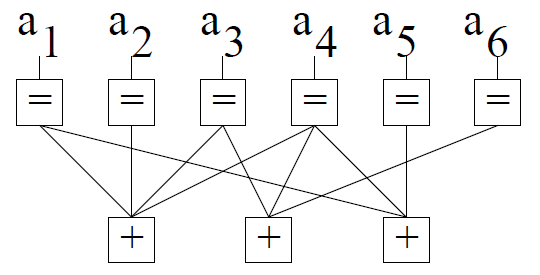
\includegraphics[width=150pt]{ldpc.png}
		\caption{Bipartitný graf reprezentujúci $(6,3)$-LDPC kód.}
	\end{figure}
	
	Majme kód reprezentovaný grafom vyššie.
	
	Kontrolnú maticu zostrojíme tak, že každý~$+$ vrchol bude reprezentovaný
	jedným riadkom, pričom tam bude $1$~pre každý $=$ vrchol, s~ktorým
	je tento $+$~vrchol spojený, $0$~pre ostatné.
	
	Pre kód zadaný daným grafom teda vyzerá kontrolná matica nasledovne:
	\[
		H =
		\begin{pmatrix}
			1 & 1 & 1 & 1 & 0 & 0 \\
			0 & 0 & 1 & 1 & 0 & 1 \\
			1 & 0 & 0 & 1 & 1 & 0 \\
		\end{pmatrix}
	\]
	
	Pre všetky slová tohto kódu potom platia nasledovné rovnosti:
	\[
		\begin{aligned} 
			a_1 + a_2 + a_3 + a_4 &= 0 \\
			a_3 + a_4 + a_6 &= 0 \\
			a_1 + a_4 + a_5 &= 0
		\end{aligned}
	\]
	
	Keď teda s použitím daného kódu obdržíme slovo $?01?11$, tak
	z~druhej rovnice vyplýva, že $a_4$~musí byť~$0$. Potom z~tretej
	rovnice vyplýva, že $a_1$~musí byť~$1$.
\end{example}


\subsection{Symetrická kryptografia}

V~symetrickej kryptografii obe strane zdieľajú jeden spoločný
tajný kľúč.

\begin{example}
	Príkladom je Caesarova šifra (posun každého písmena o konstantu).
	
	Nech Alica a Bob zdieľajú tajný kľúč $K=17$. Alica chce zakódovať 
	správu $m=\verb|INFORMATIKA JE SUPER|$. Zakódovaná správa po zakódovaní
	s~kľúčom $K=17$	bude $c=e_K(m)=\verb|ZEWFIDRKZBR AV JLGVI|$.
	
	Eva bez znalosti tajného kľúča nebude vedieť túto správu dekódovať
	(aj keď samozrejme Caesarova šifra môže mať najviac 26 rôznych kľúčov
	takže celkom jednoducho môže všetky vyskúšať). Bob so znalosťou 
	kľúča~$K$ jednoducho správu rozlúšti $m=d_K(c)$.
\end{example}

Ďalšími príkladmi sú Vigenèrova šifra (posun $n$-tic písmen, každé o různou konstantu).
Hillův kryptosystém (kódujeme $n$-tice násobením maticí-klíčem,
dekódujeme její inverzí). DES a AES.

Pre symetrickú kryptografiu by mali platiť nasledovné podmienky:
\begin{enumerate}
	\item So znalosťou kľúča~$K$ a funkcii~$e,d$ je ľahké spočítať
	$e_K(m)$ a $d_K(c)$.
	\item Zakódované $e_K(m)$ by nemalo byť o~moc dlhšie ako $m$.
	\item Malo by byť nemožné efektívne spočítať $d_K(c)$ bez znalosti
	funkcie~$d$ a kľúča~$K$.
	\item Malá zmena $m$ veľmi zmení $e_K(m)$.
	\item Množina kľúčov by mala byť veľká.
\end{enumerate}

Takisto by mali platiť podmienky \verb|CIAAN|:
\begin{itemize}
	\item \textsc{Confidentiality}: dáta môže dekódovať iba ten, 
	komu su určené
	\item \textsc{Integrity}: adresát si môže overiť, že dáta neboli 
	neautorizovane zmenené
	\item \textsc{Availability}: autorizovaní užívatelia musia mať
	prístup k~dátam a službám
	\item \textsc{Authenticity}: dáta pochádzajú od toho, od koho majú
	\item \textsc{Non-Repudiation}
\end{itemize}

Šifry sa dajú deliť na dva druhy - substitučné a transpozičné.

Substitučné nahradia časť textu časťou nejakého iného kryptotextu
podľa daných pravidiel. Môžu byť jednoduché (vždy na jedinom znaku),
monoalfabetické (zadané nejakou pevnou permutáciou),
polyalfabetické (môžu používať iné permutácie v~inej časti textu),
či polygrafické (menia naraz viac znakov).

Transpozičné šifry nemenia znaky, iba menia ich poradie v slove.

\begin{example}[Afinný kryptosystém]
	Afinný kryptosystém je špecifikovaný dvomi číslami $0 \leq a,b \leq 25$,
	$\gcd(a,26)=1$. Každý znak $x$ slova $m$ sa zakóduje ako $e_{a,b}(x)=(ax+b)\mod 26$.
	Dekóduje sa potom $d_{a,b}(y) = a^{-1}(y-b)\mod 26$.
\end{example}

\subsection{DES a AES}

DES rozdělí zprávu do 64-bitových bloků
a v~šestnácti krocích provádí nad každým blokem operace, které mají jako
argument také zvolený klíč. Argumentem operací může být i hodnota
předchozích bloků. Dešifrování spočívá v~pouhém obrácení pořadí operací.
8 bitů z~64 v~klíči je pro kontrolu parity, klíče jsou tedy prakticky
jen 56bitové.

DES byl nahrazen AES (ve verzi Rijndael [réndál]), který pracuje se
128bitovými bloky a až 256bitovými klíči. Dnes se používá například
k~šifrování disků nebo VPN.

Při šifrování AES používá matici $4 \times 4$ bytů a aplikuje na ni
postupně transformace (pro 256bitové klíče až 14 kol).
Jeden typ transformací jsou substituční tabulky,
další je posun bitů v řádcích,
ještě další je přehazování sloupců
a poslední je xor-ování sloupců s~klíčem.

\subsection{Asymetrická kryptografia}

V~kryptosystémech s~veřejným klíčem disponuje každý účastník dvěma
klíči: veřejným a soukromým. Uživatel může podepsat dokument svým
soukromým klíčem a každý potom může pomocí veřejného klíče ověřit
autenticitu dokumentu. Navíc každý může zašifrovat pomocí veřejného
klíče dokument, ten je pak dešifrovatelný pouze s~klíčem privátním.

\subsubsection{RSA}

Nejznámější kryptosystém s~veřejným klíčem je RSA, který je založený na
myšlence, že násobení čísel je snadné, zatímco na rozklad na prvočísla
dobrý algoritmus neznáme.

Pro ustanovení klíčů uživatel vygeneruje $s$-bitová prvočísla $p,q$
(typicky $s = 1024$), spočte $n = pq, \varphi(n) = (p-1)(q-1)$,
vybere velké $d$ tak, že $gcd(n, \varphi(n)) = 1$
a spočte $e = d^{-1} \mod \varphi(n)$. Veřejný klíč je tvořen dvojicí
$(n, e)$, soukromý klíč trojicí $p,q,d$.

Šifrujeme slowo $w$ výpočtem $c = w^e \bmod n$,
dešifrujeme $w = c^d \bmod n$.
Pro důkaz korektnosti potřebujeme Eulerovu větu $a^{\varphi(n)} = 1
\bmod \varphi(n)$ ($a,n$ jsou nesoudělná)
a Fermatovu větu $w^{p-1} = 1 \bmod p$ ($p$ je prvočíslo).
Pokud $p \nmid w, q \nmid w$, potom $gcd(n,w) = 1$, takže lze použít
Eulerovu větu a $c^d = w^{ed} = w^{j \varphi(n) + 1} = w \bmod n$.
Pokud $p \mid w$, ale $q \nmid w$,
pak snadno platí $w^{ed} = w \bmod p$
a navíc z~Fermatovy věty $w^{q-1} = 1 \bmod q$,
tedy
$w^{ed} = w^{ed - 1} w = w^{k(q-1)} w = (w^{q-1})^k w = 1^kw = w \bmod q$
a nakonec z Čínské zbytkové věty
$w^{ed} = w \bmod pq$.
Obě $p,q$ nemůžou dělit $w$, protože volíme čísla tak, aby $w < n$.

Prakticky zprávy kódujeme jako decimálně zapsané čísla,
rozdělené na bloky délky $i$ t.ž. $10^{i-1} \leq n < 10^i$.
Pro výpočet $w^e$ použijeme algoritmus binárního umocňování ({\em
exponentiation by squaring}).
Pro výpočet $d^{-1}$ použijeme rozšířený Euklidův
algoritmus.

% https://en.wikipedia.org/wiki/RSA_(cryptosystem)#Proofs_of_correctness

\subsubsection{Iné asymetrické kryptosystémy}
{\em Rabinov kryptosystém} je založený na tom, že modulo $n=pq$ je ľahké urobiť druhú
mocninu čísla, avšak odmocniť číslo je ťažké bez faktorizácie. Po odmocnení
vyjdú štyri odmocniny daného čísla, z~ktorých jedna je pôvodné slovo.

{\em Kryptosystém El~Gamal} je založený na diskrétnom logaritme. 
Verejným kľúčom je trojica $p,q,y$, kde $p$~je prvočíslo, $q$~je 
primitívny prvok $\mathbb{Z}^*_p$ a $y=q^x \mod p$. Súkromným kľúčom
je číslo $x < p$.

Slovo $w$ sa zakóduje pomocou náhodného čísla $r$ ako $a=q^r \mod p$,
$b=y^r w \mod p$. Kryptotextom je dvojica $(a,b)$.

Dekrypcia prebieha ako $w = \frac{b}{a^x}=ba^{-x}\mod p$.

\subsection{Kryptografie na eliptických křivkách}

Výhodou eliptických křivek je,
že pro zaručení stejné bezpečnosti jako použití běžných struktur (např.
$\mathbb{Z}_n$) stačí použít podstatně menších klíčů.

Eliptická křivka je graf bodů v~rovině splňujících
$y^2 = x + ax + b \bmod n$, kde $a,b,n$ jsou celá čísla,
spolu s {\em bodem v nekonečnu}. Uvažujeme pouze křivky, kde neexistují
násobné kořeny (ekvivalentně $4a^3 + 27b^2 \neq 0$).

Pro každou křivku můžeme definovat sčítání tak, aby body spolu se
sčítáním tvořili komutativní grupu. Vzorce jsou poměrně komplikované,
příklad sčítání poskytne obrázek. Pomocí této grupy můžeme implementovat
například RSA.

\begin{figure}[H]
    \centering
    \includegraphics[width=200pt]{ec_add.png}
    \caption{Sčítání, \href{https://www.certicom.com/content/certicom/en/21-elliptic-curve-addition-a-geometric-approach.html}{zdroj}}
\end{figure}

Výhoda, kterou eliptické křivky poskytují, je v~podstatně složitějším
hádání klíčů, tedy stačí podstatně kratší klíče pro zajištění stejné
bezpečnosti jako u standradních postupů. Stejně jako pro čísla
pro křivky není známý rychlý
způsob výpočtu diskrétního logaritmu (tedy hledání $k$ takového, že $B =
kA$).

Nevýhodou je, že pro každé $x$ nemusí existovat $y$ a tedy některé
zprávy nejdou přímo zakódovat. Problém se řeší randomizovaným
algoritmem, který přidává několik bitů za takové zprávy.

\subsection{Schémata pro digitální podpisy}

Máme zprávu $m$, její hash $h(m)$. Chceme {\em podepsat} $h(m)$ (kvůli
efektivitě ne přímo $m$) funkcí $sig_{k_s}$ závislou na páru klíčů $(k_s,
k_p)$ a ověřit podpis funkcí $ver_{k_p}$.

Jedním schématem je \uv{obrácené RSA}. V~běžném RSA máme veřejné $n = pq$,
exponent $e$ a soukromý dešifrovací exponent $d$ a čísla $p,q$.
Šifrujeme zprávu $w$: $c = w^e$. Dešifrujeme $c$: $w = c^d$.
Podpis pomocí RSA se vytvoří $c = w^d$ a ověřuje se zda $w = c^e$.

Další schémata jsou například ElGamal či Rabinovo schéma.

\subsubsection{DSA}

Ako štandard pre podpisy bol vybraný DSA, ktorý vznikol modifikáciou
podpisov pomocou schématu El Gamal. Verejným kľúčom
je štvorica $(p,q,r,y)$, kde $p$ je prvočíslo, $q$ je prvočíslo, ktoré
delí $p-1$, $r=h^{(p-1)/q}\mod p$, kde $h$ je náhodný primitívny
prvok $\mathbb{Z}_p$, $r>1$ a $y=r^x\mod p$. Privátnym kľúčom
je hodnota $x$.

Podpis slova $w$ prebieha nasledovne: vyberie sa náhodné $k < q$.
Spočíta sa $a=(r^k\mod p) \mod q$, $b = k^{-1}(w+xa)\mod q$.
Podpisom je dvojica $(a,b)$.

Podpis sa overí tak, že sa spočíta $z=b^{-1}\mod q$, $u_1=wz\mod q$,
$u_2=az\mod q$. Potom sa overí, že $r^{u_1}y^{u_2}\mod q=a$.

\subsubsection{Fiat-Shamir}
V protokole Fiat-Shamir sa pre prvočísla $p,q$ spočíta $p \cdot q = n$,
ako verejný kľúč sa vyberú čísla $v_1, \ldots, v_k$ a ako súkromný kľúč
$s_1, \ldots, s_k$, $s_i=\sqrt{v_i^{-1}}\mod n$.

Podpis a overenie TODO

\subsection{Autentizační protokoly}

(Uvedeme jeden protokol. Profesor Gruska uvádí ještě dva, technicky
náročné protokoly jejichž memorování asi nemá větší význam.)

\begin{example}
Předpokládejme, že Alice a Bob sdíli tajný klíč $k$ a jednosměrnou
funkci $f_k$. Bob pošle Alici náhodné číslo $r$, Alice pošle Bobovi
$p = f_k(r)$ (tady by se Eva mohla pokusit o podvod posláním špatného
$p$), Bob ověří $p = f_k(r)$.
\end{example}

\subsection{Protokoly pro coin tossing}

{\em Házení mincí} je způsob digitálního hození mincí takový, že ani
jedna ze dvou stran nemůže výsledek určit, ale obě strany mohou hodnotu
ověřit.

Uvedeme dva protokoly. V~tom prvním Alice vybere jednosměrnou funkci $f$
a pošle Bobovi $f(0), f(1)$. Bob se pokusí uhádnout, které z $f(0), f(1)$
je výsledkem aplikace $f$ na $1$. Alice mu sdělí, zda je jeho odpověď
správná a pošle mu $f$, aby si mohl výsledek sám ověřit.

V tom druhém Alice vybere prvočísla $p,q$, pošle Bobovi $n = pq$.
Bob vybere $1 \leq x \leq n/2$, pošle alici $y = x^2 \bmod n$.
Alice vypočte všechny čtyři kořeny $x_1, n-x_1, x_2, n - x_2$ (spočte
nějakým algoritmem nebo zkusí možnosti modulo každé prvočíslo a pak použije CRT)
a tipem vybere jeden ze dvou,
které jsou menší než $n/2$.
Alica Bobovi nepošle svoj tip, ale dá mu vedieť, ktoré si vybrala (napr. 
vyberie nejaký bit, kde sa líšia, a pošle Bobovi poradie a hodnotu 
daného bitu).
Bob jí sdělí, zda trefila $x$ nebo ne a
pošle jí ho pro ověření, zatímco ona jemu pošle $p,q$ pro ověření.


\subsection{Protokoly pro bit commitment}

Účelem protokolů pro {\em závázní se k~bitu} je provedení volby, která
nelze jiným účastníkem předčasně odhalit, ale je možné ji po odhalení
ověřit.

Například Alice může bit napsat na papírek, umístit ho do truhly, tu
zamčít a dát Bobovi. Ve chvíli odhalení pak zkontroluje integritu truhly
a odemče ji svým klíčem.  Formálněji Alice zvolí jednosměrnou funkci
$f$, sudé (liché) $x$, pokud chce zakódovat $0$ ($1$) a pošle Bobovi
$(f, f(x))$.

U protokolů popisujeme {\em commitment phase} a {\em opening phase}.
Od protokolů očekáváme tři vlastnosti:
\begin{itemize}
    \item {\em hiding} -- Bob nemůže volbu Alice odhalit,
    \item {\em binding} -- Alice nemůže volbu skrytě změnit,
    \item {\em correctness} -- pokud vše probíhá dle protokolu, Bob se dozví správný bit.
\end{itemize}

Další protokol je například následující. Mějme prvočísla $p,q$,
číslo $n = pq$ a nakonec $m$ je kvandratický nezbytek\footnote{Tedy
neexistuje $x$ takové, že $x \bmod n = m$.} modulo $n$. Čísla $n, m$
zveřejníme.  Commitment je potom $f(b, x) = m^b x^2 \bmod n$ pro náhodně
zvolené $x \in \mathbb{Z}^*_n$. Protokol je hiding, protože výpočet
kvadratických zbytků je těžký. Protokol je binding, protože $m \in
QNR(n)$, a proto neexistují $x_1, x_2$ takové, že
$m x_1^2 = x_2^2 \bmod n$.


\subsection{Protokoly pro oblivious transfer}

Problém: Navrhnout protokol, který pošle zprávu od Alice Bobovi tak, že
Bob ji dostane s~pravděpodobností $1/2$. Bob ví, zda dostal zprávu nebo
chybnou zprávu, Alice to nezjistí.

Takový je například následující protokol:
\begin{enumerate}
    \item Alice zvolí dvě prvočísla $p,q$ a pošle Bobovi $n = pq$.
    \item Bob zvolí náhodně $x$ a pošle $y = x^2 \bmod n$.
    \item Alice spočte čtyři kořeny $y \bmod n$ a pošle jeden z~nich
        Bobovi.
    \item Bob ověří, jestli zaslaný kořen je kongruentní $x$. Pokud ano,
        nic se nedozvěděl. Pokud ne, má dva různé kořeny modulo $n$ a
        může tak faktorizovat $n$. Alice se nic nedozvěděla.
\end{enumerate}

Můžeme také navrhnout protokol, ve kterém Alice pošle dvě zprávy a Bob
se dozví právě jednu z~nich a Alice se nedozví kterou.

\subsection{Steganografie a vodotisk}

Steganografie skrývá hlavní zprávu v~datech (například jako tajný přenos
dat), zatímco vodotisk je pouze
značkou umístěnou do hlavní zprávy (například pro kontrolu původu).

\begin{verbatim}
Příkladem,
a to ne moc dobrým,
steganografie v textu je
tento
asymetrický odstavec.
\end{verbatim}

Existují algoritmy pro vložení bitů do obrázků (jejich popis je
technický).

K digitálnímu vodotisku profesor Gruska říká pouze tolik, že jde o
vložení značky do dat tak, aby nešla odstranit nebo nejlépe ani
detekovat. Schmématem (bez bližšího vysvětlení) znázorňuje jak probíhá
vložení značky a její extrakce pro ověření. Rozlišuje míru znalostí pro
ověření: buď je potřeba originálu dat i verze s vodotiskem, nebo stačí
mít verzi s~vodotiskem.

% https://www.fi.muni.cz/usr/gruska/crypto17/cr1711.pdf

\subsection{Kryptografické stroje a jejich historie}

V~histórii kryptografie hovoríme o~štyroch obdobiach:
\begin{enumerate}
	\item Kryptografia bez strojov: lingvistické šifry (Caesar, Vigenère, Hill)
	\item Mechanická kryptografia: napr. Enigma
	\item Digitálna kryptografia: počítače, RSA, DSA, AES, ...
	\item Kvantová kryptografia
\end{enumerate}

Enigma byla vynalezena v~roce 1918. Má tři libovolně rotory, kde každá
pozice implementuje Caesarovu šifru. První rotor po napsání písmena
otočí o jedno dál a až obejde celou otáčku, tak posune o jedna další
rotor.  Navíc má Enigma desku pro transpozici písmen. Dohromady asi
$10^{16}$ možných konfigurací.

V~roce 1931 se dostaly do Francie dokumenty popisující zapojení rotorů.
Tento popis se dostal do rukou matematikovi Rejewskému,
který s~chytrým využitím teorie grup dokázal shrnout problém hledání
konfigurace Enigmy do několika rovnic.
Rejewski si navíc všiml, že Němci na začátku dne pro kontrolu dvakrát pošlou jednu
třípísmennou zprávu, což umožnilo redukovat počet možností pro kód
zvolený Němci pro daný den.

Rejewski měl k~dispozici model Enigmy pro komerční použití se zapojením
kláves v~běžném pořadí německých psacích strojů, $QWERTZU$\ldots Enigma
pro vojenské účely však měla klávesy v~pořadí $ABCDEF$\ldots -- tuto
možnost Britští kryptoanalytici ani nevyzkoušeli, jelikož ji považovali
za příliš zřejmou.

Rejewského tým navrhl mechanický počítač Bomba, který zkoušel již značně
omezený počet kombinací, což umožnilo dešifrovat zprávy z~Enigmy každý
den. Tuto technologii předali pět týdnu před začátkem války Francouzům a
Britům. Britský tým tuto technologii značně zdokonalil.

\subsection{Kvantová kryptografie}

Ve slidech profesora Grusky (které na přednášce neprobral)
a na Wikipedii.
% https://en.wikipedia.org/wiki/Quantum_key_distribution
% https://en.wikipedia.org/wiki/Quantum_teleportation

Pokúsim sa to tu nejako popísať, avšak za správnosť a úplnosť informácií
neručím.

Kvantová kryptografia je teoreticky absolútne bezpečná, fyzikálne
zákonu zaručujú, že sa (v~istých prípadoch) nedá prelomiť. Kvantová
informácia sa ťažko ukladá a posiela, nie je možné ju skopírovať
a meraním sa zničí. Tento fakt prakticky znemožňuje man-in-the-middle
útoky, keďže pokiaľ by útočník informáciu získal, táto sa zničila
a on nie je schopný ju poslať ďalej; komunikujúce strany sa teda 
dozvedia o~útočníkovi. Kvôli tomuto v~kvantovej kryptografii
neexistuje spôsob ako vykonávať bit commitment a oblivious transfer.

V~kvantových počítačoch je informácia reprezentovaná qubitmi,
ktoré môžu mať ľubovoľnú z~nespočetného množstva hodnôt 
$\alpha|0\rangle + \beta|1\rangle$, kde $|\alpha|^2+|\beta|^2=1$ a 
$|\phi\rangle$ je stĺpcový vektor ekvivalentný $\phi$.

Qubit register môže mať naraz uložené všetky superpozície $2^n$.

\subsubsection{Generování náhodných tajných klasických klíčů}
Cieľom je využiť metód kvantovej kryptografie na vygenerovanie
náhodného tajného kľúča, ktorý bude mať Alica aj Bob, a Eva
nebude mať šancu ho zistiť.

Alica vygeneruje náhodný kľúč a posiela ho Bobovi nasledovne:
pre každý znak si vyberie náhodne bázu ($|0\rangle$, $|0'\rangle$,
resp. $|1\rangle$, $|1'\rangle$) a túto informáciu pošle Bobovi.

Bob prichádzajúce fotóny meria náhodne buď so štandardnou bázou~B
alebo s~duálnou bázou~D.

Pokiaľ meria s~bázou~B a Alica poslala buď $|0\rangle$ alebo $|1\rangle$,
Bob obdrží správnu hodnotu s~pravdepodobnosťou~1, inak je hodnota,
ktorú obdrží, dokonale náhodná.

Bob potom Alici pošle (klasickým kanálom) postupnosť báz, ktorú použil 
na meranie. Alica mu potom povie, ktoré bázy vybral správne,
a tieto hodnoty sú potom vybrané ako kľúč.

\begin{example}
	Alica posiela postupnosť \verb|10001100011| a posiela ju polarizovanú
	ako $|1\rangle|0'\rangle|0\rangle|0'\rangle|1\rangle|1'\rangle|0'\rangle|0\rangle|0\rangle|1\rangle|1'\rangle$.
	Bob použije na meranie postupnosť báz \verb|BDDDBBDBBDB| a obdrží
	postupnosť \verb|10001000010|.
	Po komunikácii klasickým kanálom vie, že obdržal postupnosť \verb|10R01R000RR|
	a kľúčom sa teda stáva postupnosť \verb|1001000|.
\end{example}

\subsubsection{Kvantová teleportace}
Princípom je, že Alica a Bob zdieľajú dve častice, ktoré
sú kvantovo prepojené.
\[
	|EPR_{pair}\rangle=\frac{1}{\sqrt{2}}(|00\rangle+|11\rangle)
\]
Potom stačí odmerať jednu z~častíc a meranie druhej častice je známe.
Toto sa dá využiť napríklad na zdieľanie symetrického kľúča.

\section{Matematická analýza}

\subsection{Úvod}
Okrem učiva predmetu \verb|MA002| Matematická analýza by asi bolo
vhodné vedieť aj základy, najmä definície, tj. učivo predmetov
\verb|MB102/MB202| Diferenciální a integrální počet a 
\verb|MB103/MB203| Spojité modely a statistika.

\subsubsection*{Znenie otázky}
Matematická analýza. Systémy lineárních diferenciálních rovnic a 
metody jejich řešení; křivkový integrál.

\subsubsection*{Pojmy}
Diferenciálna rovnica, DR 1. rádu (separovateľná, lineárna homogénna,
lin. nehomogénna), Bernoulliho DR, LDR vyšších rádov, použitie DR;
krivkový integrál, krivka (jednoduchá, uzavretá, Jordanova), 
ekvivalentné krivky, súčet kriviek, opačná krivka, rozdiel kriviek,
derivácia krivky, dotyčnica, hladká krivka, orientácia krivky,
dĺžka krivky, krivkový integrál I. druhu + výpočet, krivkový
integrál II. druhu + výpočet, použitie krivkového integrálu,
Greenova veta.

\subsection{Základy}
{\em Postupnosť} reálnych čísel je zobrazenie $a: \mathbb{N} \to \mathbb{R}$,
ktorej prvky sa značia~$a_i$. Ľubovoľný interval obsahujúci 
bod~$x_0 \in \mathbb{R}$ sa nazýva okolím bodu~$x_0$ a značí~$\mathcal{O}(x_0)$.
Inteval $(A, \infty)$ (resp. $(-\infty, A)$) pre nejaké $A \in \mathbb{R}$
sa nazýva okolím bodu~$\infty$ (resp.~$-\infty$). Špeciálnymi prípadmi
je $\delta$-okolie bodu $\mathcal{O}_{\delta}(x_0)=(x_0 - \delta, x_0 + \delta)$,
prestencové okolie $\mathcal{P}(x_0)$, ktoré neobsahuje samotný bod, ľavé a pravé okolia.

\begin{definition}[Limita]
	{\em Limita} postupnosti sa pomocou okolia definuje nasledovne:
	\[
		\lim_{n \to \infty} a_n = a \in \mathbb{R}^*: \forall \mathcal{O}(a)~\exists n_0 \in \mathbb{N}~\forall n \geq n_0: a_n \in \mathcal{O}(a).
	\]

	Funkcia $f$ má {\em limitu} v bode $x_0 \in \mathbb{R}^*$ rovnú
	$L \in \mathbb{R}^*$, pokiaľ $\forall \epsilon > 0~\exists \delta > 0$
	také, že $\forall x \in mathcal{P}_{\delta}(x_0)$ platí
	$|f(x) - L| < \epsilon$.
	
	Limita sa nazýva {\em nevlastnou}, pokiaľ $L = \pm \infty$, 
	{\em vlastnou} inak. Je {\em limitou v~nevlastnom bode}, pokiaľ
	$x_0 = \pm \infty$, inak je {\em limitou vo~vlastnom bode}.
	
	{\em Limita zprava} (resp. {\em limita zľava}) sa definuje jednoducho
	nahradením okolia bodu~$x_0$ príslušným jednostranným okolím.
\end {definition}

\begin{definition}[Derivácia]
	Funkcia~$f$ má {\em deriváciu} vo~vnútornom bode $x_0$ rovnú danej 
	limite, pokiaľ existuje
	\[
		f'(x_0) = \lim_{x \to x_0} \frac{f(x)-f(x_0)}{x-x_0}.
	\]
	
	Pokiaľ je táto derivácia rovná $\pm \infty$, hovoríme
	o~{\em nevlastnej} derivácii, inak o~{\em vlastnej}.
	
	Ak má funkcia deriváciu v~každom bode nejakého intervalu,
	funkcia $f'$ sa nazýva {\em deriváciou} funkcie $f$.
\end{definition}

\begin{theorem}[L'Hospitalovo pravidlo]
	Nech $x_0 \in \mathbb{R}^*$ a nech je splnená jedna z~podmienok
	\begin{enumerate}
		\item $\lim_{x \to x_0}f(x) = \lim_{x \to x_0}g(x) = 0$,
		\item $\lim_{x \to x_0}g(x)=\pm\infty$
	\end{enumerate}
	Potom platí
	\[
		\lim_{x \to x_0}\frac{f(x)}{g(x)} = \lim_{x \to x_0}\frac{f'(x)}{g'(x)},
	\]
	pokiaľ druhá limita existuje. Ak druhá limita existuje, existuje aj prvá.
\end{theorem}

\begin{definition}[Prírastok]
	Nech je funkcia $f$ definovaná v~$\mathcal{O}(x_0)$ a pre 
	$h \in \mathbb{R}$ platí $x_0 + h \in \mathcal{O}(x_0)$.
	Potom číslo $h$ nazývame {\em prírastok nezávisle premennej}
	a $\Delta f(x_0)=f(x_0+h)-f(x_0)$ nazývame {\em prírastok 
	závisle premennej}.
\end{definition}

\begin{definition}[Diferenciál]
	Funkcia~$f$ je {\em diferencovateľná} v bode~$x_0 \in \mathbb{R}$,
	pokiaľ existuje $\mathcal{O}(x_0)$ také, že
	\[
		f(x_0+h)-f(x_0)=A \cdot h + \tau(h),
	\]
	kde $A \in \mathbb{R}$ je vhodné číslo a $\tau(h)$ je funkcia taká, že
	\[
		\lim_{h \to 0} \frac{\tau(h)}{h} = 0.
	\]
	Ak je $f$ v $x_0$ diferencovateľná, výraz $A \cdot h$ sa nazýva 
	{\em diferenciál} funkcie~$f$ a značí $\partial f(x_0)$.
\end{definition}

\begin{theorem}[Eulerova identita]
	\[
		\cos(\varphi) + i \sin(\varphi) = e^{i \varphi}
	\]
\end{theorem}

\begin{definition}[Neurčitý integrál]
	Funkcia~$F$ je na intervale~$I$ {\em primitívnou funkciou}
	funkcie~$f$, pokiaľ pre všetky $x \in I$ platí $F'(x)=f(x)$.
	
	Množina primitívnych funkcií k~funkcii~$f$ sa nazýva 
	{\em neurčitý integrál} funkcie~$f$ a značí sa $\int f(x) dx$.
\end{definition}

\begin{theorem}[Metóda per partes]
	\[
		\int uv' dx = uv - \int u'v dx
	\]
\end{theorem}

\begin{example}
	\[
		\int x \sin x dx = 
		\left|{\begin{array}{cc}
		  u=x & u'=1 \\
		  v'=\sin x & v = -\cos x
		  \end{array} } \right|
	\]
	\[
		= x \cdot (-\cos x) - \int 1 \cdot (-\cos x)dx = -x \cos x + \int \cos x dx = -x \cos x + \sin x + c
	\]
\end{example}

\begin{theorem}[Substitučná metóda]
	\[
		\int f(\varphi(x))\varphi'(x) dx =
		\left|{\begin{array}{c}
		  t = \varphi(x) \\
		  dt = \varphi'(x)dx
		  \end{array} } \right|
		= \int f(t) dt 
	\]
	\[
		\int f(x) dx  =
		\left|{\begin{array}{c}
		  x = \varphi(t) \\
		  dx = \varphi'(t)dt
		  \end{array} } \right|
		= \int f(\varphi(t))\varphi'(t) dt 
	\]
\end{theorem}

\begin{example}
	\[
		\int x e^{x^2} dx = 
		\left|{\begin{array}{c}
		  t = x^2 \\
		  dt = 2x dx \\
		  \frac{1}{2} dt = x dx
		  \end{array} } \right|
		  = \int e^t \frac{1}{2} dt = \frac{1}{2} e^t + c = \frac{1}{2} e^{x^2} + c
	\]
\end{example}

\begin{definition}[Riemannov integrál]
	Nech funkcia~$f$ je ohraničená na intervale $[a,b]$, $D=\{x_0, \cdots, x_n \}$
	je delenie intervalu $[a,b]$. Potom nech $m_i=\inf{\{ f(x) | x \in [x_{i-1},x_i] \}}$
	a $M_i=\sup{\{ f(x) | x \in [x_{i-1},x_i] \}}$.
	
	{\em Dolný súčet} príslušný deleniu $D$ je $s(D,f)=\sum_{i=1}^n m_i(x_i-x_{i-1}$
	a {\em horný súčet} príslušný deleniu $D$ je $S(D,f)=\sum_{i=1}^n M_i(x_i-x_{i-1}$.
	
	Nech $\mathcal{D}$ je množina všetkých delení intervalu $[a,b]$. Potom
	{\em dolný Riemannov integrál} funkcie~$f$ na intervale $[a,b]$ je
	\[
		\int_{\overline{a}}^b f(x) dx = \sup \{ s(D,f) | D \in \mathcal{D} \}.
	\]
	{\em Horný Riemannov integrál} funkcie~$f$ na intervale $[a,b]$ je
	\[
		\int_a^{\underline{b}} f(x) dx = \inf \{ S(D,f) | D \in \mathcal{D} \}.
	\]
	
	Pokiaľ sa tieto integrály rovnajú, tak táto funkcia je na intervale $[a,b]$
	{\em Riemannovsky integrovateľná} a 
	\[
		\int_a^b f(x) dx = \int_{\overline{a}}^b f(x) dx = \int_a^{\underline{b}} f(x) dx.
	\]
\end{definition}

\begin{theorem}[Newton-Leibnitzov vzorec]
	Nech funkcia~$f$ je integrovateľná na intervale $[a,b]$ a funkcia~$F$
	je k~nej primitívna na danom intervale, tj. $F'=f$. Potom platí
	\[
		\int_a^b f(x) dx = F(b) - F(a).
	\]
\end{theorem}

\begin{example}
	\[
		\int_{-2}^5 x^2 dx = \left[ \frac{x^3}{3} \right]_{-2}^5 = \frac{5^3}{3} - \frac{(-2)^3}{3} = \frac{133}{3}
	\]
\end{example}

\begin{definition}[Nevlastný integrál]
	Nech funkcia~$f$ je definovaná na intervale $[a,\infty)$ a na
	každom intervale $[a,b]$, kde $b > a$ je integrovateľná. 
	Funkciu~$F$ na intervale $[a, \infty)$ definujme ako 
	$F(b) = \int_a^b f(x) dx$. 
	
	Ak existuje vlastná limita $\lim_{b \to \infty} F(b)$, hovoríme
	že nevlastný integrál konverguje a kladieme
	\[
		\int_a^{\infty} f(x) dx = \lim_{b \to \infty} F(b) = \lim_{b \to \infty} \int_a^b f(x) dx.
	\]
	
	Ak táto vlastná limita neexistuje, hovoríme, že integrál diverguje.
	Pokiaľ existuje nevlastná limita, hovoríme, že určite diverguje,
	inak osciluje.
\end{definition}

Rovnako sa dá definovať nevlastný integrál z~druhej strany.

\subsection{Obyčejné diferenciální rovnice}

\begin{definition}
Nechť $x$ je proměnná, $y$ je funkce proměnné $x$, $y' = \dv{y}{x}$.
Na $y, y'$ můžeme nahlížet také jako na {\em závislé proměnné}
v $\mathbb{R}$. Nechť $F : M \subseteq \mathbb{R}^3 \to \mathbb{R}$
je daná funkce. Pak rovnice
\[
    F(x,y,y') = 0
\]
se nazývá {\em obyčejná diferenciální rovnice prvního řádu}.

{\em Řešení} takové rovnice je každá funkce $\varphi(x) = y$,
která má derivaci na intervalu $\mathcal{I} \subseteq \mathbb{R}$,
a platí $[x, \varphi(x), \varphi'(x)] \subseteq M$
a $\forall x \in \mathcal{I} \; F(x, \varphi(x), \varphi'(x)) = 0$.
\end{definition}

\begin{example}[Se separovatelnými proměnnými]
Rovnice tvaru $y' = g(x) h(y)$. Například následující.
\begin{align*}
    2 y'             &=    2x + 1               \\
    2 \dv{y}{x}      &=    2x + 1               \\
    2 \; \text{d}y   &=   (2x + 1) \; \text{d}x \\
    \int 2 \; \text{d}y &= \int (2x + 1) \; \text{d}x \\
    2 y              &= x^2 + x +C               \\
      y              &= \frac{x^2 + x + C}{2}    \\
\end{align*}
\end{example}

\begin{example}[Lineární rovnice]
    % http://people.math.gatech.edu/~xchen/teach/ode/nth_ord_eq.pdf
    Rovnice tvaru $y' + p(x)y = q(x)$.
    Řešení homogenní varianty takové rovnice (tj. $y' + p(x)y = 0$)
    jsou tvaru $e^{\int -p(x) \; \text{d}x}$.
    Úpravami se pak snadno získá řešení homogenní varianty a z něj pak
    dosazením původní rovnice.
    Například následující.
\begin{align*}
    y' + 2xy        &= x \\
    \text{Nejprve vyřešíme } y' + 2xy &= 0 &\\
    y_H &= e^{\int -2x \; \text{d}x} = e^{-x^2} \cdot C(x) \\
    \text{Zpět k řešení původní rovnice;}&\text{ potřebujeme C(x) tak, aby} \\
    y'_H + 2xy_H   &= x \\
    (-2x e^{-x^2} \cdot C(x) + e^{-x^2} \cdot C'(x)) + 2x e^{-x^2}\cdot C(x) &= x \\
    e^{-x^2} C'(x) &= x \\
    C'(x) &= x e^{x^2} \\
    C(x)  &= \frac{1}{2} e^{x^2} + K \\
    \text{Zbývá dosadit }& C(x) \text{ do } y_H \\
    y &= e^{-x^2} (\frac{1}{2} e^{x^2} + K) = \frac{1}{2} + e^{-x^2} K
\end{align*}
\end{example}

\begin{example}[Bernoulliho rovnice]
    Rovnice tvaru $y' + p(x)y = q(x)y^k$. Řešíme převodem na lineární
    rovnici pomocí substituce $u = y^{1-k}$. Například následující.
\begin{align*}
    y' + y + y^2 e^x  &= 0 \\
    y' + y          &= - e^x y^2 \\
    (u = y^{1-2} = y^{-1} &\implies y = u^{-1}) \\
    (u^{-1})' + u^{-1}    &= - e^x u^{-2} \\
    -u^{-2} u' + u^{-1}   &= - e^x u^{-2} \\
    u' - u          &= e^x  \text{ (nyní řešíme lineární rovnici)}  \\
    u'_H - u        &= 0 \\
    u_H             &= e^{\int 1 \; \text{d}x} = e^x C(x) \\
    (e^{x} C(x))' - e^{x} C(x) &= e^x \\
    e^x C(x) + e^x C'(x) - e^{x} C(x) &= e^x \\
    e^x C(x) + e^x C'(x) - e^{x} C(x) &= e^x \\
    C'(x) &= 1 \\
    C(x)  &= x + K \\
    u'    &= e^x (x + K) \\
    y     &= \frac{1}{e^x (x + K)}
\end{align*}
Navíc se nezapomene ověřit možné (a skutečné) řešení $y = 0$, jelikož
výpočet pracoval s výrazem $y^{-1}$.
\end{example}

\begin{example}[Exaktní rovnice]
Rovnice tvaru
$M(x,y) \diff{x} + N(x,y) \diff{y} = 0$,
kde
$\frac{\partial M(x,y)}{\partial y} = \frac{\partial N(x,y)}{\partial x}$.
Hledáme kmenovou funkci $F(x,y)$, což je taková funkce, že
$M = \frac{\partial F}{\partial x}$, $N = \frac{\partial F}{\partial y}$.
Například následující.
\begin{align*}
    4x^3 e^y \diff{x} + (x^4e^y + 2y) \diff{y} &= 0
        \text{ (nezapomene ověřit exaktnost)} \\
    F(x,y) = \int M(x,y) \diff{x} &= x^4 e^y + C(y) \\
    \frac{\partial F}{\partial y} = x^4 e^y + C'(y) &\boldsymbol{=} x^4e^y + 2y = N
        \text{ (z exaktnosti)} \\
    C'(y)  &= 2y \\
    C(y)   &= y^2 + K \\
    F(x,y) &= e^y x^4 + y^2 + K
\end{align*}
\end{example}

\begin{example}[Lineární rovnice vyšších řádů]
    % http://people.math.gatech.edu/~xchen/teach/ode/nth_ord_eq.pdf
    Je-li rovnice tvaru
    $a_n y^{(n)} + \ldots + a_1 y' + a_0 y = 0$, tedy je
    vyššího řádu a lineární s konstantními koeficienty,
    potom se převede na {\em charakteristickou rovnici}
    $a_n \lambda^{n} + \ldots a_1 \lambda + a_0 = 0$.
    Každý kořen $\lambda$ s násobností $k$
    zadává $k$ řešení tvaru
    $e^{\lambda t},
    \ldots
    t^{k-1} e^{\lambda t}$.
    Například následující.
\begin{align*}
    y'' + 16 y &= 0 \\
    \lambda^2 + 16 &= 0 \\
    \lambda &= \pm 4i \\
    y_1 &= e^{4it} = \cos 4t + i \sin 4t \\
    y_{11} &= \cos 4t \\
    y_{12} &= \sin 4t \\
    y_2 &= e^{-4it} \text{ (úprava je stejná až na znaménko)} \\
    y  &= c_1 \cos 4t + c_2 \sin 4t
\end{align*}
\end{example}

\subsection{Systémy diferenciálních rovnic}

\begin{definition}
    Soubor $n$ rovnic tvaru
    $x'_i = \sum_{j=1}^{n} a_{i,j}(t) \cdot x_j + b_i(t)$,
    kde $a_{i,j}, b_i$ jsou reálné funkce spojité na intervalu
    $\mathcal{I}$ a $' = \dv{}{t}$,
    se nazývá {\em systém lineárních diferenciálních rovnic 1. řádu}.

    Systém rovnic lze zapsat jako
    $x' = A(t) \cdot x + b(t)$
    při zavedení značení $x(t)$, $b(t)$, $A(t)$
    pro odpovídající vektory (matici) ze soustavy
    a realizaci operací po složkách.

    {\em Řešení} je každá vektorová funkce $\varphi(t)$
    diferencovatelná na intervale $\mathcal{J} \subseteq \mathcal{I}$,
    taková, že po dosazení za $x$ v systému je systém splněn.
\end{definition}

\subsubsection{Homogenní systémy}
%\begin{theorem}
    %Jsou-li $A(t), b(t)$ spojité na intervalu $\mathcal{I}$,
    %potom $x' = A(t)x + b(t)$, $x(t_0) = \eta$
    %má pro každé $t_0 \in \mathcal{I}$ a $\eta \in \mathbb{R}^n$
    %právě jedno řešení, které existuje na celém $\mathcal{I}$.
    %Toto řešení lze vyjádřit jako limitu určité posloupnosti aproximací.
%\end{theorem}

Nechť $A(t)$ je maticová funkce řádu $n$ spojitá na $\mathcal{I}$.
Mějme homogenní systém $y' = A(t) y$.
Pokud $y_1(t)$ a $y_2(t)$ jsou řešení (tedy např. $y_1' = A(t) y_1$,
pak se snadno derivováním
ověří, že i $y(t) = c_1 y_1(t) + c_2 y_2(t)$ je řešení. Tím dostáváme
následující.

\begin{theorem}
    Množina všech řešení homogenního systému na intervalu $\mathcal{I}$
    tvoří vektorový prostor nad tělesem reálných čísel.
\end{theorem}

Navíc platí (bez důkazu), že tento vektorový prostor má dimenzi $n$.

\begin{definition}
    Libovolná báze prostoru všech řešení na intervalu $\mathcal{I}$ se
    nazývá {\em fundamentální systém řešení} rovnice $y' = A(t)y$.

\end{definition}

Pokud $y_1(t), \ldots, y_n(t)$ je fundamentální systém řešení, pak
$y(t) = c_1 y_1(t) + \ldots + c_n y_n(t)$, je {\em všeobecným
řešením} systému $y' = A(t) y$.

S vektorovou rovnicí $y' = A(t) y$ můžeme uvažovat i
{\em maticovou rovnici} $Y' = A(t) Y$.
Pokud $Y(t)$ je maticové řešení na $\mathcal{I}$
a $C \in \mathbb{R}^{n \times n}$ je konstantní matice, potom
i $Y(t) C$ je řešením. Tento fakt opět snadno ověříme derivací
$(YC)' = Y'C = AYC = A(YC)$.
Maticové řešení $Y(t)$ nazýváme {\em fundamentální matice},
pokud sloupce $Y(t)$ tvoří fundamentální systém řešení $y' = A(t)y$.
Řešení $Y(t)$ je tedy fundamentální právě tehdy, když
$det(Y) \neq 0$ pro každé $t \in \mathcal{I}$. (Navíc platí věta, která
říká, že $det(Y) = 0$ buď pro všechny $t$ nebo pro žádné.)


\begin{example}[Eliminační metoda]
Derivováním jedné z rovnic a dosazením druhé dostaneme lineární
diferenciální rovnici s konstantními koeficienty jedné proměnné.
Ten vyřešíme a dosadíme zpět. Například následující.
\begin{align*}
    x' &= 7x + 6y \\
    y' &= 2x + 6y \\
    \\
    x'' &= 7x'+6y' \\
    x'' &= 7(7x+6y) + 6(2x+6y) = 61x+78y \\
    y   &= \frac{x' - 7x}{6} \\
    x'' &= 61x + 13x' - 91x = 13x' - 30x \\
    \text{To je lineární rovnice.} \\
    x &=  c_1 e^{3t} + c_2 e^{10t} \\
    \text{Dosadíme zpět do výrazu pro } y \\
    y &= -\frac{2}{3} c_1 e^{3t} + \frac{1}{2} c_2 e^{10t} \\
    \text{Řešením je tedy}& \text{ fundamentální matice Y(t)} \\
    \text{vynásobená}& \text{ vektorem konstant.} \\
\end{align*}
\vspace{-25pt}
\[
    \begin{pmatrix}
        e^{3t} & e^{10t} \\
        -\frac{2}{3}e^{3t} & \frac{1}{2} e^{10t} \\
    \end{pmatrix}
    \begin{pmatrix}
        c_1 \\
        c_2 \\
    \end{pmatrix}
\]
\end{example}

\pagebreak

\subsubsection{Systémy s konstantními koeficienty}

\begin{definition}
    Nechť $M$ je komplexní matice řádu $n$. Pak $e^M$ nazveme
    {\em exponenciála matice} $M$.
\[
    e^M = \sum_{k = 0}^{\infty} \frac{1}{k!} M^k
\]
\end{definition}

\begin{theorem}
    Nechť $A$ je konstantní matice řádu $n$.
    Pak $e^{At}$ je fundamentální matice homogenního systému $y' = Ay$
    na $(-\infty, \infty)$.
\end{theorem}

\begin{example}
\end{example}

\subsubsection{Partikulární řešení nehomogenních systémů}

Budeme uvažovat nehomogenní systém $x' = A(t)x + b(t)$.
Připomeneme, že $A(t), b(t)$ jsou maticová a vektorová funkce,
definované a spojité na intervalu $\mathcal{I}$.

\begin{theorem}
    Nechť $Y' = A(t)Y$ a $x_0(t)$ je nějaké řešení nehomogenního systému
    na $\mathcal{I}$. Potom vektorová funkce $x(t)$ je úplné řešení
    nehomogenního systému na $\mathcal{I}$ právě tehdy,
    když pro každé $t \in \mathcal{I}$
    \[
        x(t) = Y(t)c + x_0(t)
    \]
\end{theorem}

\begin{example}
    (Metodou variace konstant.)
\end{example}

\subsection{Krivkový integrál}
\begin{definition}[Krivka]
	Nech $m \in \mathbb{N}$ a $\mathcal{I} \subseteq \mathbb{R}$
	je interval.
	{\em Krivkou} v $\mathbb{R}^m$ je každá vektorová
	funkcia $\varphi: \mathcal{I} \to \mathbb{R}^m$, 
	ktorá je na $\mathcal{I}$ spojitá.
	
	Množina $\langle \varphi \rangle = \varphi(\mathcal{I})=
	\{ \varphi(t) | t \in \mathcal{I} \} \subseteq \mathbb{R}^m$
	je {\em geometrickým obrazom (trajektóriou) krivky} $\varphi$. Funkcia~$\varphi$
	sa potom nazýva {\em parametrizáciou množiny} $\langle \varphi \rangle$.
\end{definition}

Krivka je {\em jednoduchá}, ak je na intervale $[a,b]$ prostá,
{\em uzavretá}, ak $\varphi(a)=\varphi(b)$ a {\em Jordanova}, ak
je jednoduchá a uzavretá.

\begin{definition}
	Majme krivky $\varphi: [a,b] \to \mathbb{R}^m$ a 
	$\psi : [\alpha, \beta] \to \mathbb{R}^m$. Tieto krivky
	sú {\em ekvivalentné} ($\varphi \sim \psi$), ak existuje 
	spojito diferencovateľné
	zobrazenie $w : [\alpha, \beta] \to [a,b]$ také, že
	$w'(t) \neq 0$ pre každé $t$ a platí
	$\varphi(w(t)) = \psi(t)$ pre každé $t \in [\alpha, \beta]$.
\end{definition}

\begin{definition}[Operácie na krivkách]
	Majme krivky $\varphi: [a,b] \to \mathbb{R}^m$ a 
	$\psi : [\alpha, \beta] \to \mathbb{R}^m$ také, že platí
	$\varphi(b)=\psi(\alpha)$.
	
	Ich {\em súčet} definujeme ako 
	\[
		(\varphi \oplus \psi)(t) =
		\begin{cases}
			\varphi(t) & t \in [a,b] \\
			\psi(t+\alpha-b) & t \in [b, b + \beta - \alpha]
		\end{cases}
	\]
	
	{\em Opačnú krivku} definujeme ako
	\[
		(\ominus \varphi)(t) = \varphi(-t), t \in [-b, -a].
	\]
\end{definition}

\begin{definition}[Derivácia krivky]
	Majme krivku $\varphi=(\varphi_1, \ldots, \varphi_m)$ na intervale
	$[a,b]$. Deriváciou krivky v~bode $t \in [a,b]$ je vektor
	$\varphi'(t) = (\varphi_1'(t), \ldots, \varphi_m'(t))$, pričom pre $t=a$
	a $t=b$ sa uvažujú jednostranné derivácie.
\end{definition}

\begin{definition}[Hladká krivka]
	Krivka $\varphi$ sa nazýva {\em hladká}, ak funkcia $\varphi$
	je na $[a,b]$ spojito diferencovateľná a pre každé $t \in [a,b]$
	platí $\varphi'(t) \neq 0$.
	
	Krivka je {\em po častiach hladká} ak sa dá rozdeliť na konečný 
	súčet hladkých kriviek.
\end{definition}

Orientácia krivky je nejaké usporiadanie množiny $\langle \varphi \rangle$.
Môže byť súhlasné alebo nesúhlasné s~parametrizáciou.

\begin{definition}[Delenie krivky]
	Nech $\varphi : [a,b] \to \mathbb{R}^m$ je krivka orientovaná
	súhlasne s~parametrizáciou. Uvažujme konečné delenie intervalu [a,b] také, že
	$a=t_0 < t_1 < \cdots < t_n = b$. 
	
	Body $P_i = \varphi(t_i)$ sa nazývajú {\em delením krivky} $\varphi$.
	
	Množinu $\langle \varphi \rangle$ aproximujeme lomenou čiarou~$L$
	tvorenou úsečkami medzi bodmi $P_i$. Jej dĺžka $m_1(L)$ je potom 
	súčtom dĺžok daných úsečiek.
\end{definition}

\begin{definition}[Dĺžka krivky]
	Ak existuje $M \in \mathbb{R}$ také, že pre každú lomenú čiaru~$L$
	platí $m_1(L) \leq M$, krivka $\varphi$ má konečnú dĺžku. Najmenšie 
	takéto $M$ nazývame {\em dĺžkou} krivky $\varphi$, značíme 
	$m_1(\langle \varphi \rangle)$.
\end{definition}

\begin{theorem}
	Každá regulárna krivka má konečnú dĺžku a platí
	\[
		m_1(\langle \varphi \rangle) = \int_a^b ||\varphi'(t)|| dt = \int_a^b \sqrt{(\varphi_1'(t))^2 + \cdots + (\varphi_m'(t))^2} dt
	\]
\end{theorem}

\subsubsection{Křivkový integrál I. druhu}


Křivku můžeme rozdělit na části a potom spočítat součet délek částí
vážených hodnotou funkce v~nějakém bodě každé z~částí. Pokud je
dělení takové, že nejdelší z~jeho části je v~limitě (to jest když je
dělení na $n\to \infty$ částí) délky 0, a potom posloupnost výše
popsaných součtů konverguje pro každou volbu bodů z~částí, potom říkáme,
že existuje křivokový integrál prvního druhu.


\begin{theorem}[O vztahu k Riemannovu integrálu]
Nechť $\varphi : [a,b] \to \mathbb{R}^m$ je po částech hladká křivka,
a $f : \langle \varphi \rangle \to \mathbb{R}$ je ohraničená funkce.
Potom (pokud Riemannův integrál na pravé straně existuje) platí
\[
 \int_\varphi f(x) ds = \int_a^b f(\varphi(t)) \, \lvert \varphi'(t) \rvert \, dt
\]
\end{theorem}

\begin{example}
\end{example}

Krivkový integrál I. druhu sa dá použiť na výpočet dĺžky krivky,
hmotnosti krivky s~nejakou hustotou, či obsahu valcovej plochy.

\subsubsection{Křivkový integrál II. druhu}

\begin{theorem}[O vztahu k Riemannovu integrálu]
Nechť $\varphi : [a,b] \to \mathbb{R}^m$ je po částech hladká
orientovaná křivka,
a $f : \langle \varphi \rangle \to \mathbb{R}^m$ je ohraničená funkce.
Potom (pokud Riemannův integrál na pravé straně existuje) platí
\[
 \int_\varphi f(x) ds = \pm \int_a^b f(\varphi(t)) \, \varphi'(t) \, dt
\]
Kde $+$ se vyskytuje, jsou-li orientace křivky a parametrizace souhlasné,
$-$ v případě, že jsou nesouhlasné.

\end{theorem}

\begin{example}
\end{example}

Krivkový integrál II. druhu sa dá použiť na výpočet obsahu vnútra uzavretej
krivky v $\mathbb{R}^2$, či práce silového poľa pozdĺž krivky.

\subsubsection{Greenova věta}

Greenova věta dává překvapivý vztah mezi křivkovým integrálem a dvojitým
integrálem, který lze využít pro zjednodušení výpočtů.

\begin{theorem}
    Nechť $C$ je kladně orientovaná, po částech hladká, jednoduchá
    uzavřená křivka v~rovině a $D$ nějaká oblast $C$ ohraničená.
    Jestliže $L,M$ jsou funkce $(x,y)$ definované na otevřené oblasti
    obsahující $D$ a se spojitými parciálními derivacemi, potom
    \[
    \oint_{C} (L\, dx + M\, dy) = \iint_{D} \left(\frac{\partial M}{\partial x} - \frac{\partial L}{\partial y}\right)\, dx\, dy
\]
\end{theorem}

\begin{example}
\end{example}


\end{document}
